%%%%%%%%%%%%%%%%%%%%%%%%%%%%%%%%%%%%%%%%%
% The Legrand Orange Book
% LaTeX Template
% Version 2.3 (8/8/17)
%
% This template has been downloaded from:
% http://www.LaTeXTemplates.com
%
% Original author:
% Mathias Legrand (legrand.mathias@gmail.com) with modifications by:
% Vel (vel@latextemplates.com)
%
% License:
% CC BY-NC-SA 3.0 (http://creativecommons.org/licenses/by-nc-sa/3.0/)
%
% Compiling this template:
% This template uses biber for its bibliography and makeindex for its index.
% When you first open the template, compile it from the command line with the
% commands below to make sure your LaTeX distribution is configured correctly:
%
% 1) pdflatex main
% 2) makeindex main.idx -s StyleInd.ist
% 3) biber main
% 4) pdflatex main x 2
%
% After this, when you wish to update the bibliography/index use the appropriate
% command above and make sure to compile with pdflatex several times
% afterwards to propagate your changes to the document.
%
% This template also uses a number of packages which may need to be
% updated to the newest versions for the template to compile. It is strongly
% recommended you update your LaTeX distribution if you have any
% compilation errors.
%
% Important note:
% Chapter heading images should have a 2:1 width:height ratio,
% e.g. 920px width and 460px height.
%
%%%%%%%%%%%%%%%%%%%%%%%%%%%%%%%%%%%%%%%%%

%----------------------------------------------------------------------------------------
%	PACKAGES AND OTHER DOCUMENT CONFIGURATIONS
%----------------------------------------------------------------------------------------

\documentclass[11pt,fleqn, UTF8]{ctexbook} % Default font size and left-justified equations

%----------------------------------------------------------------------------------------

%%%%%%%%%%%%%%%%%%%%%%%%%%%%%%%%%%%%%%%%%
% The Legrand Orange Book
% Structural Definitions File
% Version 2.0 (9/2/15)
%
% Original author:
% Mathias Legrand (legrand.mathias@gmail.com) with modifications by:
% Vel (vel@latextemplates.com)
%
% This file has been downloaded from:
% http://www.LaTeXTemplates.com
%
% License:
% CC BY-NC-SA 3.0 (http://creativecommons.org/licenses/by-nc-sa/3.0/)
%
%%%%%%%%%%%%%%%%%%%%%%%%%%%%%%%%%%%%%%%%%

%----------------------------------------------------------------------------------------
%	VARIOUS REQUIRED PACKAGES AND CONFIGURATIONS
%----------------------------------------------------------------------------------------

\usepackage[top=3cm,bottom=3cm,left=3cm,right=3cm,headsep=10pt,a4paper]{geometry} % Page margins

\usepackage{graphicx} % Required for including pictures
\graphicspath{{Pictures/}} % Specifies the directory where pictures are stored

\usepackage{lipsum} % Inserts dummy text

\usepackage{tikz} % Required for drawing custom shapes

\usepackage[english]{babel} % English language/hyphenation

\usepackage{enumitem} % Customize lists
\setlist{nolistsep} % Reduce spacing between bullet points and numbered lists

\usepackage{booktabs} % Required for nicer horizontal rules in tables

\usepackage{xcolor} % Required for specifying colors by name
\definecolor{ocre}{RGB}{243,102,25} % Define the orange color used for highlighting throughout the book


%----------------------------------------------------------------------------------------
%	FONTS
%----------------------------------------------------------------------------------------

\usepackage{avant} % Use the Avantgarde font for headings
%\usepackage{times} % Use the Times font for headings
\usepackage{mathptmx} % Use the Adobe Times Roman as the default text font together with math symbols from the Sym­bol, Chancery and Com­puter Modern fonts

\usepackage{microtype} % Slightly tweak font spacing for aesthetics
\usepackage[utf8]{inputenc} % Required for including letters with accents
\usepackage[T1]{fontenc} % Use 8-bit encoding that has 256 glyphs

%----------------------------------------------------------------------------------------
%	BIBLIOGRAPHY AND INDEX
%----------------------------------------------------------------------------------------

%\usepackage[style=numeric,citestyle=numeric,sorting=nyt,sortcites=true,autopunct=true,babel=hyphen,hyperref=true,abbreviate=false,backref=true,backend=biber]{biblatex}
\usepackage{biblatex}
\addbibresource{bibliography.bib} % BibTeX bibliography file
\defbibheading{bibempty}{}

\usepackage{calc} % For simpler calculation - used for spacing the index letter headings correctly
\usepackage{makeidx} % Required to make an index
\makeindex % Tells LaTeX to create the files required for indexing

%----------------------------------------------------------------------------------------
%	MAIN TABLE OF CONTENTS
%----------------------------------------------------------------------------------------

\usepackage{titletoc} % Required for manipulating the table of contents

\contentsmargin{0cm} % Removes the default margin

% Part text styling
\titlecontents{part}[0cm]
{\addvspace{20pt}\centering\large\bfseries}
{}
{}
{}

% Chapter text styling
\titlecontents{chapter}[1.25cm] % Indentation
{\addvspace{12pt}\large\sffamily\bfseries} % Spacing and font options for chapters
{\color{ocre!60}\contentslabel[\Large\thecontentslabel]{2.25cm}\color{ocre}} % Chapter number
{\color{ocre}}
{\color{ocre!60}\normalsize\;\titlerule*[.5pc]{.}\;\thecontentspage} % Page number

% Section text styling
\titlecontents{section}[1.25cm] % Indentation
{\addvspace{3pt}\sffamily\bfseries} % Spacing and font options for sections
{\contentslabel[\thecontentslabel]{1.25cm}} % Section number
{}
{\hfill\color{black}\thecontentspage} % Page number
[]

% Subsection text styling
\titlecontents{subsection}[1.25cm] % Indentation
{\addvspace{1pt}\sffamily\small} % Spacing and font options for subsections
{\contentslabel[\thecontentslabel]{1.25cm}} % Subsection number
{}
{\ \titlerule*[.5pc]{.}\;\thecontentspage} % Page number
[]

% List of figures
\titlecontents{figure}[0em]
{\addvspace{-5pt}\sffamily}
{\thecontentslabel\hspace*{1em}}
{}
{\ \titlerule*[.5pc]{.}\;\thecontentspage}
[]

% List of tables
\titlecontents{table}[0em]
{\addvspace{-5pt}\sffamily}
{\thecontentslabel\hspace*{1em}}
{}
{\ \titlerule*[.5pc]{.}\;\thecontentspage}
[]

%----------------------------------------------------------------------------------------
%	MINI TABLE OF CONTENTS IN PART HEADS
%----------------------------------------------------------------------------------------

% Chapter text styling
\titlecontents{lchapter}[0em] % Indenting
{\addvspace{15pt}\large\sffamily\bfseries} % Spacing and font options for chapters
{\color{ocre}\contentslabel[\Large\thecontentslabel]{2.25cm}\color{ocre}} % Chapter number
{}
{\color{ocre}\normalsize\sffamily\bfseries\;\titlerule*[.5pc]{.}\;\thecontentspage} % Page number

% Section text styling
\titlecontents{lsection}[0em] % Indenting
{\sffamily\small} % Spacing and font options for sections
{\contentslabel[\thecontentslabel]{1.25cm}} % Section number
{}
{}

% Subsection text styling
\titlecontents{lsubsection}[.5em] % Indentation
{\normalfont\footnotesize\sffamily} % Font settings
{}
{}
{}

%----------------------------------------------------------------------------------------
%	PAGE HEADERS
%----------------------------------------------------------------------------------------

\usepackage{fancyhdr} % Required for header and footer configuration

\pagestyle{fancy}
\renewcommand{\chaptermark}[1]{\markboth{\sffamily\normalsize\bfseries\chaptername\ \thechapter.\ #1}{}} % Chapter text font settings
\renewcommand{\sectionmark}[1]{\markright{\sffamily\normalsize\thesection\hspace{5pt}#1}{}} % Section text font settings
\fancyhf{} \fancyhead[LE,RO]{\sffamily\normalsize\thepage} % Font setting for the page number in the header
\fancyhead[LO]{\rightmark} % Print the nearest section name on the left side of odd pages
\fancyhead[RE]{\leftmark} % Print the current chapter name on the right side of even pages
\renewcommand{\headrulewidth}{0.5pt} % Width of the rule under the header
\addtolength{\headheight}{2.5pt} % Increase the spacing around the header slightly
\renewcommand{\footrulewidth}{0pt} % Removes the rule in the footer
\fancypagestyle{plain}{\fancyhead{}\renewcommand{\headrulewidth}{0pt}} % Style for when a plain pagestyle is specified

% Removes the header from odd empty pages at the end of chapters
\makeatletter
\renewcommand{\cleardoublepage}{
\clearpage\ifodd\c@page\else
\hbox{}
\vspace*{\fill}
\thispagestyle{empty}
\newpage
\fi}

%----------------------------------------------------------------------------------------
%	THEOREM STYLES
%----------------------------------------------------------------------------------------

\usepackage{amsmath,amsfonts,amssymb,amsthm} % For math equations, theorems, symbols, etc

\newcommand{\intoo}[2]{\mathopen{]}#1\,;#2\mathclose{[}}
\newcommand{\ud}{\mathop{\mathrm{{}d}}\mathopen{}}
\newcommand{\intff}[2]{\mathopen{[}#1\,;#2\mathclose{]}}
\newtheorem{notation}{Notation}[chapter]

% Boxed/framed environments
\newtheoremstyle{ocrenumbox}% % Theorem style name
{0pt}% Space above
{0pt}% Space below
{\normalfont}% % Body font
{}% Indent amount
{\small\bf\sffamily\color{ocre}}% % Theorem head font
{\;}% Punctuation after theorem head
{0.25em}% Space after theorem head
{\small\sffamily\color{ocre}\thmname{#1}\nobreakspace\thmnumber{\@ifnotempty{#1}{}\@upn{#2}}% Theorem text (e.g. Theorem 2.1)
\thmnote{\nobreakspace\the\thm@notefont\sffamily\bfseries\color{black}---\nobreakspace#3.}} % Optional theorem note
\renewcommand{\qedsymbol}{$\blacksquare$}% Optional qed square

\newtheoremstyle{blacknumex}% Theorem style name
{5pt}% Space above
{5pt}% Space below
{\normalfont}% Body font
{} % Indent amount
{\small\bf\sffamily}% Theorem head font
{\;}% Punctuation after theorem head
{0.25em}% Space after theorem head
{\small\sffamily{\tiny\ensuremath{\blacksquare}}\nobreakspace\thmname{#1}\nobreakspace\thmnumber{\@ifnotempty{#1}{}\@upn{#2}}% Theorem text (e.g. Theorem 2.1)
\thmnote{\nobreakspace\the\thm@notefont\sffamily\bfseries---\nobreakspace#3.}}% Optional theorem note

\newtheoremstyle{blacknumbox} % Theorem style name
{0pt}% Space above
{0pt}% Space below
{\normalfont}% Body font
{}% Indent amount
{\small\bf\sffamily}% Theorem head font
{\;}% Punctuation after theorem head
{0.25em}% Space after theorem head
{\small\sffamily\thmname{#1}\nobreakspace\thmnumber{\@ifnotempty{#1}{}\@upn{#2}}% Theorem text (e.g. Theorem 2.1)
\thmnote{\nobreakspace\the\thm@notefont\sffamily\bfseries---\nobreakspace#3.}}% Optional theorem note

% Non-boxed/non-framed environments
\newtheoremstyle{ocrenum}% % Theorem style name
{5pt}% Space above
{5pt}% Space below
{\normalfont}% % Body font
{}% Indent amount
{\small\bf\sffamily\color{ocre}}% % Theorem head font
{\;}% Punctuation after theorem head
{0.25em}% Space after theorem head
{\small\sffamily\color{ocre}\thmname{#1}\nobreakspace\thmnumber{\@ifnotempty{#1}{}\@upn{#2}}% Theorem text (e.g. Theorem 2.1)
\thmnote{\nobreakspace\the\thm@notefont\sffamily\bfseries\color{black}---\nobreakspace#3.}} % Optional theorem note
\renewcommand{\qedsymbol}{$\blacksquare$}% Optional qed square
\makeatother

% Defines the theorem text style for each type of theorem to one of the three styles above
\newcounter{dummy}
\numberwithin{dummy}{section}
\theoremstyle{ocrenumbox}
\newtheorem{theoremeT}[dummy]{Theorem}
\newtheorem{problem}{Problem}[chapter]
\newtheorem{exerciseT}{Exercise}[chapter]
\theoremstyle{blacknumex}
\newtheorem{exampleT}{Example}[chapter]
\theoremstyle{blacknumbox}
\newtheorem{vocabulary}{Vocabulary}[chapter]
\newtheorem{definitionT}{Definition}[section]
\newtheorem{corollaryT}[dummy]{Corollary}
\theoremstyle{ocrenum}
\newtheorem{proposition}[dummy]{Proposition}

%----------------------------------------------------------------------------------------
%	DEFINITION OF COLORED BOXES
%----------------------------------------------------------------------------------------

\RequirePackage[framemethod=default]{mdframed} % Required for creating the theorem, definition, exercise and corollary boxes

% Theorem box
\newmdenv[skipabove=7pt,
skipbelow=7pt,
backgroundcolor=black!5,
linecolor=ocre,
innerleftmargin=5pt,
innerrightmargin=5pt,
innertopmargin=5pt,
leftmargin=0cm,
rightmargin=0cm,
innerbottommargin=5pt]{tBox}

% Exercise box	
\newmdenv[skipabove=7pt,
skipbelow=7pt,
rightline=false,
leftline=true,
topline=false,
bottomline=false,
backgroundcolor=ocre!10,
linecolor=ocre,
innerleftmargin=5pt,
innerrightmargin=5pt,
innertopmargin=5pt,
innerbottommargin=5pt,
leftmargin=0cm,
rightmargin=0cm,
linewidth=4pt]{eBox}	

% Definition box
\newmdenv[skipabove=7pt,
skipbelow=7pt,
rightline=false,
leftline=true,
topline=false,
bottomline=false,
linecolor=ocre,
innerleftmargin=5pt,
innerrightmargin=5pt,
innertopmargin=0pt,
leftmargin=0cm,
rightmargin=0cm,
linewidth=4pt,
innerbottommargin=0pt]{dBox}	

% Corollary box
\newmdenv[skipabove=7pt,
skipbelow=7pt,
rightline=false,
leftline=true,
topline=false,
bottomline=false,
linecolor=gray,
backgroundcolor=black!5,
innerleftmargin=5pt,
innerrightmargin=5pt,
innertopmargin=5pt,
leftmargin=0cm,
rightmargin=0cm,
linewidth=4pt,
innerbottommargin=5pt]{cBox}

% Creates an environment for each type of theorem and assigns it a theorem text style from the "Theorem Styles" section above and a colored box from above
\newenvironment{theorem}{\begin{tBox}\begin{theoremeT}}{\end{theoremeT}\end{tBox}}
\newenvironment{exercise}{\begin{eBox}\begin{exerciseT}}{\hfill{\color{ocre}\tiny\ensuremath{\blacksquare}}\end{exerciseT}\end{eBox}}				
\newenvironment{definition}{\begin{dBox}\begin{definitionT}}{\end{definitionT}\end{dBox}}	
\newenvironment{example}{\begin{exampleT}}{\hfill{\tiny\ensuremath{\blacksquare}}\end{exampleT}}		
\newenvironment{corollary}{\begin{cBox}\begin{corollaryT}}{\end{corollaryT}\end{cBox}}	

%----------------------------------------------------------------------------------------
%	REMARK ENVIRONMENT
%----------------------------------------------------------------------------------------

\newenvironment{remark}{\par\vspace{10pt}\small % Vertical white space above the remark and smaller font size
\begin{list}{}{
\leftmargin=35pt % Indentation on the left
\rightmargin=25pt}\item\ignorespaces % Indentation on the right
\makebox[-2.5pt]{\begin{tikzpicture}[overlay]
\node[draw=ocre!60,line width=1pt,circle,fill=ocre!25,font=\sffamily\bfseries,inner sep=2pt,outer sep=0pt] at (-15pt,0pt){\textcolor{ocre}{R}};\end{tikzpicture}} % Orange R in a circle
\advance\baselineskip -1pt}{\end{list}\vskip5pt} % Tighter line spacing and white space after remark

%----------------------------------------------------------------------------------------
%	SECTION NUMBERING IN THE MARGIN
%----------------------------------------------------------------------------------------

\makeatletter
\renewcommand{\@seccntformat}[1]{\llap{\textcolor{ocre}{\csname the#1\endcsname}\hspace{1em}}}
\renewcommand{\section}{\@startsection{section}{1}{\z@}
{-4ex \@plus -1ex \@minus -.4ex}
{1ex \@plus.2ex }
{\normalfont\large\sffamily\bfseries}}
\renewcommand{\subsection}{\@startsection {subsection}{2}{\z@}
{-3ex \@plus -0.1ex \@minus -.4ex}
{0.5ex \@plus.2ex }
{\normalfont\sffamily\bfseries}}
\renewcommand{\subsubsection}{\@startsection {subsubsection}{3}{\z@}
{-2ex \@plus -0.1ex \@minus -.2ex}
{.2ex \@plus.2ex }
{\normalfont\small\sffamily\bfseries}}
\renewcommand\paragraph{\@startsection{paragraph}{4}{\z@}
{-2ex \@plus-.2ex \@minus .2ex}
{.1ex}
{\normalfont\small\sffamily\bfseries}}

%----------------------------------------------------------------------------------------
%	PART HEADINGS
%----------------------------------------------------------------------------------------

% numbered part in the table of contents
\newcommand{\@mypartnumtocformat}[2]{%
\setlength\fboxsep{0pt}%
\noindent\colorbox{ocre!20}{\strut\parbox[c][.7cm]{\ecart}{\color{ocre!70}\Large\sffamily\bfseries\centering#1}}\hskip\esp\colorbox{ocre!40}{\strut\parbox[c][.7cm]{\linewidth-\ecart-\esp}{\Large\sffamily\centering#2}}}%
%%%%%%%%%%%%%%%%%%%%%%%%%%%%%%%%%%
% unnumbered part in the table of contents
\newcommand{\@myparttocformat}[1]{%
\setlength\fboxsep{0pt}%
\noindent\colorbox{ocre!40}{\strut\parbox[c][.7cm]{\linewidth}{\Large\sffamily\centering#1}}}%
%%%%%%%%%%%%%%%%%%%%%%%%%%%%%%%%%%
\newlength\esp
\setlength\esp{4pt}
\newlength\ecart
\setlength\ecart{1.2cm-\esp}
\newcommand{\thepartimage}{}%
\newcommand{\partimage}[1]{\renewcommand{\thepartimage}{#1}}%
\def\@part[#1]#2{%
\ifnum \c@secnumdepth >-2\relax%
\refstepcounter{part}%
\addcontentsline{toc}{part}{\texorpdfstring{\protect\@mypartnumtocformat{\thepart}{#1}}{\partname~\thepart\ ---\ #1}}
\else%
\addcontentsline{toc}{part}{\texorpdfstring{\protect\@myparttocformat{#1}}{#1}}%
\fi%
\startcontents%
\markboth{}{}%
{\thispagestyle{empty}%
\begin{tikzpicture}[remember picture,overlay]%
\node at (current page.north west){\begin{tikzpicture}[remember picture,overlay]%	
\fill[ocre!20](0cm,0cm) rectangle (\paperwidth,-\paperheight);
\node[anchor=north] at (4cm,-3.25cm){\color{ocre!40}\fontsize{220}{100}\sffamily\bfseries\thepart};
\node[anchor=south east] at (\paperwidth-1cm,-\paperheight+1cm){\parbox[t][][t]{8.5cm}{
\printcontents{l}{0}{\setcounter{tocdepth}{1}}%
}};
\node[anchor=north east] at (\paperwidth-1.5cm,-3.25cm){\parbox[t][][t]{15cm}{\strut\raggedleft\color{white}\fontsize{30}{30}\sffamily\bfseries#2}};
\end{tikzpicture}};
\end{tikzpicture}}%
\@endpart}
\def\@spart#1{%
\startcontents%
\phantomsection
{\thispagestyle{empty}%
\begin{tikzpicture}[remember picture,overlay]%
\node at (current page.north west){\begin{tikzpicture}[remember picture,overlay]%	
\fill[ocre!20](0cm,0cm) rectangle (\paperwidth,-\paperheight);
\node[anchor=north east] at (\paperwidth-1.5cm,-3.25cm){\parbox[t][][t]{15cm}{\strut\raggedleft\color{white}\fontsize{30}{30}\sffamily\bfseries#1}};
\end{tikzpicture}};
\end{tikzpicture}}
\addcontentsline{toc}{part}{\texorpdfstring{%
\setlength\fboxsep{0pt}%
\noindent\protect\colorbox{ocre!40}{\strut\protect\parbox[c][.7cm]{\linewidth}{\Large\sffamily\protect\centering #1\quad\mbox{}}}}{#1}}%
\@endpart}
\def\@endpart{\vfil\newpage
\if@twoside
\if@openright
\null
\thispagestyle{empty}%
\newpage
\fi
\fi
\if@tempswa
\twocolumn
\fi}

%----------------------------------------------------------------------------------------
%	CHAPTER HEADINGS
%----------------------------------------------------------------------------------------

% A switch to conditionally include a picture, implemented by  Christian Hupfer
\newif\ifusechapterimage
\usechapterimagetrue
\newcommand{\thechapterimage}{}%
\newcommand{\chapterimage}[1]{\ifusechapterimage\renewcommand{\thechapterimage}{#1}\fi}%
\newcommand{\autodot}{.}
\def\@makechapterhead#1{%
{\parindent \z@ \raggedright \normalfont
\ifnum \c@secnumdepth >\m@ne
\if@mainmatter
\begin{tikzpicture}[remember picture,overlay]
\node at (current page.north west)
{\begin{tikzpicture}[remember picture,overlay]
\node[anchor=north west,inner sep=0pt] at (0,0) {\ifusechapterimage\includegraphics[width=\paperwidth]{\thechapterimage}\fi};
\draw[anchor=west] (\Gm@lmargin,-9cm) node [line width=2pt,rounded corners=15pt,draw=ocre,fill=white,fill opacity=0.5,inner sep=15pt]{\strut\makebox[22cm]{}};
\draw[anchor=west] (\Gm@lmargin+.3cm,-9cm) node {\huge\sffamily\bfseries\color{black}\thechapter\autodot~#1\strut};
\end{tikzpicture}};
\end{tikzpicture}
\else
\begin{tikzpicture}[remember picture,overlay]
\node at (current page.north west)
{\begin{tikzpicture}[remember picture,overlay]
\node[anchor=north west,inner sep=0pt] at (0,0) {\ifusechapterimage\includegraphics[width=\paperwidth]{\thechapterimage}\fi};
\draw[anchor=west] (\Gm@lmargin,-9cm) node [line width=2pt,rounded corners=15pt,draw=ocre,fill=white,fill opacity=0.5,inner sep=15pt]{\strut\makebox[22cm]{}};
\draw[anchor=west] (\Gm@lmargin+.3cm,-9cm) node {\huge\sffamily\bfseries\color{black}#1\strut};
\end{tikzpicture}};
\end{tikzpicture}
\fi\fi\par\vspace*{270\p@}}}

%-------------------------------------------

\def\@makeschapterhead#1{%
\begin{tikzpicture}[remember picture,overlay]
\node at (current page.north west)
{\begin{tikzpicture}[remember picture,overlay]
\node[anchor=north west,inner sep=0pt] at (0,0) {\ifusechapterimage\includegraphics[width=\paperwidth]{\thechapterimage}\fi};
\draw[anchor=west] (\Gm@lmargin,-9cm) node [line width=2pt,rounded corners=15pt,draw=ocre,fill=white,fill opacity=0.5,inner sep=15pt]{\strut\makebox[22cm]{}};
\draw[anchor=west] (\Gm@lmargin+.3cm,-9cm) node {\huge\sffamily\bfseries\color{black}#1\strut};
\end{tikzpicture}};
\end{tikzpicture}
\par\vspace*{270\p@}}
\makeatother

%----------------------------------------------------------------------------------------
%	HYPERLINKS IN THE DOCUMENTS
%----------------------------------------------------------------------------------------

\usepackage{hyperref}
\hypersetup{hidelinks,backref=true,pagebackref=true,hyperindex=true,colorlinks=false,breaklinks=true,urlcolor= ocre,bookmarks=true,bookmarksopen=false,pdftitle={Title},pdfauthor={Author}}
\usepackage{bookmark}
\bookmarksetup{
open,
numbered,
addtohook={%
\ifnum\bookmarkget{level}=0 % chapter
\bookmarksetup{bold}%
\fi
\ifnum\bookmarkget{level}=-1 % part
\bookmarksetup{color=ocre,bold}%
\fi
}
}
 % Insert the commands.tex file which contains the majority of the structure behind the template
\usepackage[]{algorithm2e}
\usepackage{booktabs}
\usepackage{listings}
\usepackage{appendix}

\definecolor{mygreen}{rgb}{0,0.6,0}
\definecolor{mygray}{rgb}{0.5,0.5,0.5}
\definecolor{mymauve}{rgb}{0.58,0,0.82}

\newcommand{\argmax}{\mathop{\rm arg~max}\limits}
\newcommand{\argmin}{\mathop{\rm arg~min}\limits}


\lstset{ %
  backgroundcolor=\color{white},   % choose the background color; you must add \usepackage{color} or \usepackage{xcolor}
  basicstyle=\footnotesize,        % the size of the fonts that are used for the code
  breakatwhitespace=false,         % sets if automatic breaks should only happen at whitespace
  breaklines=true,                 % sets automatic line breaking
  captionpos=b,                    % sets the caption-position to bottom
  commentstyle=\color{mygreen},    % comment style
  deletekeywords={...},            % if you want to delete keywords from the given language
  escapeinside={\%*}{*)},          % if you want to add LaTeX within your code
  extendedchars=true,              % lets you use non-ASCII characters; for 8-bits encodings only, does not work with UTF-8
  frame=single,	                   % adds a frame around the code
  keepspaces=true,                 % keeps spaces in text, useful for keeping indentation of code (possibly needs columns=flexible)
  keywordstyle=\color{blue},       % keyword style
  language=Octave,                 % the language of the code
  otherkeywords={*,...},           % if you want to add more keywords to the set
  numbers=left,                    % where to put the line-numbers; possible values are (none, left, right)
  numbersep=5pt,                   % how far the line-numbers are from the code
  numberstyle=\tiny\color{mygray}, % the style that is used for the line-numbers
  rulecolor=\color{black},         % if not set, the frame-color may be changed on line-breaks within not-black text (e.g. comments (green here))
  showspaces=false,                % show spaces everywhere adding particular underscores; it overrides 'showstringspaces'
  showstringspaces=false,          % underline spaces within strings only
  showtabs=false,                  % show tabs within strings adding particular underscores
  stepnumber=2,                    % the step between two line-numbers. If it's 1, each line will be numbered
  stringstyle=\color{mymauve},     % string literal style
  tabsize=2,	                   % sets default tabsize to 2 spaces
  title=\lstname                   % show the filename of files included with \lstinputlisting; also try caption instead of title
}

\begin{document}

%----------------------------------------------------------------------------------------
%	TITLE PAGE
%----------------------------------------------------------------------------------------

\begingroup
\thispagestyle{empty}
\begin{tikzpicture}[remember picture,overlay]
\node[inner sep=0pt] (background) at (current page.center) {\includegraphics[width=\paperwidth]{background.pdf}};
\draw (current page.center) node [fill=ocre!30!white,fill opacity=0.6,text opacity=1,inner sep=1cm]{\Huge\centering\bfseries\sffamily\parbox[c][][t]{\paperwidth}{\centering 神经网络与深度学习及其物理解释\\[15pt] % Book title
{\scshape\huge Neural Networks and Deep Learning with Physical Interpretation}\\ % Subtitle [20pt]
{\LARGE Project Ghost in the Shell}\\
{\Large iqtmouse \& inlmouse}}}; % Author name
\end{tikzpicture}
\vfill
\endgroup

%----------------------------------------------------------------------------------------
%	COPYRIGHT PAGE
%----------------------------------------------------------------------------------------

\newpage
~\vfill
\thispagestyle{empty}

\noindent Copyright \copyright\ 2016-\number\year ~XuanQ. \& JunY.\\ % Copyright notice

\noindent \textsc{To Commemorate our Undergraduate Age}\\ % Publisher

%\noindent \textsc{book-website.com}\\ % URL

%\noindent Licensed under the Creative Commons Attribution-NonCommercial 3.0 Unported License (the ``License''). You may not use this file except in compliance with the License. You may obtain a copy of the License at \url{http://creativecommons.org/licenses/by-nc/3.0}. Unless required by applicable law or agreed to in writing, software distributed under the License is distributed on an \textsc{``as is'' basis, without warranties or conditions of any kind}, either express or implied. See the License for the specific language governing permissions and limitations under the License.\\ % License information

%\noindent \textit{First printing, March 2013} % Printing/edition date

%----------------------------------------------------------------------------------------
%	TABLE OF CONTENTS
%----------------------------------------------------------------------------------------

%\usechapterimagefalse % If you don't want to include a chapter image, use this to toggle images off - it can be enabled later with \usechapterimagetrue
%\tableofcontents

\chapterimage{contents_head.jpg} % Table of contents heading image

\pagestyle{empty} % No headers

\tableofcontents % Print the table of contents itself

\cleardoublepage % Forces the first chapter to start on an odd page so it's on the right

\pagestyle{fancy} % Print headers again

%----------------------------------------------------------------------------------------
%	PART
%----------------------------------------------------------------------------------------

\part{Foundations 基础}

%----------------------------------------------------------------------------------------
%	CHAPTER 1
%----------------------------------------------------------------------------------------

\chapterimage{chapter_head_1.jpg} % Chapter heading image

\chapter{序论}

\section{简介}\index{Paragraphs of Text}

让机器具备智能是人们长期追求的目标,但是关于智能的定义也十分模糊。Alan Turing 在1950 年提出了著名的图灵测试:“一个人在不接触对方的情况下,通过一种特殊的方式,和对方进行一系列的问答。如果在相当长时间内,他无法根据这些问题判断对方是人还是计算机,那么就可以认为这个计算机是智能的”\footnote{传统意义上的图灵测试是有逻辑上的问题,具体请参考“Chinese Room”悖论;现代意义上的图灵测试在流程上更加复杂和严谨}。\\

要通过真正地通过图灵测试,计算机必须具备理解语言、学习、记忆、推理、决策等能力。这也延伸出很多不同的学科,比如机器感知(计算机视觉、自然语言处理),学习(模式识别、机器学习、增强学习),记忆(知识表示)、决策(规划、数据挖掘)等。所有这些分支学科都可以看成是\textbf{人工智能}(Artificial Intelligence,AI)的研究范畴。其中,\textbf{机器学习}(Machine Learning,ML)因其在很多领域的出色表现逐渐成为热门学科。机器学习的主要目的是设计和分析一些\textbf{学习算法},让计算机从数据中获得一些决策函数,从而可以帮助人们解决一些特定任务,提高效率。对于人工智能来说,机器学习从一开始就是一个重要的研究方向,并涉及了概率论、统计学、逼近论、凸分析、计算复杂性理论等多门学科。\\

\textbf{人工神经网络}(Artificial Neural Network,ANN),也简称\textbf{神经网络},是众多机器学习算法中比较接近生物神经网络特性的数学模型\footnote{这里的“接近”生物神经网络模型并非为一个仿生模型,本质而言现在计算机对一个事物的理解模型与人脑的差别是相当的大。这一点可能在后面的章节说明}。人工神经网络通过模拟生物神经网络(大脑)的结构和功能,由大量的节点(或称“神经元”,或“单元”)和之间相互联接构成,可以用来对数据之间的复杂关系进行建模。\\

Rosenblatt\cite{rosenblatt1958perceptron} 最早提出可以模拟人类感知能力的数学模型,并称之为感知器(Perceptron),并提出了一种接近于人类学习过程(迭代、试错)的学习算法。但感知器因其结构过于简单,不能解决简单的异或(XOR)等线性不可分问题,造成了人工神经领域发展的长年停滞及低潮。直到1980 年以后,Geoffrey Hinton、Yann LeCun等人将\textbf{反向传播算法}(Backpropagation,BP)引入到多层感知器\cite{rumelhart1988learning},人工神经网络才又重新引起人们的注意,并开始成为新的研究热点。但是,2000 年以后,因为当时计算机的计算能力不足以支持训练大规模的神经网络,并且随着支持向量机(SupportVector Machines,SVM)等方法的兴起,人工神经网络又一次陷入低潮。\\

直到2006 年,Hinton and Salakhutdinov \cite[]{hinton2006reducing} 发现多层前馈神经网络可以先通过逐层预训练,再用反向传播算法进行精调的方式进行有效学习。并且近年来计算机计算能力的提高(大规模并行计算,GPU),计算机已经可以训练大规模的人工神经网络。随着深度的人工神经网络在语音识别\cite{hinton2012deep} 和图像分类\cite{krizhevsky2012imagenet} 等任务上的巨大成功,越来越多的人开始关注这一个“崭新”的研究领域:深度学习。目前,深度学习技术在学术界和工业界取得了广泛的成功,并逐渐受到了高度重视。\\

\textbf{深度学习}(Deep Learning,DL)是从机器学习中的人工神经网络发展出来的新领域。早期所谓的“深度”是指超过一层的神经网络。但随着深度学习的快速发展,其内涵已经超出了传统的多层神经网络,甚至机器学习的范畴,逐渐朝着人工智能的方向快速发展。\\

本笔记主要介绍人工神经网络与深度学习中的基础知识、主要模型:\textbf{ 卷积神经网络}(Convolution Neural Network, CNN)、\textbf{递归神经网络}(Recurrent Neural Network, RNN)等,以及在计算机视觉(Computer Vision, CV)、自然语言处理(Natural Language Processing, NLP)等领域的应用。

%------------------------------------------------

\section{进一步的阅读和总结}
若希望全面的了解人工神经网络和深度学习的知识,可以参考如下文献:
\begin{enumerate}
  \item Ian Gooddellow, Aaron Courville, and Yoshua Bengio. Deep learning. Book in preparation for MIT Press, 2015. \\URL: http://goodfeli.github.io/dlbook/
      \cite{Goodfellow-et-al-2015-Book}.
  \item Yoshua Bengio. Learning deep architectures for AI. Foundations and trendsR in Machine Learning, 2(1):1–127, 2009\cite{bengio2009learning}.
  \item http://deeplearning.net/
  \item http://arxiv.org/list/stat.ML/recent
\end{enumerate}

%----------------------------------------------------------------------------------------
%	CHAPTER 2
%----------------------------------------------------------------------------------------
\chapterimage{chapter_head_2.png}
\chapter{数学准备知识}

\section{矢量分析}\index{Theorems}

在线性代数中,\textbf{标量}(Scalar)是一个实数,而\textbf{矢量}(Vector)是指$n$个实数组成的有序数组,也称为$n$ 维向量。如果没有特别说明,一个$n$ 维向量一般表示列向量,即大小为$n \times 1$ 的矩阵。
\begin{equation}\label{2.1}
  \boldsymbol{a}=\begin{pmatrix}
a_{1}\\
a_{2}\\
\vdots\\
a_{n}
\end{pmatrix}
\end{equation}
其中,$a_i$称为向量$\boldsymbol{a}$的第$i$ 个分量,或第$i$维。
为简化书写,有时加上转置符$T$来简单表示列向量:
\begin{equation}\label{2.2}
  \boldsymbol{a}=\begin{pmatrix}
a_{1} & a_{2} & \cdots & a_{n}\end{pmatrix}^T
\end{equation}

向量符号一般用黑体小写字母$\boldsymbol{a}, \boldsymbol{b}, \boldsymbol{c}$,或小写希腊字母$\alpha, \beta, \gamma$ 等来表示。

\subsection{矢量的模}\index{Theorems!Several Equations}

矢量$\boldsymbol{a}$的模$\begin{Vmatrix}\boldsymbol{a}\end{Vmatrix}$ 为:
\begin{equation}\label{2.3}
  \begin{Vmatrix}\boldsymbol{a}\end{Vmatrix}=\sqrt{\sum_{i=1}^{n}a_{i}^{2}}
\end{equation}

\subsection{矢量的范数}
在线性代数中,\textbf{范数}(norm)是一个表示“长度”概念的函数,为向量空间内的所有向量赋予非零的正长度或大小。对于一个$n$ 维的向量$\boldsymbol{x}$,其常见的范数有:\\
$L_1$范数:
    \begin{equation}\label{2.4}
        \begin{vmatrix}\boldsymbol{x}\end{vmatrix}_1=\sum_{i=1}^{n}\begin{vmatrix}a_{i}\end{vmatrix}
    \end{equation}
$L_2$范数:
    \begin{equation}\label{2.5}
        \begin{Vmatrix}\boldsymbol{x}\end{Vmatrix}_2=\sqrt{\sum_{i=1}^{n}a_{i}^{2}}=\sqrt{\boldsymbol{x}^T\boldsymbol{x}}
    \end{equation}

%------------------------------------------------

\section{矩阵及其基本运算}\index{Definitions}

\subsection{常见的矩阵}

\textbf{对称矩阵}指其转置等于自己的矩阵,即满足$A = A^T$。

\textbf{对角矩阵}(Diagonal Matrix)是一个主对角线之外的元素皆为0 的矩阵。对角线上的元素可以为0 或其他值。一个$n \times n$的对角矩阵矩阵$A$ 满足:
\begin{equation}\label{2.6}
  A_{ij}=0, (i\not=j),\forall i,j \in \{1,2,\dots,n\}
\end{equation}

对角矩阵$A$也可以记为$\boldsymbol{diag}(\boldsymbol{a})$ 和$n$ 维向量$\boldsymbol{b}$ 的乘积为一个$n$维向量:
\begin{equation}\label{2.7}
  \boldsymbol{Ab}=\boldsymbol{diag}(\boldsymbol{a})\boldsymbol{b}=\boldsymbol{a}\cdot\boldsymbol{b}
\end{equation}

\textbf{单位矩阵}是一种特殊的的对角矩阵,其主对角线元素为1,其余元素为0。$n$ 阶单位矩阵$I_n$,是一个$n \times n$的方形矩阵。可以记为$I_n=\boldsymbol{diag}(1,1,\cdots,1)$。
\subsection{矩阵的范数}
矩阵的范数定义除开满足非负性,齐次性和三角不等式外,还需满足\textbf{相容性}:
\begin{equation}\label{compatibility}
  \forall \boldsymbol{A},\boldsymbol{B}\in \mathbb{C}^{n\times n}, \exists || \boldsymbol{AB}||\leq ||\boldsymbol{A}||\cdot ||\boldsymbol{B}||
\end{equation}

矩阵的范数有很多种形式,这里我们定义其p-范数为:
\begin{equation}\label{2.8}
  \begin{Vmatrix}\boldsymbol{A}\end{Vmatrix}_p=\left( \sum_{i=1}^{m}{\sum_{j=1}^{n}\begin{vmatrix}a_{ij}\end{vmatrix}^p}\right)^{\frac{1}{p}}
\end{equation}
当$p=2$时,该范数称为矩阵的\textbf{Frobenius范数},简称\textbf{F范数},记作$||\boldsymbol{A}||_F$

F范数具有很好的\textbf{酉不变性}:

$\forall$ 酉矩阵\footnote{
\textbf{酉矩阵}: Unitary Matrix,means for any matrix $\boldsymbol{A}\in\mathbb{C}^{n\times n}$ which satisfied $\boldsymbol{A}^H\boldsymbol{A}=\boldsymbol{I}$.
}
$\boldsymbol{U}$ and $\boldsymbol{V}, \exists$
\begin{equation}\label{UnitaryInvariance}
  ||\boldsymbol{UA}||_F=||\boldsymbol{AV}||_F=||\boldsymbol{UAV}||_F=||\boldsymbol{A}||_F
\end{equation}

对矩阵$\boldsymbol{A}\in \mathbb{C}^{m\times n}$ 有以下是常用的7种范数:
\begin{enumerate}
  \item $m_1$范数:$||\boldsymbol{A}||_{m_1}=\sum_{i=1}^{m}\sum_{j=1}^{n}|a_{ij}|$
  \item F范数\footnote{
  Here, $\boldsymbol{A}^H$ means \textbf{Hermitian Matrix}(埃尔米特/厄米/自伴随矩阵): $\boldsymbol{A}^H=(\bar{a}_{ji})_{n\times n}$.
  }
  :$||\boldsymbol{A}||_F=\sqrt{\sum_{i=1}^{m}\sum_{j=1}^{n}|a_{ij}|^2}=\sqrt{tr(\boldsymbol{A}^H\boldsymbol{A})}$
  \item M范数/最大范数:$||\boldsymbol{A}||_M=\max\{m,n\}\max_{i,j}|a_{ij}|$
  \item G范数/几何平均范数:$||\boldsymbol{A}||_G=\sqrt{mn}\max_{i,j}|a_{ij}|$
  \item 1范数/列和范数\footnote{
  5$\sim$7的范数并不是按照这里给出的公式定义的,而是从属于某向量范数$||\cdot||_v$导出的矩阵范数:$||\boldsymbol{A}||=\max_{\bf{x}\neq\bf{0}}\frac{||\boldsymbol{Ax}||_v}{||\boldsymbol{x}||_v}$,简称\textbf{导出范数/从属范数},且满足:$||\boldsymbol{I}||=1$.
  }:$||\boldsymbol{A}||_1=\max_{j}\sum_{i=1}^m|a_{ij}|$
  \item 2范数/谱范数:$||\boldsymbol{A}||_2=\sqrt{\boldsymbol{A}^H\boldsymbol{A}\text{的最大特征值}}$
  \item $\infty$范数/行和范数:$||\boldsymbol{A}||_{\infty}=\max_{i}\sum_{j=1}^n|a_{ij}|$
\end{enumerate}
其中F范数和2范数是酉不变的;矩阵的$1,\infty,2$范数分别由向量的$1,\infty,2$范数导出的,从而与相应的向量范数相容;矩阵的2范数具有相当好的性质;以上证明留作习题。

\section{导数}
首先:
\begin{equation}\label{div}
  \frac{d \boldsymbol{A}(x)}{dx}=(\frac{d a_{ij}(x)}{dx})_{m\times n}
\end{equation}
对于一个$p$维向量$\boldsymbol{x}\in \mathbb{R}^p$,函数$y=f(\boldsymbol{x})=f(x_1,x_2,\cdots,x_p)\in\mathbb{R}$,则$y$关于$\boldsymbol{x}$的导数为:
\begin{equation}\label{2.9}
  \frac{df(\boldsymbol{x})}{d\boldsymbol{x}}=\text{grad}f=\begin{pmatrix}\frac{\partial f(\boldsymbol{x})}{\partial x_1}\\ \vdots\\ \frac{\partial f(\boldsymbol{x})}{\partial x_p}\end{pmatrix}\in\mathbb{R}^p
\end{equation}

对于一个$p$维向量$\boldsymbol{x}\in \mathbb{R}^p$,函数$y=\boldsymbol{f}(\boldsymbol{x})=\left(f_1(\boldsymbol{x}), \cdots , f_q(\boldsymbol{x})\right)^T\in\mathbb{R}^q$,则$y$关于$\boldsymbol{x}$ 的导数为:
\begin{equation}\label{2.10}
  \frac{d\boldsymbol{f}(\boldsymbol{x})}{d\boldsymbol{x}}=\begin{pmatrix}\frac{\partial f_1(x)}{\partial x_1} & \cdots & \frac{\partial f_1(x)}{\partial x_p}\\ \vdots & \vdots & \vdots\\ \frac{\partial f_q(x)}{\partial x_1} & \cdots & \frac{\partial f_q(x)}{\partial x_p} \end{pmatrix}\in\mathbb{R}^{p\times q}
\end{equation}

设矩阵值函数$\boldsymbol{F}(\boldsymbol{X})=(f_{ij}(\boldsymbol{X}))_{m\times n}$,其中$\boldsymbol{X}=(x_{ij})_{p\times q}$,那么:
\begin{equation}\label{divmat}
  \frac{d\boldsymbol{F}(\boldsymbol{X})}{d\boldsymbol{X}}=\begin{pmatrix}\frac{\partial \boldsymbol{F}}{\partial x_{11}} & \cdots & \frac{\partial \boldsymbol{F}}{\partial x_{1q}}\\ \vdots & \vdots & \vdots\\ \frac{\partial \boldsymbol{F}}{\partial x_{p1}} & \cdots & \frac{\partial \boldsymbol{F}}{\partial x_{pq}} \end{pmatrix}\in\mathbb{R}^{pm\times nq}
\end{equation}
其中:
\begin{equation}\label{innerdivmat}
  \frac{d\boldsymbol{F}(\boldsymbol{X})}{dx_{ij}}=\begin{pmatrix}\frac{\partial f_{11}}{\partial x_{ij}} & \cdots & \frac{\partial f_{1n}}{\partial x_{ij}}\\ \vdots & \vdots & \vdots\\ \frac{\partial f_{m1}}{\partial x_{ij}} & \cdots & \frac{\partial f_{mn}}{\partial x_{ij}} \end{pmatrix}
\end{equation}

\subsection{常见的向量导数}
\begin{equation}\label{ex1}
  \frac{d\boldsymbol{a}^T\boldsymbol{x}}{d\boldsymbol{x}}=\frac{d\boldsymbol{x}^T\boldsymbol{a}}{d\boldsymbol{x}}=\boldsymbol{a}
\end{equation}
\begin{equation}\label{ex2}
  \frac{d\text{tr}(\boldsymbol{AX})}{d\boldsymbol{X}}=\boldsymbol{A}^T
\end{equation}
\begin{equation}\label{ex3}
  \frac{d\boldsymbol{x}^T\boldsymbol{Ax}}{d\boldsymbol{x}}=(\boldsymbol{A}^T+\boldsymbol{A})\boldsymbol{x}
\end{equation}
\begin{equation}\label{2.11}
  \frac{\partial A\boldsymbol{x}}{\partial\boldsymbol{x}}=A^T
\end{equation}
\begin{equation}\label{2.12}
  \frac{\partial\boldsymbol{x}^TA}{\partial\boldsymbol{x}}=A
\end{equation}
证明留作习题。
\subsection{导数法则}
导数满足以下法则:
\begin{itemize}
  \item 加减法法则:$\boldsymbol{y}=f(\boldsymbol{x}),\boldsymbol{z}=g(\boldsymbol{x})$,那么:
\end{itemize}
\begin{equation}\label{2.13}
  \frac{\partial (\boldsymbol{y}\pm\boldsymbol{z})}{\partial \boldsymbol{x}}=\frac{\partial \boldsymbol{y}}{\partial \boldsymbol{x}}\pm\frac{\partial \boldsymbol{z}}{\partial \boldsymbol{x}}
\end{equation}
\begin{itemize}
  \item 乘法法则:$\boldsymbol{y}=f(\boldsymbol{x}),\boldsymbol{z}=g(\boldsymbol{x})$,那么:
\end{itemize}
\begin{equation}\label{2.14}
  \frac{\partial\boldsymbol{y}^T\boldsymbol{z}}{\partial\boldsymbol{x}}=\frac{\partial\boldsymbol{y}}{\partial\boldsymbol{x}}\boldsymbol{z}+\frac{\partial\boldsymbol{z}}{\partial\boldsymbol{x}}\boldsymbol{y}
\end{equation}
\begin{itemize}
  \item 链式法则:$\boldsymbol{z}=f(\boldsymbol{y}),\boldsymbol{y}=g(\boldsymbol{x})$,那么:
\end{itemize}
\begin{equation}\label{2.15}
  \frac{\partial \boldsymbol{z}}{\partial \boldsymbol{x}}=\frac{\partial \boldsymbol{y}}{\partial \boldsymbol{x}}\cdot\frac{\partial \boldsymbol{z}}{\partial \boldsymbol{y}}
\end{equation}
如果$\boldsymbol{z}=f(\boldsymbol{y}),\boldsymbol{y}=g(\boldsymbol{X})$,则:
\begin{equation}\label{2.16}
  \frac{\partial \boldsymbol{z}}{\partial \boldsymbol{X_{ij}}}=\boldsymbol{tr}\left(\left(\frac{\partial \boldsymbol{z}}{\partial \boldsymbol{y}}\right)^T\cdot\frac{\partial \boldsymbol{y}}{\partial \boldsymbol{X}_{ij}}\right)
\end{equation}
证明留作习题。
\section{常用函数}
这里列出几个常用的函数:

假设一个函数$f(x)$的输入时标量$x$。对于标量族$\{x_1,\cdots,x_K\}$,可以通过$f(x)$映射到另一个标量族$\{z_1,\cdots,z_K\}$,即:
\begin{equation}\label{2.17}
  z_k=f(x_k),\forall k=1,\cdots,K
\end{equation}
简便起见,定义:$\boldsymbol{x}=(x_1,\cdots,x_K)^T,\boldsymbol{z}=(z_1,\cdots,z_K)^T$;
\begin{equation}\label{2.18}
  \boldsymbol{z}=f(\boldsymbol{x})
\end{equation}
注意这里的$f$是按位运算的。显然:
\begin{equation}\label{2.19}
  \frac{\partial f(\boldsymbol{x})}{\partial \boldsymbol{x}}=\begin{pmatrix}
  f'(x_1) & 0 & \cdots & 0 \\
  0 & f'(x_2) & \cdots & 0 \\
  \vdots  & \vdots  & \ddots & \vdots  \\
  0 & 0 & \cdots & f'(x_K)
 \end{pmatrix}=\boldsymbol{diag}(f'(\boldsymbol{x}))
\end{equation}

\subsection{logistic/sigmoid函数}
logistic函数经常用来将一个实数空间的数映射到$(0, 1)$ 区间,记为$\sigma(x)$:
\begin{equation}\label{2.20}
  \sigma(x)=\frac{1}{1+\exp(-x)}
\end{equation}
重要的是其导数关系:
\begin{equation}\label{2.21}
  \sigma^{\prime}(x)=\sigma(x)(1-\sigma(x))
\end{equation}
\subsection{softmax函数}
softmax 函数是将多个标量映射为一个概率分布。
对于$K$个标量$x_1,\cdots, x_K$,softmax函数定义为:
\begin{equation}\label{2.22}
  z_k=softmax(x_k)=\frac{\exp(x_k)}{\sum_{i=1}^{K}\exp(x_i)}
\end{equation}
可以将$K$个变量$x_1,\cdots, x_K$转换为一个分布$z_1,\cdots, z_K$,使得满足:
\begin{equation}\label{2.23}
  z_k\in[0,1],\forall k,  \sum_{i=1}^{K}z_i=1.
\end{equation}
输入为$K$维向量$\boldsymbol{x}$时,

\begin{gather}\label{2.24}
  \boldsymbol{\hat{z}} = softmax(\boldsymbol{x}) \\[6pt]
\begin{split}
  =\frac{1}{\sum_{i=1}^{K}\exp(x_i)}\begin{pmatrix}exp(x_1)\\ \vdots\\ \exp(x_K)\end{pmatrix}\\
  =\frac{\exp{\boldsymbol{x}}}{\sum_{i=1}^{K}\exp(x_i)}\\
  =\frac{\exp{\boldsymbol{x}}}{ones_K^T\exp{\boldsymbol{x}}}
  \end{split}\\[6pt]
\end{gather}
其中$ones_K^T=(1,\cdots,1)_{K \times 1}$。
其导数为:
\begin{gather}\label{2.27}
  \frac{\partial softmax(\boldsymbol{x})}{\partial \boldsymbol{x}}=\frac{\partial \left( \frac{\exp{\boldsymbol{x}}}{ones_K^T\exp{\boldsymbol{x}}}\right)}{\partial \boldsymbol{x}}\\[6pt]
  \begin{split}
  =\frac{1}{ones_K\exp{\boldsymbol{x}}}\cdot \frac{\partial\exp{\boldsymbol{x}}}{\partial \boldsymbol{x}}+\frac{\partial \left( \frac{\exp{\boldsymbol{x}}}{ones_K^T\exp{\boldsymbol{x}}}\right)}{\partial \boldsymbol{x}}\cdot\left(\exp{\boldsymbol{x}}\right)^T\\
  =\frac{\boldsymbol{diag}(\exp(\boldsymbol{x}))}{ones_K\exp(\boldsymbol{x})}-\left(\frac{1}{(ones_K^T\exp(\boldsymbol{x}))^2}\right) \cdot \frac{ones_K^T\exp(\boldsymbol{x})}{\partial \boldsymbol{x}}\cdot \left( \exp(\boldsymbol{x})\right)^T\\
  =\frac{\boldsymbol{diag}(\exp(\boldsymbol{x}))}{ones_K\exp(\boldsymbol{x})}-\left(\frac{1}{(ones_K^T\exp(\boldsymbol{x}))^2}\right) \cdot \boldsymbol{diag}(\exp(\boldsymbol{x}))\cdot ones_K \cdot \left( \exp(\boldsymbol{x})\right)^T
  \end{split}\\[6pt]
\end{gather}
考虑到$\boldsymbol{diag}(\exp(\boldsymbol{x}))\cdot ones_K=\exp(\boldsymbol{x})$,
\begin{gather}\label{2.30}
  \frac{\partial softmax(\boldsymbol{x})}{\partial \boldsymbol{x}}\\[6pt]
  \begin{split}
  =\frac{\boldsymbol{diag}(\exp(\boldsymbol{x}))}{ones_K\exp(\boldsymbol{x})}-\left(\frac{1}{(ones_K^T\exp(\boldsymbol{x}))^2}\right) \cdot \left( \exp(\boldsymbol{x})\right)\cdot \left( \exp(\boldsymbol{x})\right)^T\\
  =\frac{\boldsymbol{diag}(\exp(\boldsymbol{x}))}{ones_K\exp(\boldsymbol{x})}-\frac{\exp(\boldsymbol{x})}{ones_K^T\exp(\boldsymbol{x})} \cdot \frac{\exp(\boldsymbol{x})^T}{ones_K^T\exp(\boldsymbol{x})}\\
  =\boldsymbol{diag}(softmax(\boldsymbol{x}))-softmax(\boldsymbol{x})softmax(\boldsymbol{x})^T
  \end{split}\\[6pt]
\end{gather}

\subsection{Rectifier函数(ReLU)}
In the context of artificial neural networks, the rectifier is an activation function defined as
\begin{equation*}
  R(x) = \max(0, x)
\end{equation*}

This is also known as a ramp function\footnote{
其具有很好的性质:
\begin{itemize}
  \item 单位阶跃函数乘以x:
  $R\left( x \right) := xH\left( x \right)$
  \item 单位阶跃函数和其本身的卷积:
  $R\left( x \right) := H\left( x \right) * H\left( x \right)$
  \item 单位阶跃函数的积分:
  $R(x) := \int_{-\infty}^{x} H(\xi)\,\mathrm{d}\xi$
  \item 麦考利括弧:
  $R(x) := \langle x\rangle$
\end{itemize}
}, and it is analogous to half-wave rectification in electrical engineering. This activation function has been argued to be more biologically plausible than the widely used logistic sigmoid and its more practical counterpart, the hyperbolic tangent. The rectifier is, as of 2015, the most popular activation function for deep neural networks.

A unit employing the rectifier is also called a \textbf{rectified linear unit (ReLU)}\footnote{
其解析性质也十分优秀:
\begin{itemize}
  \item 傅里叶变换:$ \mathcal{F}\left\{ R(x) \right\}(f)   =   \int_{-\infty}^{\infty}R(x) e^{-2\pi ifx}dx   =   \frac{i\delta '(f)}{4\pi}-\frac{1}{4\pi^{2}f^{2}}$.
  \item 单边拉普拉斯变换:$ \mathcal{L}\left\{ R\left( x \right)\right\} (s) = \int_{0}^{\infty} e^{-sx}R(x)dx = \frac{1}{s^2}$.
  \item 迭代不变性:$ R \left( R \left( x \right) \right) = R \left( x \right) $.
\end{itemize}
}.

A smooth approximation to the rectifier is the analytic function
\begin{equation*}
  f(x) = \ln(1 + e^x)
\end{equation*}

which is called the \textbf{softplus function}. The derivative of softplus is $f'(x) = e^x / (e^x+1) = 1 / (1 + e^{-x})=\sigma(x)$
\section{一些练习}
矩阵求导的一些练习技巧和重要结论
\begin{enumerate}
  \item 证明:$\frac{d\det\boldsymbol{X}}{d\boldsymbol{X}}=(\det\boldsymbol{X})(\boldsymbol{X}^{-1})^T$;
  \item 计算:$\frac{d\boldsymbol{x}^T}{d\boldsymbol{x}}$ 和$\frac{d\boldsymbol{x}}{d\boldsymbol{x}^T}$;
  \item $\boldsymbol{a}=(a_1,a_2,a_3,a_4)^T$,$\boldsymbol{X}=(x_{ij})_{2\times 4}$,计算:$\frac{d(\boldsymbol{Xa})^T}{d\boldsymbol{X}}$ 和$\frac{d\boldsymbol{Xa}}{d\boldsymbol{X}}$;
  \item 证明:$\frac{d\text{tr}(\boldsymbol{BX})}{d\boldsymbol{X}}=\frac{d\text{tr}(\boldsymbol{X}^T\boldsymbol{B}^T)}{d\boldsymbol{X}}=\boldsymbol{A}^T$;$\frac{d\text{tr}(\boldsymbol{X}^T\boldsymbol{AX})}{d\boldsymbol{X}}=(\boldsymbol{A}+\boldsymbol{A}^T)\boldsymbol{X}$;
  \item $\boldsymbol{A}_{m\times n}$为常数矩阵,$\boldsymbol{F}(\boldsymbol{x})=\boldsymbol{x}^T\boldsymbol{A}$,计算:$\frac{d\boldsymbol{F}}{d\boldsymbol{x}}$
\end{enumerate}

\section{进一步的阅读和总结}
详细的矩阵偏导数参考:{https://en.wikipedia.org/wiki/Matrix\_calculus}.

%------------------------------------------------
\chapterimage{chapter_head_3.jpg}
\chapter{机器学习概述}

在介绍人工神经网络之前,首先了解下机器学习的基本概念。然后再介绍下最简单的神经网络:感知器。

机器学习主要是研究如何使计算机从给定的数据中学习规律,即从观测数据(样本)中寻找规律,并利用学习到的规律(模型)对未知或无法观测的数据进行预测。目前,主流的机器学习算法是基于统计的方法,也叫统计机器学习。

机器学习系统的示例见图\ref{fig:3.1}
\section{机器学习概述}
狭义地讲,机器学习是给定一些训练样本$(x_i, y_i), 1 \leq i \leq N$ (其中$x_i$是输入,$y_i$是需要预测的目标),让计算机自动寻找一个决策函数$f(\cdot)$ 来建立$x$和$y$之间的关系。
\begin{equation}\label{3.1}
  \hat{y}=f(\phi(x),\theta)
\end{equation}

\begin{figure}[b]
 \centering
 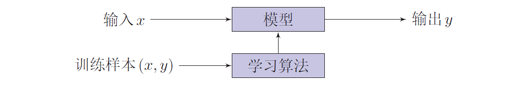
\includegraphics{pics/31.png}
 \caption{机器学习系统示意图}
 \label{fig:3.1}
\end{figure}
这里,$\hat{y}$是模型输出,$\theta$为决策函数的参数,$\phi(x)$ 表示样本$x$对应的特征表示。因为$x$不一定都是数值型的输入,因此需要通过$\phi(x)$ 将$x$转换为数值型的输入。如果我们假设$x$ 是已经处理好的标量或向量,公式\ref{3.1}也可以直接写为:
\begin{equation}\label{3.2}
  \hat{y}=f(x,\theta)
\end{equation}

此外,我们还要建立一些准则来衡量决策函数的好坏。在很多机器学习算法中,一般是定义一个损失函数$L(y, f(x, \theta))$,然后在所有的训练样本上来评价决策函数的风险:
\begin{equation}\label{3.3}
  R(\theta)=\frac{1}{N}\sum_{i=1}^{N}L(y^{(i)}, f(x^{(i)}, \theta))
\end{equation}

这里,风险函数$R(\theta)$是在已知的训练样本(经验数据)上计算得来的,因此被称之为\textbf{经验风险}。用对参数求经验风险来逐渐逼近理想的期望风险的最小值,就是我们常说的\textbf{经验风险最小化原则}(Empirical Risk Minimization)。这样,我们的目标就是变成了找到一个参数$\theta^{*}$使得经验风险最小。
\begin{equation}\label{3.4}
  \theta^{*}=\argmin_{\theta}R(\theta)\footnote{Given a function, $f\colon X \rightarrow Y$, the argmax over some subset, $S$, of $X$ is defined by $\underset{x\in S\subseteq X}{\operatorname{arg\,max}}\, f(x) := \{x \mid x\in S \wedge \forall y \in S : f(y) \le f(x)\}$. Obviously, $\underset{x}{\operatorname{arg\,max}}\, f(x) := \{x \mid \forall y : f(y) \le f(x)\}$.}
\end{equation}

因为用来训练的样本往往是真实数据的一个很小的子集或者包含一定的噪声数据,不能很好地反映全部数据的真实分布。经验风险最小化原则很容易导致模型在训练集上错误率很低,但是在未知数据上错误率很高。这就是所谓的\textbf{过拟合}(Overfit)。过拟合问题往往是由于训练数据少和噪声等原因造成的。过拟合的标准定义为:给定一个假设空间$H$,一个假设$h$ 属于$H$,如果存在其他的假设$\bar{h}$属于$H$, 使得在训练样例上$h$的损失比$\bar{h}$ 小,但在整个实例分布上$\bar{h}$比$h$的损失小,那么就说假设$h$ 过度拟合训练数据\cite{mitchell1998introduction}。

和过拟合相对应的一个概念是泛化错误,也称欠拟合。泛化错误是衡量一个机器学习模型是否可以很好地泛化到未知数据。泛化错误一般表现为一个模型在训练集和测试集上错误率的差距。

为了解决过拟合问题,一般在经验风险最小化的原则上上加参数的\textbf{正则化}(Regularization),也叫\textbf{结构风险最小化原则}(Structure Risk Minimization)。
\begin{gather}\label{3.5}
  \theta^{*}=\argmin_{\theta}R(\theta)+\lambda {\| \theta \|}_2^2\\
  =\argmin_{\theta}\frac{1}{N}\sum_{i=1}^{N}L(y^{(i)},f(x^{(i)}, \theta)) +\lambda {\| \theta \|}_2^2
\end{gather}
这里,${\| \theta \|}_2^2$是$L_2$范数的\textbf{正则化项},用来减少参数空间,避免过拟合。用$\lambda$来控制正则化的强度。
%\marginpar{margin text}
正则化项也可以使用其它函数,比如$L_1$范数。$L_1$ 范数的引入通常会使得参数有一定稀疏性,因此在很多算法中也经常使用。在Bayes 估计的角度来讲,正则化是假设了参数的先验分布,不完全依赖训练数据。
\subsection{补充问题:正则化}
在机器学习算法中,我们常常将原始数据集分为三部分:training data、validation data,testing data。这个validation data是什么?它其实就是用来避免过拟合的,在训练过程中,我们通常用它来确定一些超参数(比如根据validation data上的accuracy来确定early stopping的epoch大小、根据validation data确定learning rate等等)。那为啥不直接在testing data上做这些呢?因为如果在testing data做这些,那么随着训练的进行,我们的网络实际上就是在一点一点地overfitting我们的testing data,导致最后得到的testing accuracy没有任何参考意义。因此,training data的作用是计算梯度更新权重,validation data如上所述,testing data 则给出一个accuracy 以判断网络的好坏。

\begin{figure}[t]
 \centering
 \includegraphics{pics/Regu1.jpg}
 \caption{Overfit}
 \label{fig:Regu1}
\end{figure}

避免过拟合的方法有很多:early stopping、数据集扩增(Data augmentation)、正则化(Regularization)包括L1、L2(L2 regularization也叫weight decay),dropout。

\begin{itemize}
  \item \textbf{$L_0/L_1$ Regularization(Weight Decay)}:\\
  根据式\ref{3.5}可知,其中第一项$L(y^{(i)},f(x^{(i)}, \theta))$ 衡量我们的模型(分类或者回归)对第i 个样本的预测值$f(x^{(i)}, \theta)$和真实的标签$y^{(i)}$之前的误差。因为我们的模型是要拟合我们的训练样本的嘛,所以我们要求这一项最小,也就是要求我们的模型尽量的拟合我们的训练数据。但正如上面说言,我们不仅要保证训练误差最小,我们更希望我们的模型测试误差小,所以我们需要加上第二项,也就是对参数$\theta$的规则化函数$\Omega(\theta)$去约束我们的模型尽量的简单。\\
  其实大部分无非就是变换这两项而已。对于第一项Loss函数,如果是Square loss,那就是最小二乘了;如果是Hinge Loss,那就是SVM;如果是exp-Loss,那就是Boosting;如果是log-Loss,那就是Logistic Regression…… 不同的loss 函数,具有不同的拟合特性,这个也得就具体问题具体分析的。但这里,我们先不究loss函数的问题,我们把目光转向“规则项$\Omega(\theta)$”。\\
  规则化函数$\Omega(\theta)$也有很多种选择,一般是模型复杂度的单调递增函数,模型越复杂,规则化值就越大。比如,规则化项可以是模型参数向量的范数。然而,不同的选择对参数w的约束不同,取得的效果也不同,但在论文中常见的都聚集在:零范数、一范数、二范数、迹范数、Frobenius 范数和核范数等等。\\
  $L_0$范数是指向量中非0的元素的个数。如果我们用$L_0$范数来规则化一个参数矩阵$\boldsymbol{W}$的话,就是希望$\boldsymbol{W}$的大部分元素都是0。换句话说,让参数$\boldsymbol{W}$是稀疏\footnote{“压缩感知”和“稀疏编码”的“稀疏”就是这样来实现的。}但稀疏大多都通过$L_1$范数($||W||_1$)来实现的,因为二者在数学上有相当的关联。\\
  $L_1$范数是指向量中各个元素绝对值之和,也有个美称叫“稀疏规则算子”(Lasso regularization),它是$L_0$ 范数的最优凸近似。实际上,任何的规则化算子,如果他在$\boldsymbol{W}_i=0$的地方不可微,并且可以分解为一个“求和”的形式,那么这个规则化算子就可以实现稀疏。这说是这么说,$\boldsymbol{W}$的$L_1$范数是绝对值,$|\boldsymbol{W}|$在$\boldsymbol{W}=0$处是不可微,但这还是不够直观。因为$L_0$范数很难优化求解(NP难问题),二是$L_1$范数是$L_0$范数的最优凸近似,而且它比$L_0$范数要容易优化求解。\\
  \begin{equation*}
    \min||\boldsymbol{x}||_0~~s.t. \boldsymbol{A}\boldsymbol{x}=\boldsymbol{b}\overset{\text{概率为1 的}}{\underset{}{\iff}}\min||\boldsymbol{x}||_1~~s.t. \boldsymbol{A}\boldsymbol{x}=\boldsymbol{b}
  \end{equation*}
  参数稀疏的好处主要有以下两点:
  \begin{enumerate}
    \item 特征选择(Feature Selection)
    \item 可解释性(Interpretability)
  \end{enumerate}
  \item \textbf{$L_2$ Regularization(Weight Decay)}:\\
  除了$L_1$范数,还有一种更受青眯的规则化范数是$L_2$范数: $||\boldsymbol{W}||_2$。它也不逊于$L_1$范数,在回归里面,有人把有它的回归叫“岭回归”(Ridge Regression),有人也叫它“权值衰减weight decay”。这用的很多吧,因为它的强大功效是改善机器学习里面一个非常重要的问题:过拟合。\\
  $L_2$范数是指向量各元素的平方和然后求平方根。我们让L2范数的规则项$||\boldsymbol{W}||_2$ 最小,可以使得W 的每个元素都很小,都接近于0,但与$L_1$ 范数不同,它不会让它等于0,而是接近于0,这里是有很大的区别。而越小的参数说明模型越简单,越简单的模型则越不容易产生过拟合现象。限制了参数很小,实际上就限制了多项式某些分量的影响很小,这样就相当于减少参数个数。\\
  除了防止过拟合和提升模型的泛化能力的问题外,$L_2$范数还能够在计算优化的角度上对处理 condition number\footnote{
  首先假定只存在$\boldsymbol{b}$的扰动$\delta\boldsymbol{b}$,$\boldsymbol{A}$稳定,考察$\boldsymbol{A}\boldsymbol{x}=\boldsymbol{b}$ 的解析解向量$\boldsymbol{x}+\delta\boldsymbol{x}$,即:
  \begin{equation*}
    \boldsymbol{A}(\boldsymbol{x}+\delta\boldsymbol{x})=\boldsymbol{b}+\delta\boldsymbol{b}
  \end{equation*}
  求解得:
  \begin{equation*}
    \delta\boldsymbol{x}=\boldsymbol{A}^{-1}\delta\boldsymbol{b}
  \end{equation*}
  由向量范数性质:
  \begin{equation*}
    ||\delta\boldsymbol{x}||_2\leq||\boldsymbol{A}^{-1}||_2\cdot||\delta\boldsymbol{b}||_2
  \end{equation*}
  同理显然:
  \begin{equation*}
    ||\boldsymbol{b}||_2\leq||\boldsymbol{A}||_2\cdot||\boldsymbol{x}||_2
  \end{equation*}
  于是:
  \begin{equation*}
    \frac{||\delta\boldsymbol{x}||_2}{||\boldsymbol{x}||_2}\leq||\boldsymbol{A}||_2\cdot||\boldsymbol{A}^{-1}||_2\frac{||\delta\boldsymbol{b}||_2}{||\boldsymbol{b}||_2}
  \end{equation*}

  然后考察$\delta\boldsymbol{A}$的影响:
  \begin{equation*}
    (\boldsymbol{A}+\delta\boldsymbol{A})(\boldsymbol{x}+\delta\boldsymbol{x})=\boldsymbol{b}
  \end{equation*}
  同理显然:
  \begin{equation*}
    \frac{||\delta\boldsymbol{x}||_2}{||\boldsymbol{x}||_2+||\delta\boldsymbol{x}||_2}\leq||\boldsymbol{A}||_2\cdot||\boldsymbol{A}^{-1}||_2\frac{||\delta\boldsymbol{A}||_2}{||\boldsymbol{A}||_2}
  \end{equation*}

  于是可知解向量的相对误差应正比于$||\boldsymbol{A}||_2\cdot||\boldsymbol{A}^{-1}||_2\equiv\text{cond}(\boldsymbol{A})\equiv\kappa(\boldsymbol{A})$,称condition number.

  对于超定方程($\boldsymbol{A}\in\mathbb{C}^{m\times n}(m>n)$),必有最小二乘解$\boldsymbol{x}=(\boldsymbol{A}^H\boldsymbol{A})^{-1}\boldsymbol{A}^H\boldsymbol{b}$。 容易证明(你信么?)$\text{cond}(\boldsymbol{A}^H\boldsymbol{A})=\text{cond}^2(\boldsymbol{A})$。 条件数是平方关系增大的,同时稳定性反比于条件数。
  }不好的情况下矩阵求逆很困难的问题。condition number是一个矩阵(或者它所描述的线性系统)的稳定性或者敏感度的度量,如果一个矩阵的condition number在1 附近,那么它就是well-conditioned 的,如果远大于1,那么它就是ill-conditioned 的,如果一个系统是ill-conditioned的,它的输出结果就不具有相当的置信度。\\
  从优化或者数值计算的角度来说,$L_2$范数有助于处理 condition number不好的情况下矩阵求逆很困难的问题。因为目标函数如果是二次的,对于线性回归来说,那实际上是有解析解的,求导并令导数等于零即可得到最优解为:
  \begin{equation*}
    \boldsymbol{W}=(\boldsymbol{X}^H\boldsymbol{X})^{-1}\boldsymbol{X}^H\boldsymbol{y}
  \end{equation*}
  然而,如果当我们的样本X的数目比每个样本的维度还要小的时候,矩阵$\boldsymbol{X}^H\boldsymbol{X}$将会不是满秩的,所以$\boldsymbol{W}$无法直接计算。或者更确切地说,将会有无穷多个解(因为我们方程组的个数小于未知数的个数)。也就是说,我们的数据不足以确定一个解,如果我们从所有可行解里随机选一个的话,很可能并不是真正好的解,即是出现过拟合。\\
  但如果加上L2规则项,就变成了下面这种情况,就可以直接求逆了:
  \begin{equation*}
    \boldsymbol{W}=(\boldsymbol{X}^H\boldsymbol{X}+\lambda\boldsymbol{I})^{-1}\boldsymbol{X}^H\boldsymbol{y}
  \end{equation*}
  这个规则项的引入则可以改善condition number.

  如果使用迭代优化的算法,condition number 太大仍然会导致问题:它会拖慢迭代的收敛速度,而规则项从优化的角度来看,实际上是将目标函数变成$\lambda$-strongly convex\footnote{
  A differentiable function $f$ is called \textbf{$\lambda$-strongly convex} with parameter $\lambda > 0$ if the following inequality holds for all points x, y in its domain:
  \begin{equation*}
    ( \nabla f(x) - \nabla f(y) )^T (x-y) \ge \lambda \|x-y\|_2^2
  \end{equation*}
  or, more generally,
  \begin{equation*}
    \langle \nabla f(x) - \nabla f(y),  (x-y) \rangle \ge \lambda \|x-y\|^2
  \end{equation*}
  where $\|\cdot\|$ is any norm.
  }($\lambda$强凸)的,也即可以在迭代中避免大平原的情况.
  \item \textbf{Dropout}:\\
  L1、L2正则化是通过修改代价函数来实现的,而Dropout则是通过修改神经网络本身来实现的,它是在训练网络时用的一种技巧。它的流程如图\ref{fig:Regu2}:\\
  假设我们要训练上图这个网络,在训练开始时,我们随机地“删除”一半的隐层单元,视它们为不存在;保持输入输出层不变,按照BP算法更新上图神经网络中的权值(虚线连接的单元不更新,因为它们被“临时删除”了)。\\
  以上就是一次迭代的过程,在第二次迭代中,也用同样的方法,只不过这次删除的那一半隐层单元,跟上一次删除掉的肯定是不一样的,因为我们每一次迭代都是“随机”地去删掉一半。第三次、第四次……都是这样,直至训练结束。\\
  以上就是Dropout,它为什么有助于防止过拟合呢?可以简单地这样解释,运用了dropout的训练过程,相当于训练了很多个只有半数隐层单元的神经网络(后面简称为“半数网络”),每一个这样的半数网络,都可以给出一个分类结果,这些结果有的是正确的,有的是错误的。随着训练的进行,大部分半数网络都可以给出正确的分类结果,那么少数的错误分类结果就不会对最终结果造成大的影响。
  %更加深入地理解,可以看看Hinton和Alex 两牛2012的论文《ImageNet Classification with Deep Convolutional Neural Networks》

  \begin{figure}[t]
 \centering
 \includegraphics{pics/Regu2.jpg}
 \caption{Dropout}
 \label{fig:Regu2}
 \end{figure}
  \item \textbf{数据集扩增(Data Augmentation)}:\\
  在深度学习方法中,更多的训练数据,意味着可以用更深的网络,训练出更好的模型。\\
  如果能够收集更多可以用的数据,当然好。但是很多时候,收集更多的数据意味着需要耗费更多的人力物力,效率低下。\\
  所以,可以在原始数据上做些改动,得到更多的数据,以图片数据集举例,可以做各种变换,如:
  \begin{enumerate}
    \item 将原始图片旋转一个小角度
    \item 添加随机噪声
    \item 一些有弹性的畸变(elastic distortions),论文\cite{simard2003best}对MNIST做了各种变种扩增。
    \item 截取(crop)原始图片的一部分。比如DeepID中,从一副人脸图中,截取出了100个小patch 作为训练数据,极大地增加了数据集\cite{sun2014deep}。
  \end{enumerate}

  更多数据意味着什么?用50000个MNIST的样本训练SVM得出的accuracy 为94.48\%,用5000个MNIST 的样本训练NN得出accuracy为93.24\%,所以更多的数据可以使算法表现得更好。在机器学习中,算法本身并不能决出胜负,不能武断地说这些算法谁优谁劣,因为数据对算法性能的影响很大。

  \item \textbf{Early Stopping}:\\
  所谓early stopping,即在每一个epoch结束时(一个epoch即对所有训练数据的一轮遍历)计算 validation data的accuracy,当accuracy不再提高时,就停止训练。这是很自然的做法,因为accuracy不再提高了,训练下去也没用。另外,这样做还能防止overfitting。

  那么,怎么样才算是validation accuracy 不再提高呢?并不是说validation accuracy一降下来,它就是“不再提高”,因为可能经过这个epoch后,accuracy降低了,但是随后的epoch又让accuracy升上去了,所以不能根据一两次的连续降低就判断“不再提高”。正确的做法是,在训练的过程中,记录最佳的validation accuracy,当连续10 次epoch (或者更多次)没达到最佳accuracy时,你可以认为“不再提高”,此时使用early stopping。这个策略就叫“ no-improvement-in-n”,n即epoch的次数,可以根据实际情况取10、20、30….
\end{itemize}
\subsection{损失函数}
一个实例$(x, y)$,真实目标是$y$,机器学习模型的预测为$f(x, \theta)$。 如果预测错误时($f(x, \theta) \not= y)$,我们需要定义一个度量函数来定量地计算错误的程度。常见的损失函数有如下几类:

\textbf{0-1 损失函数}(0-1 loss function)
\begin{equation}\label{3.7}
  L(y^{(i)}, f(x^{(i)}, \theta))=I(y=f(x,\theta))
\end{equation}
这里$I$是特征函数。

\textbf{平方损失函数}(quadratic loss function)
\begin{equation}\label{3.8}
  L(y,\hat{y})=(y-f(x,\theta))^2
\end{equation}

\textbf{交叉熵损失函数}\\
对于分类问题,预测目标$y$的离散类别,模型输出$f(x,\theta)$为每个类别的条件概率。

假设$y\in \{1,\dots\,C\}$,模型预测的第$i$ 类的条件概率$P(y=i|x)=f_i(x,\theta)$,则$f(x,\theta)$满足:
\begin{equation}\label{3.9}
  f_i(x,\theta)\in [0,1],   \sum_{i=1}^C f_i(x,\theta)=1
\end{equation}

$f_y(x,\theta)$可以看作真实类别$y$的似然函数。参数可以直接用最大似然估计来优化。考虑到计算问题,我们经常使用最小化负对数似然,也就是负对数似然损失函数(Negative Log Likelihood function)。
\begin{equation}\label{3.10}
  L(y,f(x,\theta))=-\log f_y(x,\theta)
\end{equation}

如果我们用one-hot向量\footnote{在数字电路中,one-hot 是一种状态编码,指对任意给定的状态,状态寄存器中只有l 位为1,其余位都为0。}$\boldsymbol{y}$来表示目标类别$c$,其中只有$y_c = 1$,其余的向量元素都为0。

负对数似然函数也可以写为:
\begin{equation}\label{3.11}
  L(y,f(x,\theta))=-\sum_{i=1}^C y_i \log f_y(x,\theta)
\end{equation}

$y_i$ 也也可以看成是真实类别的分布,这样公式\ref{3.11}恰好是交叉熵的形式。因此,负对数似然损失函数也常叫做交叉熵损失函数(Cross Entropy Loss function)是负对数似然函数的一种改进。
\\

\textbf{Hinge损失函数}(Hinge Loss Function)
对于两类分类问题,假设$y$和$f(x, \theta)$ 的取值为$\{-1,+1\}$。Hinge 损失函数的定义如下:
\begin{equation}\label{3.12}
  L(y,f(x,\theta))=\max(0,1-yf(x,\theta))=|1-yf(x,\theta)|_+
\end{equation}

\subsection{补充问题:机器学习与信息论的关系}
信息论与机器学习同为涉及计算机科学和应用数学等学科的分支领域,这两门交叉学科在起源和应用上有很多相似之处。信息论的理论体系相对成熟一些。机器学习这些年比较受欢迎,理论和应用的扩充发展速度远远更快且看不到饱和的趋势。两个方向互有交叉,但主要还是机器学习中借用信息论的方法以此拓展理论研究和应用场景,比较典型的就是借鉴信息理论创造和改进学习算法(主要是分类问题),甚至衍生出了一个新方向,信息理论学习,详细介绍和研究近况可以参考\cite{principe2000information}
\begin{figure}[b]
 \centering
 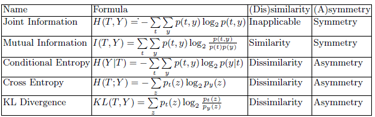
\includegraphics{pics/32.png}
 \caption{Some information formulas and their properties as learning measures}
 \label{fig:3.2}
\end{figure}

以上结论,以下具体说明。

机器学习可以根据数学原理分为两种,一种基于经验公式(错误率、边界、代价、风险、实用性、分类边缘),还有一种则是基于信息理论。

信息论中的一些度量也可以作为学习算法的度量。Watanabe也提出过“\textbf{学习就是一个熵减的过程}”,学习的过程也就是使信息的不确定度下降的过程。Bayesian理论也扎根于信息和优化的概念中。比起传统的经验公式为基础的机器学习,以信息理论为基础的机器学习也拥有无可比拟的优势。当少数类的样本数量接近0时,Bayesian分类器对少数类的分类趋向于完全的错误。而以互信息为学习准则的分类器则能够保护少数类,并根据各类样本数量比例自动平衡错误型和拒绝型。


有目标随机变量$T$和预测结果随机变量$Y$,那么有图\ref{fig:3.2} 的关系。


这些度量中,互信息可以用来衡量相似性,而条件熵、交叉熵和相对熵可以用来度量相异性。

如果一个变量$T$在统计意义上提供真实值(也就是说$p(t)=(p_1,\dots,p_m)$ 其中总体率$p_i(i=1,\dots,m)$已知),那么它的熵$H(T)$ 就是学习的基线,也就是说出现这种情况$I(T,Y)=H(T;Y)=H(Y;T)=H(Y)=H(T)$ 或这种情况$KL(T,Y)=KL(Y,T)=H(Y|T)=H(T|Y)=0$ 时我们就可以说,我们就说这种方法达到了基线H(T).


对于这些量的关系如图\ref{fig:3.3}所示:

\begin{figure}[t]
 \centering
 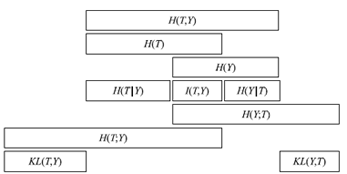
\includegraphics{pics/33.png}
 \caption{The relationship among some measures}
 \label{fig:3.3}
\end{figure}
\begin{figure}[t]
 \centering
 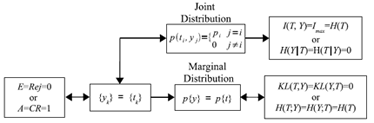
\includegraphics{pics/34.png}
 \caption{The relationship among $E,Rej,A,CR$}
 \label{fig:3.4}
\end{figure}

我们记$E,Rej,A,CR$分别表示错误率,拒绝率,正确率和正确识别率。那么有$CR+E+Rej=1$和$A=\frac{CR}{CR+E}$,这时有如图\ref{fig:3.4}所示关系\cite{mackay2003information}

这里的$\{y_k\}=\{t_k\}$表示每个对应标签样本之间都相等。对于有限的数据集来说,这种形式用来表示分布和度量,用$\leftrightarrow$ 表示对于等价关系的双向连接,用$\rightarrow$表示单向连接。
\begin{itemize}
  \item 准确分类的必要条件是所有信息度量都达到了基线
  \item 当所有信息度量都达到了基线,也不能充分说明这是准确分类
  \item 单向连接的不同位置解释了充分条件为什么存在以及充分条件是什么
\end{itemize}

当然当遇到其他问题的时候我们还可以扩展到其他信息度量,比如聚类、特征选择/提取等。当我们从相似度(或者也能转变成相似度的相异度)着手来考虑机器学习/模式识别的过程的时候,有一个重要的定理用以描述它们的关系:一般来说,在经验定义的相似度量和信息度量之间,不存在一对一的对应关系(这个结论由错误和熵的学习边界的研究给出)。

所以,由信息度量的优化并不能保证获得经验方法完成的优化效果。

但是,也有不少研究者猜想\cite{hu2015information},在机器学习中,所有学习目标的computational representation 都是可以用熵函数的优化来描述或者解释的。这个猜想给了我们很好的一个研究着力的方向。

上面的概述比较抽象了,那么最后看一个简单的实例,如图\ref{fig:3.5}所示:

以互信息作为学习准则。例如以应用信息增益(归一化的互信息)构造最简结构决策树就是其中一种应用。这种基于信息理论为学习准则的原理就是将无序(标签、特征)数据转变为有序数据,以信息熵差值作为测量尺度来评价转换效果。

\begin{figure}[t]
 \centering
 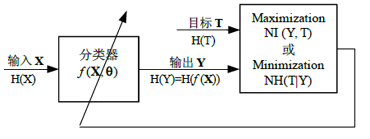
\includegraphics{pics/35.png}
 \caption{Example}
 \label{fig:3.5}
\end{figure}

现在的研究有关于怎样设计目标函数,怎样处理其中互信息、经验熵的计算,互信息与分类器传统性能指标的关系?

还有具体实例也暂时没想到怎么表述,另外除了常用的几个,应用较多的如Renyi entropy 也等待补充……


\subsection{机器学习算法的类型}
根据训练数据提供的信息以及反馈方式的不同,机器学习算法一般可以分为以下几类:

\textbf{有监督学习}(Supervised Learning) 有监督学习是利用一组已知输入$x$和输出$y$的数据来学习模型的参数,使得模型预测的输出标记和真实标记尽可能的一致。有监督学习根据输出类型又可以分为\textbf{回归}和\textbf{分类}两类。

\textbf{回归}(Regression) 如果输出$y$是连续值(实数或连续整数),$f(x)$的输出也是连续值。这种类型的问题就是回归问题。对于所有已知或未知的$(x, y)$,使得$f(x, \theta)$ 和$y$尽可能地一致。损失函数通常定义为平方误差。
\begin{equation}\label{3.13}
  L(y,f(x,\theta))=\|y-f(x,\theta)\|^2
\end{equation}

\textbf{分类}(Classification) 如果输出$y$是离散的类别标记(符号),就是分类问题。损失函数有很多种定义方式。一种常用的方式就是0-1 损失函数。
\begin{equation}\label{3.14}
  L(\hat(y),y)=I(f(x,\theta)=y)
\end{equation}
这里$f(x, \theta)$的输出也是离散值,$I(\cdot)$ 是特征函数.另一种常用的方式是让$f_i(x, \theta)$ 去估计给定$x$的情况下第$i$ 个类别的条件概率$P(y = i|x)$。损失函数定义为负对数似然函数。

在分类问题中,通过学习得到的决策函数$f(x, \theta)$也叫分类器。

\textbf{无监督学习}(Unsupervised Learning) 无监督学习是用来学习的数据不包含输出目标,需要学习算法自动学习到一些有价值的信息。一个典型的无监督学习问题就是\textbf{聚类}(Clustering)。

\textbf{增强学习}(Reinforcement Learning) 增强学习也叫强化学习,强调如何基于环境做出一系列的动作,以取得最大化的累积收益。每做出一个动作,并不一定立刻得到收益。增强学习和有监督学习的不同在于增强学习不需要显式地以输入/输出对的方式给出训练样本,是一种在线的学习机制。


有监督的学习方法需要每个数据记录都有类标号,而无监督的学习方法则不考虑任何指导性信息。一般而言,一个监督学习模型需要大量的有标记数据集,而这些数据集是需要人工标注的。因此,也出现了很多弱监督学习和半监督学习的方法,希望从大规模的未标记数据中充分挖掘有用的信息,降低对标记数据数量的要求。

\subsection{机器学习中的一些基本概念}
上述的关于机器学习的介绍中,提及了一些基本概念,比如“数据”,“样本”,“特征”,“数据集”等。我们首先来解释下这些概念。\\

\textbf{数据}
在计算机科学中,数据是指所有能计算机程序处理的对象的总称,可以是数字、字母和符号等。在不同的任务中,表现形式不一样,比如图像、声音、文字、传感器数据等。\\

\textbf{特征}
机器学习中很多算法的输入要求是数学上可计算的。而在现实世界中,原始数据通常是并不都以连续变量或离散变量的形式存在的。我们首先需要将抽取出一些可以表征这些数据的数值型特征。这些数值型特征一般可以表示为向量形式,也称为特征向量。\\

\textbf{特征学习}
数据的原始表示转换为。原始数据的特征有很多,但是并不是所有的特征都是有用的。并且,很多特征通常是冗余并且易变的。我们需要抽取有效的、稳定的特征。传统的特征提取是通过人工方式进行的,这需要大量的人工和专家知识。即使这样,人工总结的特征在很多任务上也不能满足需要。因此,如何自动地学习有效的特征也成为机器学习中一个重要的研究内容,也就是\textbf{特征学习},也叫\textbf{表示学习}。特征学习分成两种,一种是\textbf{特征选择},是在很多特征集合选取有效的子集;另一种是\textbf{特征提取},是构造一个新的特征空间,并将原始特征投影在新的空间中。\\

\textbf{样本}
样本是按照一定的抽样规则从全部数据中取出的一部分数据,是实际观测得到的数据。在有监督学习中,需要提供一组有输出目标的样本用来学习模型以及检验模型的好坏。\\

\textbf{训练集和测试集}
一组样本集合就称为\textbf{数据集}。在很多领域,数据集也经常称为\textbf{语料库}。为了检验机器学习算法的好坏,一般将数据集分为两部分:训练集和测试集。训练集用来进行模型学习,测试集用来进行模型验证。通过学习算法,在训练集得到一个模型,这个模型可以对测试集上样本$x$预测一个类别标签$\hat{y}$。假设测试集为$T$, 模型的正确率为:
\begin{equation}\label{3.15}
  Acc=\frac{1}{|T|}\sum_{(x_i,y_i)\in T}|\hat{y_i}=y_i|
\end{equation}
其中$|T|$为测试集的大小。后面中会介绍更多的评价方法。\\

\textbf{正例和负例}
对于两类分类问题,类别可以表示为$\{+1, -1\}$,或者直接用正负号表示。因此,常用正例和负例来分别表示属于不同类别的样本。\\

\textbf{判别函数}
经过特征抽取后,一个样本可以表示为$k$维特征空间中的一个点。为了对这个特征空间中的点进行区分,就需要寻找一些超平面来将这个特征空间分为一些互不重叠的子区域,使得不同类别的点分布在不同的子区域中,这些超平面就成为判别界面。
为了定义这些用来进行空间分割的超平面,就需要引入判别函数的概念。假设变量$\boldsymbol{z} \in \mathbb{R}^m$为特征空间中的点,这个超平面由所有满足函数$f(\boldsymbol{z}) = 0$的点组成。这里的$f(\boldsymbol{z})$ 就称为\textbf{判别函数}。
有了判别函数,分类就变得很简单,就是看一个样本在特征空间中位于哪个区域,从而确定这个样本的类别。
判别函数的形式多种多样,在自然语言处理中,最为常用的判别函数为线性函数。

\subsection{参数学习方法}
\textbf{学习算法}就是如何从训练集的样本中,自动学习决策函数的参数。不同机器学习算法的区别在于决策函数和学习算法的差异。相同的决策函数可以有不同的学习算法。比如线性分类器,其参数的学习算法可以是感知器、支持向量机以及梯度下降法等。通过一个学习算法进行自动学习参数的过程也叫作\textbf{训练过程}。

这里我们介绍一种常用的参数学习算法:\textbf{梯度下降法}(Gradient Descent Method)。

梯度下降法也叫最速下降法(Steepest Descend Method)。如果一个实值函数$f(\boldsymbol{x})$在点$\boldsymbol{a}$ 处可微且有定义,那么函数$f(\boldsymbol{x})$ 在$\boldsymbol{a}$点沿着梯度相反的方向$-\nabla f(\boldsymbol{a})$下降最快。梯度下降法经常用来求解无约束优化的极值问题。梯度下降法的迭代公式为:
\begin{equation}\label{3.16}
  \boldsymbol{a}_{t+1}=\boldsymbol{a}_{t}-\lambda\nabla f(\boldsymbol{a}_{t})
\end{equation}
其中$\lambda>0$是梯度方向上的搜索步长。

对于$\lambda$为一个足够小的数值是,那么$f(\boldsymbol{a}_{t+1})\leq f(\boldsymbol{a}_{t})$.因此,我们可以从一个初始值$\boldsymbol{x_0}$ 开始,并通过迭代公式得到$\boldsymbol{x_0}, \boldsymbol{x_1}, \boldsymbol{x_2},\dots,\boldsymbol{x_n}$,并满足:
\begin{equation*}
  f(\boldsymbol{x}_0)\geq f(\boldsymbol{x}_1)\geq f(\boldsymbol{x}_2)\geq \dots\geq f(\boldsymbol{x}_n)
\end{equation*}
最终$\boldsymbol{x_n}$收敛到期望的极值。

搜索步长的取值必须合适,如果过大就不会收敛,如果过小则收敛速度太慢。一般步长可以由线性搜索算法来确定。

在机器学习问题中,我们需要学习到参数$\theta$,使得风险函数最小化。
\begin{gather}\label{3.17}
  \theta^{*}=\arg\min_{\theta}\mathcal{R}(\theta_t)\\
  =\arg\min_{\theta}\frac{1}{N}\sum_{i=1}^{N}\mathcal{L}(y^{(i)},f(x^{(i)},\theta))
\end{gather}

如果用梯度下降法进行参数学习,
\begin{gather}\label{3.19}
  \boldsymbol{a}_{t+1}=\boldsymbol{a}_{t}-\lambda\frac{\partial \mathcal{R}(\theta)}{\partial \theta_t}\\
  =\boldsymbol{a}_{t}-\lambda\sum_{i=1}^N\frac{\partial \mathcal{R}(\theta_t;x^{(i)},y^{(i)})}{\partial \theta}
\end{gather}
$\lambda$在机器学习中也叫作\textbf{学习率}(Learning Rate)

这里,梯度下降是求得所有样本上的风险函数最小值,叫做\textbf{批量梯度下降法}。若样本个数$N$很大,输入$x$的维数也很大时,那么批量梯度下降法每次迭代要处理所有的样本,效率会较低。为此,有一种改进的方法即\textbf{随机梯度下降法}。

随机梯度下降法(Stochastic Gradient Descent,SGD)也叫\textbf{增量梯度下降},每个样本都进行更新:
\begin{equation}\label{3.20}
  \boldsymbol{a}_{t+1}=\boldsymbol{a}_{t}-\lambda\frac{\partial \mathcal{R}(\theta_t;x^{(t)},y^{(t)})}{\partial \theta}
\end{equation}
$x^{(t)},y^{(t)}$是第$t$次迭代选取的样本。

批量梯度下降和随机梯度下降之间的区别在于每次迭代的风险是对所有样本汇总的风险还是单个样本的风险。随机梯度下降因为实现简单,收敛速度也非常快,因此使用非常广泛。

还有一种折中的方法就是\textbf{mini-batch随机梯度下降},每次迭代时,只采用一小部分的训练样本,兼顾了批量梯度下降和随机梯度下降的优点。\\

\textbf{Early-Stop}
在梯度下降训练的过程中,由于过拟合的原因,在训练样本上收敛的参数,并不一定在测试集上最优。因此,我们使用一个\textbf{验证集}(Validation Dataset)(也叫\textbf{开发集}(Development Dataset))来测试每一次迭代的参数在验证集上是否最优。如果在验证集上的错误率不再下降,就停止迭代。这种策略叫Early-Stop。如果没有验证集,可以在训练集上进行\textbf{交叉验证}。\\

\textbf{学习率设置}
在梯度下降中,学习率的取值非常关键,如果过大就不会收敛,如果过小则收敛速度太慢。一般步长可以由线性搜索算法来确定。在机器学习中,经常使用自适应调整学习率的方法。

\textbf{动量法}(Momentum Method)\cite{rumelhart1988learning} 对当前迭代的更新中加入上一次迭代的更新。我们记$\nabla \theta_t = \theta_t-\theta_{t-1}$。 在第$t$迭代时,
\begin{equation}\label{3.21}
  \theta_t = \theta_{t-1} +(\rho\nabla\theta_{t}-\lambda g_t)
\end{equation}
其中,$\rho$为动量因子,通常设为0.9。这样,在迭代初期,使用前一次的梯度进行加速。在迭代后期的收敛值附近,因为两次更新方向基本相反,增加稳定性。

\textbf{AdaGrad}(Adaptive Gradient)算法\cite{duchi2011adaptive} 是借鉴$L_2$ 正则化的思想。在第$t$迭代时,
\begin{equation}\label{3.22}
  \theta_t = \theta_{t-1}-\frac{\rho}{\sqrt{\sum_{\tau=1}^t g_{\tau}^2}}g_t
\end{equation}
其中,$\rho$是初始学习率,$g_{\tau}\in \mathbb{R}^{|\theta|}$ 是第$\tau$次迭代时的梯度。

随着迭代次数的增加,梯度逐渐缩小。

\textbf{AdaDelta} 算法\cite{zeiler2012adadelta} 用指数衰减的移动平均来累积历史的梯度信息。第$t$ 次迭代的梯度的期望$E(g^2)_t$ 为:
\begin{equation}\label{3.23}
  E(g^2)_t=\rho E(g^2)_{t-1}+(1-\rho g_t^2)
\end{equation}
其中$\rho$是衰减常数。

本次迭代更新为:
\begin{equation}\label{3.24}
  \nabla\theta_t=-\frac{\sqrt{E(\nabla\theta^2)_{t-1}+\epsilon}}{\sqrt{E(g^2)_{t}+\epsilon}}g_t
\end{equation}
其中,$E(\nabla\theta^2)_t$为前一次迭代时$\nabla\theta^2$的移动平均,$\epsilon$ 为常数。

最后更新参数:
\begin{equation}\label{3.25}
  \theta_t=\theta_{t-1}+\nabla\theta_t
\end{equation}

\section{线性回归}
如果输入$\boldsymbol{x}$是列向量,目标$y$ 是连续值(实数或连续整数),预测函数$f(\boldsymbol{x})$ 的输出也是连续值。这种机器学习问题是回归问题。

如果我们定义$f(\boldsymbol{x})$是线性函数,那么
\begin{equation}\label{3.26}
  f(\boldsymbol{x})=\boldsymbol{w}^T\boldsymbol{x}+b
\end{equation}
就是线性回归问题(Linear Regression)。

为了简单起见,我们将公式\ref{3.26}写为:
\begin{equation}\label{3.27}
  f(\boldsymbol{x})=\hat{\boldsymbol{w}}^T\hat{\boldsymbol{x}}
\end{equation}

\section{线性分类}
\subsection{二类分类}
\subsection{多类线性分类}
\section{评价方法}
\section{进一步的阅读和总结}
为更加深入地理解Dropout,可以翻阅论文:《ImageNet Classification with Deep Convolutional Neural Networks》

\chapterimage{chapter_head_4.jpg}
\chapter{感知器}
\section{二类感知器}
\subsection{感知器学习算法}
\subsection{线性感知器收敛性证明}
\section{多类感知器}
\subsection{多类感知器收敛性证明}
\section{投票感知器}
%---------------------------------------------
\chapterimage{chapter_head_5.jpg}
\section{进一步的阅读和总结}

\chapter{人工神经网络}
人工神经网络1943年,心理学家W.S.McCulloch 和数理逻辑学家W.Pitts建立了神经网络和数学模型,称为MP 模型。他们通过MP模型提出了神经元的形式化数学描述和网络结构方法,证明了单个神经元能执行逻辑功能,从而开创了人工神经网络研究的时代。1949年,心理学家提出了突触联系强度可变的设想。60年代,人工神经网络得到了进一步发展,更完善的神经网络模型被提出人工神经网络人工神经网络,其中包括感知器和自适应线性元件等。

前馈神经网络也经常称为\textbf{多层感知器}(Multilayer Perceptron,MLP)。但多层感知器的叫法并不是否合理,因为前馈神经网络其实是由多层的logistic回归模型(连续的非线性函数)组成,而不是有多层的感知器(不连续的非线性函数)组成\cite{bishop2006pattern}。人工神经网络(Artificial Neural Network,即ANN),是20世纪80 年代以来人工智能领域兴起的研究热点。它从信息处理角度对人脑神经元网络进行抽象,建立某种简单模型,按不同的连接方式组成不同的网络。在工程与学术界也常直接简称为神经网络或类神经网络。神经网络是一种运算模型,由大量的节点(或称神经元)之间相互联接构成。每个节点代表一种特定的输出函数,称为激励函数(activation function)。每两个节点间的连接都代表一个对于通过该连接信号的加权值,称之为权重,这相当于人工神经网络的记忆。网络的输出则依网络的连接方式,权重值和激励函数的不同而不同。而网络自身通常都是对自然界某种算法或者函数的逼近,也可能是对一种逻辑策略的表达。最近十多年来,人工神经网络的研究工作不断深入,已经取得了很大的进展,其在模式识别、智能机器人、自动控制、预测估计、生物、医学、经济等领域已成功地解决了许多现代计算机难以解决的实际问题,表现出了良好的智能特性。

人工神经网络模型主要考虑网络连接的拓扑结构、神经元的特征、学习规则等。目前,已有近40种神经网络模型,其中有反传网络、感知器、自组织映射、Hopfield 网络、波耳兹曼机、适应谐振理论等。根据连接的拓扑结构,神经网络模型可以分为:
\begin{itemize}
  \item 前向网络:
  网络中各个神经元接受前一级的输入,并输出到下一级,网络中没有反馈,可以用一个有向无环路图表示。这种网络实现信号从输入空间到输出空间的变换,它的信息处理能力来自于简单非线性函数的多次复合。网络结构简单,易于实现。反传网络是一种典型的前向网络。
  \item 反馈网络:
  网络内神经元间有反馈,可以用一个无向的完备图表示。这种神经网络的信息处理是状态的变换,可以用动力学系统理论处理。系统的稳定性与联想记忆功能有密切关系。Hopfield网络、波耳兹曼机均属于这种类型。
\end{itemize}
\section{神经元}
人工神经元(Neuron)是构成人工神经网络的基本单元。人工神经元和感知器非常类似,也是模拟生物神经元特性,接受一组输入信号并产出输出。生物神经元有一个阀值,当神经元所获得的输入信号的积累效果超过阀值时,它就处于兴奋状态;否则,应该处于抑制状态。

人工神经元使用一个非线性的激活函数,输出一个活性值。假定神经元接受$n$个输入$\boldsymbol{x} = (x_1,x_2,\cdots ,x_n)$,用状态$z$表示一个神经元所获得的输入信号$x$ 的加权和,输出为该神经元的活性值$a$。 具体定如下:
\begin{equation*}
  z=\boldsymbol{w}^T\boldsymbol{x}+b
\end{equation*}
\begin{equation*}
  a=f(z)
\end{equation*}
其中,$\boldsymbol{w}$是$n$维的权重向量,$b$是偏置。典型的激活函数$f$ 有sigmoid型函数、非线性斜面函数等。

人工神经元的结构如图\ref{fig:5.1}所示。如果我们设激活函数$f$为0或1的阶跃函数,人工神经元就是感知器。

\begin{figure}[t]
 \centering
 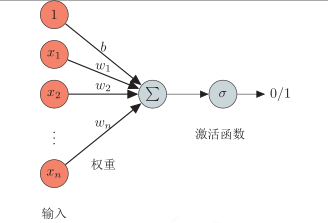
\includegraphics{pics/51.png}
 \caption{Neuron}
 \label{fig:5.1}
\end{figure}
\subsection{激活函数}
为了增强网络的表达能力,我们需要引入连续的非线性激活函数(Activation Function)。因为连续非线性激活函数可以可导的,所以可以用最优化的方法来求解。传统神经网络中最常用的激活函数分别是sigmoid 型函数。sigmoid型函数是指一类S 型曲线函数,常用的sigmoid型函数有logistic函数$\sigma(x)$和tanh函数。

在第二章的常用函数中已经叙述了他们的定义和一些简单性质。
\begin{equation*}
  \tanh(x)=\frac{\exp{(x)}-\exp{(-x)}}{\exp{(x)}+\exp{(-x)}}=2\sigma(2x)-1
\end{equation*}
tanh函数可以看作是放大并平移的logistic函数.

sigmoid型函数对中间区域的信号有增益,对两侧区的信号有抑制。这样的特点也和生物神经元类似,对一些输入有兴奋作用,另一些输入(两侧区)有抑制作用。和感知器的阶跃激活函数$(-1/1,0/1)$相比,sigmoid型函数更符合生物神经元的特性,同时也有更好的数学性质很好。
\begin{figure}[t]
 \centering
 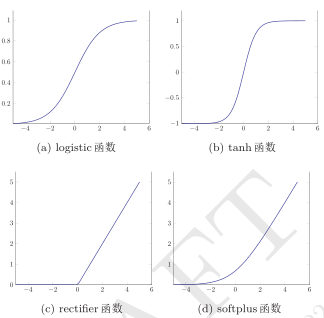
\includegraphics{pics/52.png}
 \caption{Activation Function}
 \label{fig:5.2}
\end{figure}
\subsection{激活函数的表达能力}
如果每层都是完全线性的激活函数,会导致神经网络退化成LR,一般不会选择这种激活函数,虽然其表达能力虽然同LR 一致,然而训练过程高度非线性,完全异于LR,用于非常初期的深层网络训练理论研究是有帮助的。

每层都是sigmoid,这样会带来训练饱和问题\cite{glorot2010understanding},你可以笼统认为饱和就是trap 在某个区间上,该区间对提升性能毫无帮助。按照原始文章引举的说法,sigmoid的二次导数等于$\sigma(1-\sigma)(1-2\sigma)$,输入为零的时候,二次导数为零(曲率为零,hessian带奇点),相当于损失函数曲面上有个大平原,导致训练迟缓。

然而这个理论太简单粗暴了,深层网络的损失函数出现大平原不是激活函数二次导数为不为零这么简单的事情。

为了理解这种大平原的出现,我们可以用另外一个直观粗浅地方式理解饱和,该方法笼统来说,如果参数W 潜在的解空间越大,训练越难找到极小。 按照如下方式计算潜在解空间,假设你的输入x都被rescale 到0-1之间,你计算信息熵$-\sum x_i \log x_i$,发现输入$x=0.5$附近的区间拥有最大的自由度(自由活动空间大小约等于exp(熵)),到了sigmoid 中,相当于要求Wx 为零。更一般来说,计算输入为高斯时$x \sim  N (0.5, \sigma)$,使得Wx 等于k的W解空间大小,可以如下计算:$\int \delta(Wx-k)\rho_{gauss}(x)dWdx$,$\delta(.)$是狄拉克函数,对于sigmoid来说,k等于零,上面的积分无穷大(W垂直x便可,有无限解)。对于relu来说,k不等于零,积分结果为有限值$C_n k^{n-1}$,n为x 的维度,$C_n$同k无关。sigmoid的解空间远超relu。导致分类问题中,sigmoid在0.5 附近的区间过大,每层都花大量时间搜索,训练没法提升。越深层的网络,越难以跳出,这是熵垒(俗称大平原),用于区别单纯局部极小带来的训练阻碍(坑王之王)。

tanh解空间也比sigmoid小,当然上面为了展示思路,理论过于简化了,没法比较tanh和relu,实际上解空间是 exp(信息熵) x(解空间大小),x可以在不是0.5处取极值,实际这样做tanh的解空间还是比relu大不少,推导过程如下。

假设输入$\boldsymbol{x}\in\mathbb{R}^n$满足分布$\rho(\boldsymbol{x})$,输出为$s=\boldsymbol{W}\boldsymbol{x}$。固定$s$ 下,\textbf{单个输出节点的W平均解空间大小应该如下表示为:}
\begin{equation*}
  \int \delta(\boldsymbol{W} \cdot \boldsymbol{x}-s)\rho(\boldsymbol{x})d\boldsymbol{x}d\boldsymbol{W}
\end{equation*}
$\delta(.)$是狄拉克函数。然而这个积分会出现无穷大,我们需要一个限定,合理的限定是假设权重平方等于某个固定值$\boldsymbol{W}^2=R^2$,\textbf{实际上跑一个隐层巨大的网络,所有权重的平方和就是接近固定值(就是协方差,因为均值为零)}。受限的W平均解空间大小为:
\begin{equation*}
  \int \delta(\boldsymbol{W}^2-R^2) \delta(\boldsymbol{W} \cdot \boldsymbol{x}-s)\rho(\boldsymbol{x})d\boldsymbol{x}d\boldsymbol{W}
\end{equation*}

先计算$\boldsymbol{W}$积分,计算这个积分要换到n维球座标,需要利用狄拉克函数的一些性质:
\begin{gather*}
  \int \delta(\boldsymbol{W}^2-R^2) \delta(\boldsymbol{W}|\boldsymbol{x}|\cos(\theta)-s) \boldsymbol{W}^{n-1} d\boldsymbol{W} d\Omega_{n-1} \\
  =\frac{R^{n-3}}{|\boldsymbol{x}|} \int \delta(\cos(\theta)-\frac{s}{R|\boldsymbol{x}|})d\Omega_{n-1}\\
  =\frac{R^{n-3}}{|\boldsymbol{x}|} \int \delta(\cos(\theta)-\frac{s}{R|\boldsymbol{x}|}) \sin(\theta)^{n-3} d\cos(\theta) d\Omega_{n-2}\\
  =\frac{R^{n-3}}{|\boldsymbol{x}|} S_{n-2} \left(\sqrt{1-\left(\frac{s}{R|\boldsymbol{x}|}\right)^{2}}\right)^{n-3}
\end{gather*}

$S_{n-2}$是$n-2$维球面面积,综合起来是,$\boldsymbol{W}$平均解空间大小:
\begin{equation*}
  \int \frac{R^{n-3}}{|\boldsymbol{x}|} S_{n-2} \left(\sqrt{1-\left(\frac{s}{R|\boldsymbol{x}|}\right)^{2}}\right)^{n-3} \rho(\boldsymbol{x}) d\boldsymbol{x}
\end{equation*}

下面考虑s输出到一个激活函数$A$上,得到$A(s)$,这个激活函数本身有个信息容度,我们用exp(信息熵)表示:$\exp(-A(s) \log A(s))$,经过激活函数后,最终的有效解空间是“信息容度”乘上$W$解空间大小。
\begin{equation*}
  \int \frac{R^{n-3}}{|\boldsymbol{x}|} S_{n-2} \left(\sqrt{1-\left(\frac{s}{R|\boldsymbol{x}|}\right)^{2}}\right)^{n-3} \rho(\boldsymbol{x}) d\boldsymbol{x} \; \exp(-A(s) \log A(s))
\end{equation*}

利用介值定理,上式正比于:
\begin{equation*}
  \left(\sqrt{1-\alpha s^2}\right)^{n-3} \; \exp(-A(s) \log A(s))
\end{equation*}

假设输出节点独立无关,然后考虑n个输出节点,\textbf{总的解空间大小为单个空间大小的连乘},也就是n次方:
\begin{equation*}
  \left( \left(\sqrt{1-\alpha s^2}\right)^{n-3} \; \exp(-A(s) \log A(s)) \right) ^{n}
\end{equation*}

画出s从0-1的图像,分别是sigmoid(红色曲线),relu(蓝色曲线),tanh (绿色曲线),注意到tanh是双边对称的,单个输出节点的大小需要额外乘以2,我们取alpha=0.1,n取20,如图\ref{fig:5.3} (横轴是输出,纵轴是固定输出下解空间大小)

\begin{figure}[t]
 \centering
 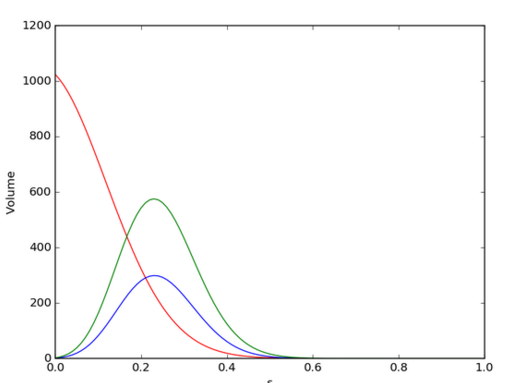
\includegraphics{pics/53.png}
 \caption{$s$-Volume}
 \label{fig:5.3}
\end{figure}

可以这样直观理解,exp指数贡献巨大,故此上式主要贡献在$A(s)=0.5$处取得此时,对于sigmoid来说,$s=0$,对于relu来说,$s=0.5$,这样根号里面的项对于sigmoid来说恒等于1,而对于relu来说,恒小于1。当输入n非常大的时候(100够大了),relu的积分贡献远小于sigmoid函数,或者说sigmoid函数的解空间远超relu。tanh也是远超过relu的.

sigmoid的好处并不是在训练上的,而是你的模型如果牵涉到许多概率问题,比如DBN,RNN,LSTM中的一些gate,就不能将sigmoid换成relu了,这样概率表达都错了。

relu型的,如上所述用于缓和饱和问题。而且还有部分缓和梯度衰减的作用,不像sigmoid一样,relu没有一个梯度衰减的尾巴,强度上不封顶。使得反向传播过程只有权值的乘积带来梯度的衰减。然而,一些网络可能需要clip 掉梯度,避免不封顶的爆炸梯度回传。

稀疏度问题,relu的稀疏机理同dropout机理不一样,dropout等效于动态L2规范带来的稀疏,是通过打压W 来实现稀疏的。relu稀疏是因为如果输入为零,输出也会为零,这样多层输入输出更加贴近于原始高维数据层的稀疏度,毕竟输入信息本来就是高度稀疏的。
\section{前馈神经网络}
\subsection{前馈计算}
\section{反向传播算法}
\section{梯度消失问题}

\section{训练方法}
\section{一些经验}
\section{进一步的阅读和总结}
%----------------------------------------------------------------------------------------
%	PART
%----------------------------------------------------------------------------------------

\part{经典网络 Classical Networks}

%----------------------------------------------------------------------------------------
%	CHAPTER 3
%----------------------------------------------------------------------------------------

\chapterimage{chapter_head_6.jpg}
\chapter{受限波尔兹曼机RBM}

Restricted Boltzmann Machines (RBMs) is a popular unsupervised method in Deep Learning Architectures. Despite its popularity, it takes efforts to grasp the concept. This post aims at providing an introduction to RBMs, from a somewhat mathematical point of view. Most of the formulas here are from\cite{bengio2009learning}.
\section{Roadmap}
Boltzmann Machines is an energy-based model where the joint probability distribution is characterized by a scalar energy to each configuration of variables. Boltzmann machine is also a probabilistic graphical model using graph-based representation as the basis for encoding the distribution. Restricted Boltzmann Machines is a type of Boltzmann machine with constrained connections – only a certain type of connection is allowed.

This post starts by introducing energy-based models, including the graphical representation of the model and its learning with gradient descent of log-likelihood. This post then discusses Boltzmann machines by placing a specific energy function in energy-based models. Restricted Boltzmann Machines are further discussed with the introduction of restrictions in Boltzmann Machines.
\section{Notations}
It is worthwhile to mention that there are three important notations in this post: $x$, $h$ and $y$. $x$ represents a list of input variables taking the form $x=\left \{ x_{1}, x_{2},\dots ,x_{N} \right \}$, where $x_{i}$ denotes the $i-th$ input variable. $h$ represents a list of hidden variables taking the form $h=\left \{ h_{1}, h_{2},\dots ,h_{N} \right \}$, where $h_{i}$ denotes the $i-th$ hidden variable. $y$ represents the label of a given input.

As an example, for the problem of image recognition, $x$ are the images of interest where $x_{i}$ are the individual pixels from an image $x$. $h$ are the $hidden features/descriptors$ that serve as a high-level representations of image. Finally, $y$ are the labels of the images.

\section{Energy-Based Models}
Different from $predictive/supervised$ models, such as back-propagation neural networks, energy-based models capture the joint probability distribution  $P(\mathbf{x})$  of the configuration of input variables $\left \{ x_{1}, x_{2},\dots ,x_{N} \right \}$, rather than conditional probability of $P(y|\mathbf{x})$ .

Energy-based models associate a scalar energy to each configuration of variables of interest. For each configuration, there is a corresponding energy associated with it, and this energy is directly associated with the probability for the model to be in this particular configuration. The probability distribution of energy-based models is defined as
\begin{equation}\label{add1.1}
    P(x)=\frac{e^{-Energy(x)}}{Z}
\end{equation}

This probability distribution favors “negative energy”, meaning configurations with low energy will have a high probability. Learning in energy-based models corresponds to modifying the energy function to reshape the energy space, so that the desired patterns in the model always lie in the lowest spots in the energy surface, so that it will have a high probability. RBMs is a form of Undirected Graphical Model which I will discuss in another post.
\section{An Simple Example of Energy-Based Models}
\begin{figure}[t]
 \centering
 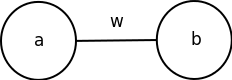
\includegraphics{pics/add1.png}
 \caption{An Simple Example of Energy-Based Models}
 \label{fig:add1}
\end{figure}
Suppose we have a simple energy-based model with only two variables $a$  and $b$  (where $x=\left \{ a, b \right \})$, as well as a connection weight $w$. Here we define energy function $Energy(a,b)=-wab$. If $a$ and $b$ can only take binary values, and $w$ is $1$, the resulting energy function takes the form $Energy(a,b)=-ab$. The table below shows all possible configurations for $a$, $b$, $Energy(a,b)$ and the probability for each configuration.
\begin{table}[htbp]
\
\begin{center}
  \caption{\label{tab:Energy}$Energy(a,b)$ and the probability for each configuration}
 \begin{tabular}{lclcl}
  \toprule
  $a$ & $b$ & $-Energy(a,b)$ & $e^{-Energy(a,b)}$ & $P(a,b)$ \\
  \midrule
 0 & 0 & 0& 1 & $\frac{1}{3+e}$\\
 0 & 1 & 0& 1 & $\frac{1}{3+e}$\\
 1 & 0 & 0& 1 & $\frac{1}{3+e}$\\
 1 & 1 & 1& e & $\frac{e}{3+e}$\\
  \bottomrule
 \end{tabular}
\end{center}

\end{table}

We can visualize the probability distribution using the graph below where the size of each circle represents the probability of each configuration.

\begin{figure}[t]
 \centering
 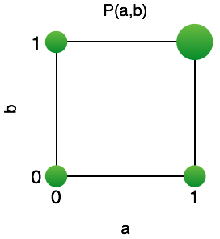
\includegraphics{pics/add2.png}
 \caption{Model}
 \label{fig:add2}
\end{figure}

\section{Introducing Hidden Variables}
When modelling a set of input features, we can use the input attributes as variables to learn the relationship between each other. However, directly modeling such variables seems to have less expressive power, hence, we introduce the concept of hidden variables (nonobserved variables), to better model the joint probability distribution. The hidden variables can be used to capture high level feature representations of the observed variables. The probability distribution and partition function are changed accordingly:
\begin{equation}\label{add1.2}
    P(\boldsymbol{x},\boldsymbol{h})=\frac{e^{-Energy(\boldsymbol{x},\boldsymbol{h})}}{Z}
\end{equation}
\begin{equation}\label{add1.3}
    Z=\sum_{\boldsymbol{x}}^{ }\sum_{\boldsymbol{h}}^{ }e^{-Energy(\boldsymbol{x},\boldsymbol{h})}
\end{equation}
Since we are only interested in the distribution of visible variables, we want to model the marginal distribution over hidden variables that takes the form

\begin{equation}\label{add1.4}
  P(\boldsymbol{x})=\sum_{\boldsymbol{h}}^{ }\frac{e^{-Energy(\boldsymbol{x},\boldsymbol{h})}}{Z}
\end{equation}

To simplify this formula, we defined free energy being the marginal energy of $x$ summing over $h$:
\begin{equation}\label{add1.5}
  FreeEnergy(\boldsymbol{x})=-ln\sum_{\boldsymbol{h}}^{ }e^{-Energy(\boldsymbol{x},\boldsymbol{h})}
\end{equation}
Therefore we can rewrite the marginal probability distribution as:

\begin{equation}\label{add1.6}
  P(\boldsymbol{x})=\frac{e^{-FreeEnergy(\boldsymbol{x})}}{Z}
\end{equation}
\begin{equation}\label{add1.7}
    Z=\sum_{x}e^{-FreeEnergy(\boldsymbol{x})}
\end{equation}
\section{Gradient Learning of Energy-based Models}
We use log-likelihood gradient to train the model, and we use $\theta$ to represent parameters of the model.
\begin{figure}[t]
 \centering
 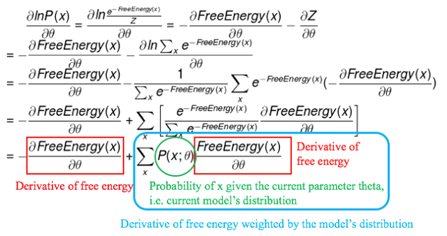
\includegraphics{pics/add3.png}
 \caption{Gradient Learning of Energy-based Models}
 \label{fig:add3}
\end{figure}

Hence, the average log-likelihood gradient for a training set is:
\begin{equation}\label{add1.8}
    E_{\hat{P}}\left[ \frac{\partial \ln P(\boldsymbol{x})}{\partial\theta} \right]=-E_{\hat{P}}\left[ \frac{\partial FreeEnergy(\boldsymbol{x})}{\partial\theta} \right]+E_{P}\left[ \frac{\partial FreeEnergy(\boldsymbol{x})}{\partial\theta} \right]
\end{equation}

where $\hat{P}$ is the distribution over the training set, and  $P$ is the distribution over the model's current parameters. The resulting log-likelihood gradient tells us, as long as we are able to compute the derivative of free energy for the training examples, and the derivative of free energy for the model's own distribution, we will be able to train the model tractably.
\section{Boltzmann Machines}
Boltzmann machine is a type of energy-based model, we get a Boltzmann machine when applying the energy function below in the previous section:
\begin{equation}\label{BME}
  Energy(\boldsymbol{x},\boldsymbol{h})=-\boldsymbol{b}^T\boldsymbol{x}-\boldsymbol{c}^T\boldsymbol{h}-\boldsymbol{h}^T\boldsymbol{Wx}-\boldsymbol{x}^T\boldsymbol{Ux}-\boldsymbol{h}^T\boldsymbol{Vh}
\end{equation}
where $b$ is the bias for visible variables, $c$ is the bias for hidden variables, $W$ is the connection weights between hidden variables and visible variables, $U$ is the connection weights within visible variables and $V$ is the connection weights within hidden variables. This energy function is simply a fully connected graph with weights on each connection.
\section{Gradient Learning of Boltzmann Machines}
The gradient of log-likelihood can be written as:
\begin{equation}\label{LLG}
  \frac{\partial \ln P(\boldsymbol{x})}{\partial \theta}=-\sum_{\boldsymbol{h}}P(\boldsymbol{x}\vert \boldsymbol{h})\frac{\partial Energy(\boldsymbol{x},\boldsymbol{h})}{\partial \theta} + \sum_{\tilde{\boldsymbol{x}},\boldsymbol{h}} P(\tilde{\boldsymbol{x}}, \boldsymbol{h})\frac{\partial Energy(\tilde{\boldsymbol{x}}, \boldsymbol{h})}{\partial \theta}
\end{equation}
Since the $\frac{\partial Energy(\boldsymbol{x},\boldsymbol{h})}{\partial \theta}$ is easy to compute (which is simply the connection weights), the result of this gradient tells us, as long as we are able to compute the probability of hidden variables given visible variables, and the joint probability of hidden and visible variables (for the current constraints in the model), we will be able to learn the model tractably. Now the question comes to, how to compute the conditional and joint probability. That is, how to sample from $P(\boldsymbol{x}\vert \boldsymbol{h})$ and $P(\boldsymbol{x},\boldsymbol{h})$.

\section{Gibbs Sampling for Conditional Probability}
Gibbs sampling of the joint distribution of $N$ variables $X_{1}...X_{N}$ is done through a sequence of $N$ sampling sub-steps of the form:
\begin{equation*}
  X_{i}\sim P(X_{i}|X_{-i}=x_{-i})
\end{equation*}

which means, the sample of one variable comes from the conditional probability given all other variables. We can compute the conditional probability of one node given all the other nodes easily:
\begin{gather*}
  P(h_i=1 \vert \boldsymbol{x}) \\
  ......=sigmoid(d_i+A^T_ix)
\end{gather*}

This conditional probability is the same form as the activation function of neural networks. In Gibbs sampling, one sample step is to sample all the $N$ variables once. After the number of sample steps goes to $\infty$, the sample distribution will converge to $P(X)$.
\section{Gibbs Sampling for Boltzmann Machines}
To sample $P(x\vert h)$ and $P(x,h)$ in Boltzmann machine, we need to compute two Gibbs chains. For $P(x\vert h)$, we clamp the visible nodes $(x)$ to sample $h$, which is the conditional probability. For $P(x,h)$, we let all the variables run free, to sample the distribution of the model itself. This method for training Boltzmann machine is computationally expensive, because we need to run two Gibbs chains, and each of them will need to run a large number of steps to get a good estimate of the probability. Now, we introduce the idea of Restricted Boltzmann Machine and how it speeds up learning.
\section{Restricted Boltzmann Machines}
Restricted Boltzmann machine is a type of Boltzmann machine, without interconnections within hidden nodes and visible nodes. The energy function is defined as
\begin{equation*}
  Energy(x,h)=-{b}^Tx-{c}^Th-{h}^TWx
\end{equation*}

The conditional probability of hidden variables given visible variables are:
\begin{gather*}
  P(h\vert x) \\
  ......=\prod_iP(h_i\vert x)
\end{gather*}
This conditional probability indicates the probability for each hidden variable given all the visible variables are independent, so that we can get the joint probability directly. This also indicates that, each hidden node can be seen as an expert, and we are using the \textbf{product of experts}\footnote{
\textbf{product of experts}(专家乘积模型??): To be simple, it means that $P(\boldsymbol{x})$ is able to written as the following form\cite{hinton2002training,welling2007product}:
\begin{gather*}
  P(\boldsymbol{x})=\sum_{\boldsymbol{h}}P(\boldsymbol{x},\boldsymbol{h})=\frac{1}{Z}\sum_{\boldsymbol{h}}\exp[-E(\boldsymbol{x},\boldsymbol{h})]\\
  =\frac{1}{Z}\sum_{\boldsymbol{h}}\exp[\sum_{i=1}^{n_x}b_ix_i+\sum_{j=1}^{n_h}c_jh_j+\sum_{i=1}^{n_x}\sum_{j=1}^{n_h}h_jw_{ji}x_i]\\
  =\frac{1}{Z}\sum_{h_1}\cdots\sum_{h_{n_h}}\exp[\sum_{i=1}^{n_x}b_ix_i+\sum_{j=1}^{n_h}c_jh_j+\sum_{i=1}^{n_x}\sum_{j=1}^{n_h}h_jw_{ji}x_i]\\
  =\frac{1}{Z}\sum_{h_1}\cdots\sum_{h_{n_h}}\exp(\sum_{i=1}^{n_x}b_ix_i)\exp[\sum_{j=1}^{n_h}h_j\cdot(c_j+\sum_{i=1}^{n_x}w_{ji}x_i)]\\
  =\frac{1}{Z}\exp(\sum_{i=1}^{n_x}b_ix_i)\sum_{h_1}\cdots\sum_{h_{n_h}}\prod_{j=1}^{n_h}\exp[h_j(c_j+\sum_{i=1}^{n_x}w_{ji}x_i)]\\
  =\frac{1}{Z}\exp(\sum_{i=1}^{n_x}b_ix_i)\sum_{h_1}\exp[h_1(c_1+\sum_{i=1}^{n_x}w_{1i}x_i)]\cdots\sum_{h_{n_h}}\exp[h_{n_h}(c_{n_h}+\sum_{i=1}^{n_x}w_{n_hi}x_i)]\\
  =\frac{1}{Z}\exp(\sum_{i=1}^{n_x}b_ix_i)\prod_{j=1}^{n_h}\sum_{h_j}\exp[h_j(c_j+\sum_{i=1}^{n_x}w_{ji}x_i)]\\
  =\frac{1}{Z}\prod_{i=1}^{n_x}\exp(b_ix_i)\prod_{j=1}^{n_h}\left(\exp[0\cdot(c_j+\sum_{i=1}^{n_x}w_{ji}x_i)]+\exp[1\cdot(c_j+\sum_{i=1}^{n_x}w_{ji}x_i)]\right)\\
  =\frac{1}{Z}\prod_{i=1}^{n_x}\exp(b_ix_i)\prod_{j=1}^{n_h}[1+\exp(c_j+\sum_{i=1}^{n_x}w_{ji}x_i)]\\
\end{gather*}
} to model the joint distribution. This formula also applies for $P(x\vert h)$.
\section{Gibbs Sampling for Restricted Boltzmann Machines}
For the Gibbs sampling in Boltzmann machine, it is very slow because we need to take a lot of sub-steps to get only one Gibbs chin. But for Restricted Boltzmann machine, since all the hidden variables are independent given visible variables and all the visible variables are independent given hidden variables, we can just take one step to complete one Gibbs chin. So that we can easily get the conditional probability. For the joint probability, we use a hybrid Monte-Carlo method, an MCMC method involving a number of free-energy gradient computation sub-steps for each step of the Markov chain. For $k$ Gibbs steps:
\begin{gather*}
  x_{0}\sim \hat{P}(x)\\
  h_{0}\sim P(h\vert x_{0})\\
  x_{1}\sim P(x\vert h_{0})\\
  h_{1}\sim P(h\vert x_{1})\\
  \dots \\
   x_{k} \sim P(x|h_{k-1})
\end{gather*}

\section{Contrastive Divergence}
Compared with the Gibbs sampling in Boltzmann machine, the above method to sample in Restricted Boltzmann machine is much more effective. However, runing the MCMC chain is still quite expensive. The idea of k-step Contrastive Divergence is to stop the MCMC chain after k steps. This method saved a lot of computational complexity. One way to interpret the Contrastive Divergence is that, after a few MCMC steps, we will know in which direction the error is heading towards, so that instead of waiting for the error becoming larger and larger, we can simply stop the chain the update the network.


The idea of k-step contrastive divergence learning (CD-k) is quite simple:Instead of approximating the second term in the log-likelihood gradient by a sample from the RBM-distribution (which would require to run a Markov chain until the stationary distribution is reached), a Gibbs chain is run for only $k$ steps (and usually $k=1$).The Gibbs chain is initialized with a training example  of the training set and yields the sample  after k steps. Each step t consists of sampling  from  and sampling  from  subsequently.The gradient w.r.t.  of the log-likelihood for one training pattern  is then approximated by:
\begin{equation}\label{CDk}
  CD_k(\bold{\theta},\bold{x}^{(0)})=-\sum_{\bold{h}}p(\bold{h}|\bold{x}^{(0)})
\frac{\partial E(\bold{x}^{(0)},\bold{h})}
{\partial \bold{\theta}}
+
\sum_{\bold{h}}p(\bold{h}|\bold{x}^{(k)})
\frac{\partial E(\bold{x}^{(k)},\bold{h})}
{\partial \bold{\theta}}
\end{equation}
首先,那个Sampling,就是:

sample  $h_i^{(t)} \sim   p(h_i|\bold{x}^{(t)})$

sample $x_j^{(t+1)} \sim p(x_j|\bold{h}^{(t)})$


这个sample是这样的\footnote{详见http://blog.csdn.net/itplus/article/details/19408143}:首先,我们的$h_i$ 只会取$0$或者$1$ 两个状态,为了方便起见,这里按照进行采样,那么在采样的时候遵循以下步骤:
\begin{enumerate}
  \item 计算$p(h_i = 1|\bold{x}^{(t)})$,得到的概率值,记为$p$
  \item 生成一个$[0,1)$的随机数,记为$p^*$
  \item 如果$p^* < p$,则$h_i^{(t)}=1$,反之为$0$
\end{enumerate}

对$x_j^{(t+1)}$的采样也是一样。

\begin{algorithm}[H]
 \KwData{$RBM(X_1,...,X_m,H_1,...,H_n)$, training batch $S$}
 \KwResult{Gradient Approximation $\Delta w_{ij}$, $\Delta b_j$ and $\Delta c_i$ for $i=1,...,n$ and $j=1,...,m$}
 %initialization\;
 \ForAll{the $\bold{x} \in S$}{
  $\bold{x}^{(0)} \leftarrow \bold{x}$\;
  	\For {$t = 0, ..., k - 1$}{
		\For {$i = 1, ..., n$}{
              sample $h_t^{(t)} \sim p(h_i|\bold{x}^{(t)})$\;
              .\;
              .\;}}
        \For {$j = 1, ..., m$}{
              sample $x_j^{(t+1)} \sim p(x_j|\bold{h}^{(t)})$\;
		.\;
		.\;}
	\For {$i = 1,...,n$}{
		\For {$j = 1,..., m$}{
			$\Delta w_{ij} \leftarrow \Delta w_{ij} + p(H_i = 1 | \bold{x} ^{(0)}) \cdot x_j^{(0)} - p(H_i = 1 | \bold{x}^{(k)}) \cdot x_j^{(k)}$\;}}
	\For {$j = 1, ..., m$}{
			$\Delta b_{j} \leftarrow \Delta b_j + x_j^{(0)} - x_j^{(k)}$\;}
	\For {$i = 1, ..., n$}{
			$\Delta c_{i} \leftarrow \Delta c_{i} + p (H_i = 1 | \bold{x}^{(0)}) - p(H_i = 1 \bold{x}^{(k)})$\;}

 }
 \caption{k-step contrastive divergence}
\end{algorithm}
\section{Gibbs Sampling和Markov Chain以及MCMC的关系}
首先,Gibbs Sampling是根据邻居的状态进行采样的,Gibbs Sampling是沿着转移矩阵$P=\{p_{xy}\}$ 进行转移的,这就是为什么一次只转移一个轴(一次只采样一个变量)。而之前的MCMC那一坨东西只是为了说明,对于我们的Gibbs Distribution $p(\bold{h},\bold{x})=\frac{1}{Z}e^{-E(\bold{h},\bold{x})}$ ,总会存在一个Transition Matrix P,使得$p$ 为其stationary distribution (是否收敛于stationary distribution 取决于转移矩阵Transition Matrix)。而这个Transition Matrix的构造以此证明了这一点—— 对RMBs这种图拓扑结构来说,总会存在一个Transition Matrix P(这里的这个P是个矩阵),使得概率函数$p$ 为其stationary distribution。 因此我们按照Transition Matrix 中的Transition Probability做转移,才可以得到符合分布的一个样本\footnote{https://en.wikipedia.org/wiki/Gibbs\_sampling}。Gibbs Sampling是沿着Markov Chain做转移\footnote{详见http://www.52nlp.cn/lda-math-mcmc-\%E5\%92\%8C-gibbs-sampling2},请好好体会一下这句话。


\section{CD Algorithm是如何对原来的分布$p$ 进行优化的}
首先,根据$\bold{x}^{(0)}$对$\bold{h}^{(0)}$进行采样,然后根据$\ bold{h}^{(0)}$ 对$\bold{x}^{(1)}$进行采样,这样就保证了“采样-拟合-再采样-再他妈拟合”—— 对于CD-1 来说这个过程只有“采样- 拟合”。

换言之,对$\bold{x}^{(0)}$来说,$\bold{h}^{(0)}$ 会使得分布函数变成更符合$\bold{x}^{(0)}$ 的情况,而不是状态初始时的$\bold{h}^{*}$($\bold{h}$ 是随机初始化的,具体见文献\footnote{详见https://www.cs.toronto.edu/~hinton/absps/guideTR.pdf Section 3})。

然后根据$\bold{h}^{(0)}$生成的样本$\bold{x}^{(1)}$又会使得联合分布函数在上表现得更好。

联合分布函数是在针对$\bold{h}^{(0)}$的采样和对$\ bold{x}^{(k)}$的拟合中不断变好的。

因为随着对$\bold{h}^{(0)}$的采样,联合分布函数$p$会改变,因为对应energy function 里的$\bold{h}$ 变了($\bold{h}$的每一个分量在采出$\ bold{h}^{(0)}$分量$h_j^{(0)}$的样本时,对应分量$h_j$就会变为$h_j^{(0)} $的取值\footnote{详见https://www.cs.toronto.edu/~hinton/absps/guideTR.pdf})。


而$\bold{x}^{(k)}$的拟合中,虽然没有直接改变联合分布函数$p$,但是接下来的花样梯度近似大赛中,联合分布函数$p$ 会改变。

换言之,对联合分布函数$p$的改善来源于根据真实数据$\bold{x}^{(0)}$拟合出的比之前$\bold{h}$更合理的$\bold{h}^{(0)}$

根据更合理的$\bold{h}^{(0)}$采样出的近似真实数据$\bold{x}^{(k)}$的拟合—— 这个拟合体现在梯度的近似上。一点一点概率函数就被修改的更好了。

这TM肯定有详细的数学证明但是我看不动了以后再说。
%---------------------------------------------
\chapterimage{chapter_head_7.jpg}
\chapter{卷积神经网络CNN}
\textbf{卷积神经网络}(Convolutional Neural Networks,CNN)是一种前馈神经网络。卷积神经网络是受生物学上\textbf{感受域}(Receptive Field)的机制而提出的。感受野主要是指听觉系统、本体感觉系统和视觉系统中神经元的一些性质。比如在视觉神经系统中,一个神经元的感受野是指视网膜上的特定区域,只有这个区域内的刺激才能够激活该神经元\cite{hubel1968receptive}。

卷积神经网络有三个结构上的特性:局部连接,权重共享以及空间或时间上的次采样。这些特性使得卷积神经网络具有一定程度上的平移、缩放和扭曲不变性\cite{lecun1998gradient}。
\section{卷积}
\textbf{卷积},也称褶积,是数学分析中的一种重要运算,这里只考虑离散序列的情况。

\subsection{一维场合}
一维卷积经常用在信号处理中。给定一个输入信号序列$x_t, t = 1,\cdots, n$,和滤波器$f_t, t = 1,\cdots,m$,一般情况下滤波器的长度$m$远小于信号序列长度$n$。

卷积的输出为:
\begin{equation}\label{6.1}
  y_t=\sum_{k=1}^n{f_k\cdot x_{t-k+1}}
\end{equation}

当滤波器$f_t=1/n$ 时,卷积相当于信号序列的移动平均。

卷积的结果按输出长度不同可以分为两类:一类是\textbf{宽卷积},输出长度$n+m-1$,对于不在$[1,n]$ 范围之外的$x_t$ 用零补齐(zero-padding)。一类是\textbf{窄卷积},输出长度$n-m+1$,不补零。

在这里除了特别声明,我们一般说的卷积默认为\textbf{窄卷积}。

\subsection{二维场合}
一维卷积经常用在图像处理中。给定一个图像$x_{ij}, 1 \leq i \leq M, 1 \leq j \leq N$,和滤波器$f_{ij}, 1 \leq i \leq m, 1 \leq j \leq n$,一般$m \ll M, n \ll N$。

卷积的输出为:
\begin{equation}\label{6.2}
  y_{ij}=\sum_{u-1}^m\sum_{v=1}^n{f_{uv}\cdot x_{i-u+1,j-v+1}}
\end{equation}

在图像处理中,常用的均值滤波(mean filter)就是当前位置的像素值设为滤波器窗口中所有像素的平均值,也就是$f_{uv} = 1/mn$。

\section{卷积层:用卷积代替全链接}
\begin{figure}[t]
 \centering
 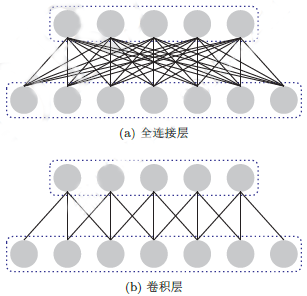
\includegraphics{pics/61.png}
 \caption{Full Connection Layer and Convolutional Layer}
 \label{fig:6.1}
\end{figure}

在全连接前馈神经网络中,如果第$l $层有$n^l$个神经元,第$l-1$ 层有$n^{(l-1)}$个神经元,连接边有$n^{(l)}\cdot n^{(l-1)}$ 个,也就是权重矩阵有$n^{(l)}\cdot n^{(l-1)}$ 个参数。当$m$和$n$ 都很大时,权重矩阵的参数非常多,训练的效率会非常低。

如果采用卷积来代替全连接,第$l$层的每一个神经元都只和第$l-1$ 层的一个局部窗口内的神经元相连,构成一个局部连接网络。第$l$层的第$i$个神经元的输入定义为:
\begin{gather}\label{6.2}
  a_i^{(l)}=f\left( \sum_{j-1}^{(l)}{w_j^{(l-1)}\cdot a_{i-j+m}^{(l-1)}}+b^{(l)} \right) \\
  =f\left( \boldsymbol{w}^{(l)}\cdot \boldsymbol{a}_{(i+m-1):i}^{(l-1)}+b_i \right)
\end{gather}
其中,$\boldsymbol{w}^{(l)}\in \mathbb{R}^m$为$m$维的滤波器,$\boldsymbol{a}_{(i+m-1):i}^{(l)}=[a_{(i+m-1)}^{(l)},\cdots ,a_{i}^{(l)}]^T$。 这里$a^{(l)}$的下标从1 开始,这里的卷积公式和原始的公式中的$\boldsymbol{a}$的下标有所不同。

上述公式也可以写成:
\begin{equation}\label{6.5}
  \boldsymbol{a}^{(l)}=f(\boldsymbol{w}^{(l)}\otimes \boldsymbol{a}^{(l-1)}+b^{(l)})
\end{equation}
$\otimes$表示卷积运算。

从式\ref{6.5}可知,$\boldsymbol{w}^{(l)}$ 对所有神经元是相同的。这也是卷积层的灵位一个特性:\textbf{权值共享}。这样,在卷积层中,只需$m+1$个参数。另外,第$l+1$层的神经元个数不是任意选择的,而是满足$n^{(l+1)}=n^{(l)}-m+1$。

上面是一维卷积层的情况,下面考察二维的情况。在图像处理中,图象是以二维矩阵的形式输入到神经网络中,因此,假设$x^{(l)}\in \mathbb{R}^{(w_l\cdot h_l )}$ 和$ ^{(l-1)}\in \mathbb{R}^{(w_{l-1}\cdot h_{l-1})}$分别是第$l$层和第$l-1$层的神经元活性。$X^{(l)}$的每一个元素为:
\begin{equation}\label{6.6}
  X_{s,t}^{(l)}=f\left( \sum_{i=1}^u \sum_{j=1}^n{W_{i,j}^{(l)}\cdot X_{s-i+u,t-j+v}^{(l-1)}+b^{(l)}} \right)
\end{equation}
其中,$W^{(l)}\in \mathbb{R}^{u \times v}$ 为二维的滤波器,$b$ 为偏置矩阵。第$l-1$层的神经元个数为$(w_l\times h_l)$,并且$w_l=w_{l-1}-u+1, h_l=h_{l-1}-v+1$。

于是上式也可以写为:
\begin{equation}\label{6.7}
  X^{(l)}=f\left( W^{(l)} \otimes X^{(l-1)} +b^{(l)} \right)
\end{equation}

为了增强卷积层的表示能力,我们可以使用$K$ 个不同的滤波器来得到$K$组输出。每一组输出都共享一个滤波器。如果我们把滤波器看成一个特征提取器,每一组输出都可以看成是输入图像经过一个特征抽取后得到的特征。因此,在卷积神经网络中每一组输出也叫作一组\textbf{特征映射}(Feature Map)。

不失一般性,假设第$l-1$层的特征映射组数为$n_{l-1}$,每组特征映射的大小为$m_{l-1}=w_{l-1}\times h_{l-1}$。 第$l-1$层的神经元数:$n_{l-1}\times m_{l-1}$。 第$l$ 层的特征映射组数为$n_l$。 如果假设第$l$ 层的每一组特征映射$X^{(l,k)}$的输入为第$l-1$ 层的所有特征映射组。

\begin{figure}[t]
 \centering
 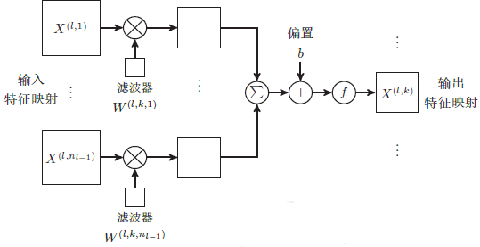
\includegraphics{pics/62.png}
 \caption{The mapping relationship of 2-D convolutional layer}
 \label{fig:6.2}
\end{figure}

第$l$层的第$k$组特征映射$X^{(l,k)}$为:
\begin{equation}\label{6.8}
  X^{(l,k)}=f\left( \sum_{p=1}^{n_l-1}(W^{(l,k,p)} \otimes X^{(l-1,p)})+b^{(l,k)} \right)
\end{equation}
其中,$W^{(l,k,p)}$表示第$l-1$层的第$p$组特征向量到第$l$层的第$k$组特征映射所需要的滤波器。

第$l$层的每一组特征映射都需要$n_{l-1}$个滤波器以及一个偏置$b$。假设每个滤波器的大小为$u \times v$,那么共需要$n_l \times n_{l-1} \times (u \times v) + n_l$。

这样,我们在第$l+1$层就得到$n_l$组特征映射,每一组特征映射的大小为$m_l = w_{l-1}-u+1\times h_{l-1}-v +1$,总的神经元个数为$n_l \times m_l$。 图\ref{fig:6.2} 给出了式\ref{6.8}的可视化映射关系。

\textbf{连接表}:  式\ref{6.8}中,第$l-1$ 层的所有特征映射都经过滤波器得到一个第$l$ 层的一组特征映射$X^{(l,k)}$。也就是说,第$l$ 层的每一组特征映射都依赖于第$l$ 层的所有特征映射,相当于不同层的特征映射之间是全连接的关系。实际上,这种全连接关系不是必须的。我们可以让第$l$ 层的每一组特征映射都依赖于前一层的少数几组特征映射。这样,我们定义一个\textbf{连接表}$T$ 来描述不同层的特征映射之间的连接关系。如果第$l$ 层的第$k$ 组特征映射依赖于前一层的第$p$ 组特征映射,则$T_{p,k}=1$,否则为$0$。
\begin{equation}\label{6.9}
  X^{(l,k)}=f\left( \sum_{p=1, T_{p,k}=1}(W^{(l,k,p)} \otimes X^{(l-1,p)})+b^{(l,k)} \right)
\end{equation}
\begin{figure}[t]
 \centering
 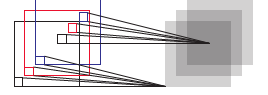
\includegraphics{pics/63.png}
 \caption{2-D convolutional layer}
 \label{fig:6.3}
\end{figure}

这样,假如连接表$T$的非零个数为$K$,每个滤波器的大小为$u \times v$,那么共需要$K \times (u \times  v) + n_l$ 参数。

卷积层的作用是提取一个局部区域的特征,每一个滤波器相当于一个特征提取器。图\ref{fig:6.3}给出了两维卷积层示例。
\section{子采样层:池化}

卷积层虽然可以显著减少连接的个数,但是每一个特征映射的神经元个数并没有显著减少。这样,如果后面接一个分类器,分类器的输入维数依然很高,很容易出现过拟合。为了解决这个问题,在卷积神经网络一般会在卷积层之后再加上一个池化(Pooling)操作,也就是子采样(Subsampling),构成一个子采样层。子采样层可以来大大降低特征
的维数,避免过拟合。

对于卷积层得到的一个特征映射$X^{(l)}$,我们可以将$X^{(l)}$划分为很多区域$R_k, k=1,\cdots ,K$,这些区域可以重叠,可以不重叠。一个子采样函数$\boldsymbol{down}(\cdot)$定义为:
\begin{gather}\label{6.10}
  X_k^{(l+1)}=f(Z_k^{(l+1)}) \\
  =f\left( w^{(l+1)}\cdot \boldsymbol{down}(R_k) + b^{(l+1)} \right)
\end{gather}
其中,$w^{(l+1)}$和$b^{(l+1)}$分别是可训练的权重和偏置参数。

\begin{gather}\label{6.12}
  X^{(l+1)}=f(Z^{(l+1)}) \\
  =f\left( w^{(l+1)}\cdot \boldsymbol{down}(X^l) + b^{(l+1)} \right)
\end{gather}
$\boldsymbol{down}(X^l)$是指子采样后的特征映射。

子采样函数$\boldsymbol{down}(\cdot)$一般是取区域内所有神经元的最大值(Maximum Pooling)或平均值(Average Pooling)。
\begin{equation}\label{6.14}
  pool_{max}(R_k)=max_{i\in R_k}a_i
\end{equation}
\begin{equation}\label{6.15}
  pool_{avg}(R_k)=\frac{1}{|R_k|}\sum_{i\in R_k}a_i
\end{equation}

子采样的作用还在于可以使得下一层的神经元对一些小的形态改变保持不变性,并拥有更大的感受域。
\section{CNN示例:LeNet-5}
下面我们来看一个具体的深层卷积神经网络:LeNet-5\cite{lecun1998gradient}。LeNet-5 虽然提出时间比较早,但是是一个非常成功的神经网络模型。基于LeNet-5 的手写数字(MNIST) 识别系统在90 年代被美国很多银行使用,用来识别支票上面的手写数字。LeNet-5 的网络结构如图\ref{fig:6.4}所示。
\begin{figure}[t]
 \centering
 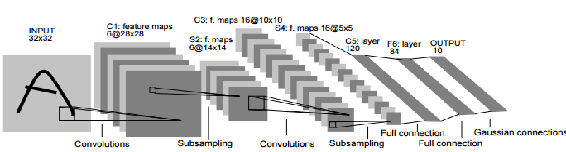
\includegraphics{pics/64.png}
 \caption{Net Structure of LeNet-5}
 \label{fig:6.4}
\end{figure}
\begin{figure}[t]
 \centering
 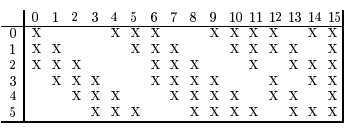
\includegraphics{pics/65.png}
 \caption{Connection table of LeNet-5's C3 layer}
 \label{fig:6.5}
\end{figure}
不计输入层,LeNet-5 共有7 层,每一层的结构为:
\begin{enumerate}
  \item 输入层:输入图像大小为$32 \times 32 = 1024$。
  \item C1层:这一层是卷积层。滤波器的大小是$5\times 5 = 25$,共有$6$个滤波器。得到$6$组大小为$28 \times 28 = 784$的特征映射。因此,C1层的神经元个数为$6 \times 784 = 4704$。 可训练参数个数为$6 \times 25 + 6 = 156$。连接数为$156 \times 784 = 122304$ (包括偏置在内,下同)。
  \item S2 层:这一层为子采样层。由C1层每组特征映射中的$2\times 2$ 邻域点次采样为$1$ 个点,也就是$4$ 个数的平均。这一层的神经元个数为$14 \times 14 = 196$。 可训练参数个数为$6 \times (1 + 1) = 12$。连接数为$6 \times 196 \times (4 + 1) = 122304$ (包括偏置的连接)
  \item C3 层:这一层是卷积层。由于S2 层也有多组特征映射,需要一个连接表来定义不同层特征映射之间的依赖关系。LeNet-5 的连接表如图\ref{fig:6.5} 所示。这样的连接机制的基本假设是:C3层的最开始的$6$个特征映射依赖于S2层的特征映射的每$3$个连续子集。接下来的$6$个特征映射依赖于S2 层的特征映射的每$4$ 个连续子集。再接下来的3 个特征映射依赖于S2层的特征映射的每$4$个不连续子集。最后一个特征映射依赖于S2 层的所有特征映射。这样共有$60$ 个滤波器,大小是$5 \times 5 = 25$。得到$16$组大小为$10\times 10 = 100$ 的特征映射。C3 层的神经元个数为$16 \times 100 = 1600$。 可训练参数个数为$60 \times 25 + 16 = 1516$。 连接数为$1516 \times 100 = 151600$。
  \item S4 层:这一层是一个子采样层,由$2\times 2$邻域点次采样为$1$ 个点,得到$16$组$5\times 5$大小的特征映射。可训练参数个数为$16 \times 2 = 32$。连接数为$16 \times (4 + 1) = 2000$。
  \item C5 层:是一个卷积层,得到$120$组大小为$1 \times 1$的特征映射。每个特征映射与S4 层的全部特征映射相连。有$120 \times 16 = 1920$ 个滤波器,大小是$5 \times 5 = 25$。C5 层的神经元个数为$120$,可训练参数个数为$1920 \times 25 + 120 = 48120$。 连接数为$120 \times (16 \times 25+1)=48120$
  \item F6层:是一个全连接层,有$84$个神经元,可训练参数个数为$84\times (120+1) = 10164$。 连接数和可训练参数个数相同,为$10164$。
  \item 输出层:输出层由10 个欧氏径向基函数(Radial Basis Function,RBF)函数组成。这里不再详述。
\end{enumerate}


\section{梯度计算}
在全连接前馈神经网络中,目标函数关于第$l$ 层的神经元$z^{(l)}$的梯度为:
\begin{gather}\label{6.16}
  \delta ^{(l)}\equiv \frac{\partial J(W,\boldsymbol{b};\boldsymbol{x},y)}{\partial \boldsymbol{z}^{(l)}} \\
  =f'_l(\boldsymbol{z}^{(l)})\odot (W^{(l+1)})^T\delta^{(l+1)}
\end{gather}

在卷积神经网络中,每一个卷积层后都接着一个子采样层,然后不断重复。因此需要分别来看下卷积层和子采样层的梯度。
\subsection{卷积层的梯度}
我们假定卷积层为$l$层,子采样层为$l + 1$ 层。因为子采样层是下采样操作,$l + 1$层的一个神经元的误差项$\delta$对应于卷积层(上一层)的相应特征映射的一个区域。$l$层的第$k$个特征映射中的每个神经元都有一条边和$l + 1$层的第$k$ 个特征映射中的一个神经元相连。根据链式法则,第$l$ 层的一个特征映射的误差项$\delta^{(l,k)}$,只需要将$l + 1$层对应特征映射的误差项$\delta^{(l+1,k)}$ 进行上采样操作(和第$l$层的大小一样),再和$l$ 层特征映射的激活值偏导数逐元素相乘,再乘上权重$w^{(l+1,k))}$,就得到了$\delta^{(l,k)}$。

第$l$层的第$k$个特征映射的误差项$\delta^{(l,k)}$ 的具体推导过程如下:
\begin{gather}\label{6.18}
  \delta^{(l,k)} \equiv \frac{\partial J(W,\boldsymbol{b};\boldsymbol{x},y)}{\partial Z^{(l)}}\\
  =\frac{\partial X^{(l,k)}}{\partial Z^{(l,k)}}\cdot \frac{\partial X^{(l+1,k)}}{\partial Z^{(l,k)}}\cdot\frac{\partial J(W,\boldsymbol{b};X,y)}{\partial Z^{(l+1,k)}}\\
  =f'_l(\boldsymbol{z}^{(l)})\odot \left( \boldsymbol{up}(w^{(l+1,k)}\delta^{(l+1)}) \right)\\
  =w^{(l+1,k)}\left( f'_l(\boldsymbol{z}^{(l)}) \odot \boldsymbol{up}(\delta^{(l+1)}) \right)
\end{gather}
其中,$\boldsymbol{up}$为上采样函数(Upsampling)。

在得到第$l$层的第$k$个特征映射的误差项$\delta^{(l,k)}$,目标函数关于第$l$层的第$k$个特征映射神经元滤波器$W_{i,j}^{(l,k,p)}$ 的梯度:
\begin{gather}\label{6.22}
  \frac{\partial J(W,\boldsymbol{b};\boldsymbol{x},y)}{\partial W_{i,j}^{(l,k)}} = \sum_{s=1}^{w_l}\sum_{t=1}^{h_j} \left( X_{s-i+u,t-j+v}^{(l-1,p)}\cdot(\delta^{(l,k)})_{s,t}\right)\\
  =\sum_{s=1}^{w_l}\sum_{t=1}^{h_j} \left( X_{s-i+u,t-j+v}^{(l-1,p)}\cdot(\boldsymbol{rot180}(\delta^{(l,k)}))_{s,t}\right)
\end{gather}

式\ref{6.22}也刚好是卷积形式,因此目标函数关于第$l$层的第$k$个特征映射神经元滤波器$W^{(l,k,p)}$ 的梯度可以写为:
\begin{equation}\label{6.24}
  \frac{\partial J(W,\boldsymbol{b};\boldsymbol{x},y)}{\partial W_{i,j}^{(l,k)}}=\boldsymbol{rot180}\left(  X^{(l-1,p)}\otimes \boldsymbol{rot180}((\delta^{(l,k)}))_{s,t}) \right)
\end{equation}

目标函数关于第$l$层的第$k$个特征映射的偏置$b^{(l)}$的梯度可以写为:
\begin{equation}\label{6.25}
  \frac{\partial J(W,\boldsymbol{b};\boldsymbol{x},y)}{\partial b^{(l,k)}}=\sum_{i,j}(\delta^{(l,k)})_{i,j}
\end{equation}
\subsection{子采样层的梯度}
我们假定子采样层为$l$层,$l+1$层为卷积层。因为子采样层是下采样操作,$l+1$层的一个神经元的误差项$\delta$ 对应于卷积层(上一层)的相应特征映射的一个区域。
\begin{equation}\label{6.26}
  X^{(l+1,k)}=\sum_{p,T_{p,k}=1}(W^{(l+1,k,p)}\otimes X^{(l,p)})+b^{(l+1,k)}
\end{equation}

第$l$层的第$k$个特征映射的误差项$\delta^{(l,k)}$ 的具体推导过程如下:
\begin{gather}\label{6.27}
  \delta^{(l,k)} \equiv \frac{\partial J(W,\boldsymbol{b};X,y)}{\partial Z^{(l,k)}}\\
  =\frac{\partial X^{(l,k)}}{\partial Z^{(l,k)}}\cdot \frac{\partial X^{(l+1,k)}}{\partial Z^{(l,k)}}\cdot\frac{\partial J(W,\boldsymbol{b};X,y)}{\partial Z^{(l+1,k)}}\\
  =f'_l(\boldsymbol{z}^{(l)})\odot\left( \sum_{p,T_{p,k}=1}(\delta^{(l+1,p)}\widetilde{\otimes}\boldsymbol{rot180}(W^{(l,k,p)})) \right)
\end{gather}
其中,$\widetilde{\otimes}$为宽卷积。

式\ref{6.22}也刚好是卷积形式,因此目标函数关于第$l$层的第$k$个特征映射神经元滤波器$W^{(l,k,p)}$ 的梯度可以写为:
\begin{equation}\label{6.30}
  \frac{\partial J(W,\boldsymbol{b};X,y)}{\partial w^{(l,k)}}=\sum_{i,j}\left( \boldsymbol{down}(X^{(l-1,k)}\cdot \delta^{(l,k)}) \right)_{i,j}
\end{equation}

目标函数关于第$l$层的第$k$个特征映射的偏置$b^{(l)}$的梯度可以写为
\begin{equation}\label{6.31}
  \frac{\partial J(W,\boldsymbol{b};X,y)}{\partial b^{(l,k)}}=\sum_{i,j}(\delta^{(l.k)})_{i,j}
\end{equation}
\section{一个强大的CNN框架:CAFFE}
Caffe,全称Convolutional Architecture for Fast Feature Embedding,是一个计算CNN相关算法的框架,并具有结构清晰,可读性高,运行快速的特点,http://caffe.berkeleyvision.org/。
\subsection{Caffe的特点}
  \subsubsection{Caffe相对与其他DL框架的优点和缺点}

优点:
  \begin{itemize}
    \item 速度快。Google Protocol Buffer 数据标准为Caffe提升了效率。
    \item 学术论文采用此模型较多。不确定是不是最多,但接触到的不少论文都与Caffe 有关(R-CNN,DSN,最近还有人用Caffe实现LSTM)。
  \end{itemize}
缺点:
\begin{itemize}
  \item 曾更新过重要函数接口。偶尔会出现接口变换的情况,很久前写的代码可能过了一段时间就不能和新版本很好地兼容。(现在更新速度放缓,接口逐步趋于稳定)。
  \item 对于某些研究方向来说的人并不适合。这个需要对Caffe的结构有一定了解,(后面提到)。
\end{itemize}
\subsubsection{Caffe代码层次}
学习Caffe需要从熟悉Blob,Layer,Net,Solver这样的几大类这个顺序开始学习的,这四个类复杂性从低到高,贯穿了整个Caffe。 把他们分为三个层次介绍:
\begin{itemize}
  \item Blob:是基础的数据结构,是用来保存学习到的参数以及网络传输过程中产生数据的类。
  \item Layer:是网络的基本单元,由此派生出了各种层类。修改这部分的人主要是研究特征表达方向的。
  \item Net:是网络的搭建,将Layer 所派生出层类组合成网络;
  \item Solver:是Net 的求解,修改这部分人主要会是研究DL 求解方向的。
\end{itemize}
\subsection{更进一步的特点}
\subsubsection{Blob}
Caffe支持CUDA,在数据级别上也做了一些优化,这部分最重要的是知道它主要是对protocol buffer所定义的数据结构的继承,Caffe也因此可以在尽可能小的内存占用下获得很高的效率。(追求性能的同时Caffe 也牺牲了一些代码可读性)
在更高一级的Layer中Blob用下面的形式表示学习到的参数:
\lstset{language=C++}
\begin{lstlisting}[frame=single]
vector<shared_ptr<Blob<Dtype> > > blobs_;

\end{lstlisting}

这里使用的是一个Blob的容器是因为某些Layer 包含多组学习参数,比如多个卷积核的卷积层。以及Layer 所传递的数据形式,后面还会涉及到这里:
\lstset{language=C++}
\begin{lstlisting}[frame=single]  % Start your code-block

vector<Blob<Dtype>*> &bottom;
vector<Blob<Dtype>*> *top;

\end{lstlisting}
\subsubsection{Layer}

 \textbf{Layer的五个派生类型}

Caffe十分强调网络的层次性,也就是说卷积操作,非线性变换(ReLU 等),Pooling,权值连接等全部都由某一种Layer 来表示。具体来说分为5大类Layer:
\begin{itemize}
  \item \textbf{NeuronLayer}类 定义于neuron\_layers.hpp中,其派生类主要是元素级别的运算(比如Dropout 运算,激活函数ReLu,Sigmoid等),运算均为同址计算(in-place computation,返回值覆盖原值而占用新的内存)。
  \item \textbf{LossLayer类} 定义于loss\_layers.hpp中,其派生类会产生loss,只有这些层能够产生loss。
  \item \textbf{数据层} 定义于data\_layer.hpp 中,作为网络的最底层,主要实现数据格式的转换。
  \item \textbf{特征表达层} 定义于vision\_layers.hpp (为什么叫vision 这个名字,我目前还不清楚),实现特征表达功能,更具体地说包含卷积操作,Pooling操作,他们基本都会产生新的内存占用(Pooling相对较小)。
  \item \textbf{网络连接层和激活函数} 定义于common\_layers.hpp,Caffe提供了单个层与多个层的连接,并在这个头文件中声明。这里还包括了常用的全连接层InnerProductLayer 类。
\end{itemize}

\textbf{Layer的重要成员函数}

在Layer内部,数据主要有两种传递方式,正向传导(Forward)和反向传导(Backward)。Forward和Backward有CPU和GPU(部分有)两种实现。Caffe中所有的Layer都要用这两种方法传递数据。
\lstset{language=C++}
\begin{lstlisting}[frame=single]  % Start your code-block

virtual void Forward(const vector<Blob<Dtype>*> &bottom,
                     vector<Blob<Dtype>*> *top) = 0;
virtual void Backward(const vector<Blob<Dtype>*> &top,
                      const vector<bool> &propagate_down,
                      vector<Blob<Dtype>*> *bottom) = 0;

\end{lstlisting}

Layer类派生出来的层类通过这实现这两个虚函数,产生了各式各样功能的层类。Forward是从根据bottom计算top的过程,Backward则相反(根据top计算bottom)。注意这里为什么用了一个包含Blob的容器(vector),对于大多数Layer来说输入和输出都各连接只有一个Layer,然而对于某些Layer存在一对多的情况,比如LossLayer和某些连接层。在网路结构定义文件(*.proto)中每一层的参数bottom 和top 数目就决定了vector中元素数目。

layers \{

  bottom: "decode1neuron"   // The first layer subconnected to this;

  bottom: "flatdata"        // The second layer subconnected to this;

  top: "l2\_error"           // The first layer upconnected to this;

  name: "loss"              // Name of this layer;

  type: EUCLIDEAN\_LOSS      // Type of this layer;

  loss\_weight: 0

\}
\\

\textbf{Layer的重要成员变量}

\textbf{loss}
\lstset{language=C++}
\begin{lstlisting}[frame=single]  % Start your code-block

vector<Dtype> loss_;

\end{lstlisting}
每一层又有一个loss\_值,只不多大多数Layer 都是0,只有LossLayer才可能产生非0的loss\_。计算loss 是会把所有层的loss\_相加

\textbf{learnable parameters}
\lstset{language=C++}
\begin{lstlisting}[frame=single]  % Start your code-block

vector<shared_ptr<Blob<Dtype> > > blobs_;

\end{lstlisting}
Layer学习到的参数。

\subsubsection{Net}
Net用容器的形式将多个Layer有序地放在一起,其自身实现的功能主要是对逐层Layer进行初始化,以及提供Update( )的接口(更新网络参数),本身不能对参数进行有效地学习过程。
\lstset{language=C++}
\begin{lstlisting}[frame=single]  % Start your code-block

vector<shared_ptr<Layer<Dtype> > > layers_;

\end{lstlisting}
同样Net也有它自己的:
\lstset{language=C++}
\begin{lstlisting}[frame=single]  % Start your code-block

vector<Blob<Dtype>*>& Forward(const vector<Blob<Dtype>* > & bottom,Dtype* loss = NULL);
void Net<Dtype>::Backward();

\end{lstlisting}
他们是对整个网络的前向和方向传导,各调用一次就可以计算出网络的loss。
\subsubsection{Solver}
这个类中包含一个Net的指针,主要是实现了训练模型参数所采用的优化算法,它所派生的类就可以对整个网络进行训练了。
\lstset{language=C++}
\begin{lstlisting}[frame=single]  % Start your code-block

shared_ptr<Net<Dtype> > net_;

\end{lstlisting}

不同的模型训练方法通过重载函数ComputeUpdateValue( )实现计算update参数的核心功能:
\lstset{language=C++}
\begin{lstlisting}[frame=single]  % Start your code-block

virtual void ComputeUpdateValue() = 0;

\end{lstlisting}

最后当进行整个网络训练过程(也就是运行Caffe训练某个模型)的时候,实际上是在运行caffe.cpp中的train( )函数,而这个函数实际上是实例化一个Solver 对象,初始化后调用了Solver中的Solve( )方法。而这个Solve( )函数主要就是在迭代运行下面这两个函数,就是上面 介绍的函数。
\lstset{language=C++}
\begin{lstlisting}[frame=single]  % Start your code-block

ComputeUpdateValue();
net_->Update();

\end{lstlisting}
\section{一些关于CNN的技巧}
\subsection{Data Augmentation}
Since deep networks need to be trained on a huge number of training images to achieve satisfactory performance, if the original image data set contains limited training images, it is better to do data augmentation to boost the performance. Also, data augmentation becomes the thing must to do when training a deep network.
\begin{itemize}
  \item There are many ways to do data augmentation, such as the popular horizontally flipping, random crops and color jittering. Moreover, you could try combinations of multiple different processing, e.g., doing the rotation and random scaling at the same time. In addition, you can try to raise saturation and value (S and V components of the HSV color space) of all pixels to a power between 0.25 and 4 (same for all pixels within a patch), multiply these values by a factor between 0.7 and 1.4, and add to them a value between -0.1 and 0.1. Also, you could add a value between $[-0.1, 0.1]$ to the hue (H component of HSV) of all pixels in the image/patch.
  \item Krizhevsky et al. \cite{krizhevsky2012imagenet} proposed \textbf{fancy PCA} when training the famous Alex-Net in 2012. Fancy PCA alters the intensities of the RGB channels in training images. In practice, you can firstly perform PCA on the set of RGB pixel values throughout your training images. And then, for each training image, just add the following quantity to each RGB image pixel (i.e., $I_{xy}=[I_{xy}^R,I_{xy}^G,I_{xy}^B]^T): [\bf{p}_1,\bf{p}_2,\bf{p}_3][\alpha_1 \lambda_1,\alpha_2 \lambda_2,\alpha_3 \lambda_3]^T$ where, $\bf{p}_i$ and $\lambda_i$ are the i-th eigenvector and eigenvalue of the 3 times 3 covariance matrix of RGB pixel values, respectively, and $\alpha_i$ is a random variable drawn from a Gaussian with mean zero and standard deviation 0.1. Please note that, each $\alpha_i$ is drawn only once for all the pixels of a particular training image until that image is used for training again. That is to say, when the model meets the same training image again, it will randomly produce another $\alpha_i$ for data augmentation. In \cite{krizhevsky2012imagenet}, they claimed that “fancy PCA could approximately capture an important property of natural images, namely, that object identity is invariant to changes in the intensity and color of the illumination”. To the classification performance, this scheme reduced the top-1 error rate by over 1\% in the competition of ImageNet 2012.
\end{itemize}
\subsection{Pre-Processing}
Now we have obtained a large number of training samples (images/crops), but please do not hurry. Actually, it is necessary to do pre-processing on these images/crops. In this section, we will introduce several approaches for pre-processing.

The first and simple pre-processing approach is \textbf{zero-center} the data, and then \textbf{normalize} them, which is presented as two lines Python codes as follows:
\lstset{language=python}
\begin{lstlisting}[frame=single]
X -= np.mean(X, axis = 0) # zero-center
X /= np.std(X, axis = 0) # normalize
\end{lstlisting}
where, X is the input data (NumIns$\times$NumDim). Another form of this pre-processing normalizes each dimension so that the min and max along the dimension is -1 and 1 respectively. It only makes sense to apply this pre-processing if you have a reason to believe that different input features have different scales (or units), but they should be of approximately equal importance to the learning algorithm. In case of images, the relative scales of pixels are already approximately equal (and in range from 0 to 255), so it is not strictly necessary to perform this additional pre-processing step.

Another pre-processing approach similar to the first one is \textbf{PCA Whitening}. In this process, the data is first centered as described above. Then, you can compute the covariance matrix that tells us about the correlation structure in the data:
\lstset{language=python}
\begin{lstlisting}[frame=single]
X -= np.mean(X, axis = 0) # zero-center
cov = np.dot(X.T, X) / X.shape[0] # compute the covariance matrix
\end{lstlisting}
After that, you decorrelate the data by projecting the original (but zero-centered) data into the eigenbasis:
\lstset{language=python}
\begin{lstlisting}[frame=single]
U,S,V = np.linalg.svd(cov) # compute the SVD factorization of the data covariance matrix
Xrot = np.dot(X, U) # decorrelate the data
\end{lstlisting}
The last transformation is whitening, which takes the data in the eigenbasis and divides every dimension by the eigenvalue to normalize the scale:
\lstset{language=python}
\begin{lstlisting}[frame=single]
Xwhite = Xrot / np.sqrt(S + 1e-5) # divide by the eigenvalues (which are square roots of the singular values)
\end{lstlisting}
Note that here it adds 1e-5 (or a small constant) to prevent division by zero. One weakness of this transformation is that it can greatly exaggerate the noise in the data, since it stretches all dimensions (including the irrelevant dimensions of tiny variance that are mostly noise) to be of equal size in the input. This can in practice be mitigated by stronger smoothing (i.e., increasing 1e-5 to be a larger number).

Please note that, we describe these pre-processing here just for completeness. In practice, these transformations are not used with Convolutional Neural Networks. However, it is also very important to zero-center the data, and it is common to see normalization of every pixel as well.

\subsection{Initializations}
Now the data is ready. However, before you are beginning to train the network, you have to initialize its parameters.
\begin{itemize}
  \item All Zero Initialization:
  In the ideal situation, with proper data normalization it is reasonable to assume that approximately half of the weights will be positive and half of them will be negative. A reasonable-sounding idea then might be to set all the initial weights to zero, which you expect to be the “best guess” in expectation. But, this turns out to be a mistake, because if every neuron in the network computes the same output, then they will also all compute the same gradients during back-propagation and undergo the exact same parameter updates. In other words, there is no source of asymmetry between neurons if their weights are initialized to be the same.
  \item Initialization with Small Random Numbers:
  Thus, you still want the weights to be very close to zero, but not identically zero. In this way, you can random these neurons to small numbers which are very close to zero, and it is treated as symmetry breaking. The idea is that the neurons are all random and unique in the beginning, so they will compute distinct updates and integrate themselves as diverse parts of the full network. The implementation for weights might simply look like $weights\sim 0.001\times N(0,1)$, where $N(0,1)$ is a zero mean, unit standard deviation gaussian. It is also possible to use small numbers drawn from a uniform distribution, but this seems to have relatively little impact on the final performance in practice.
  \item Calibrating the Variances:
  One problem with the above suggestion is that the distribution of the outputs from a randomly initialized neuron has a variance that grows with the number of inputs. It turns out that you can normalize the variance of each neuron's output to 1 by scaling its weight vector by the square root of its fan-in (i.e., its number of inputs), which is as follows:
  \lstset{language=python}
  \begin{lstlisting}[frame=single]
  w = np.random.randn(n) / sqrt(n) # calibrating the variances with 1/sqrt(n)
  \end{lstlisting}
  where “randn” is the aforementioned Gaussian and “n” is the number of its inputs. This ensures that all neurons in the network initially have approximately the same output distribution and empirically improves the rate of convergence. The detailed derivations can be found from Page. 18 to 23 of the slides. Please note that, in the derivations, it does not consider the influence of ReLU neurons.
  \item Current Recommendation:
  As aforementioned, the previous initialization by calibrating the variances of neurons is without considering ReLUs. A more recent paper on this topic by He et al. \cite{he2015delving} derives an initialization specifically for ReLUs, reaching the conclusion that the variance of neurons in the network should be $2.0/n$ as:
  \lstset{language=python}
  \begin{lstlisting}[frame=single]
  w = np.random.randn(n) * sqrt(2.0/n) # current recommendation
  \end{lstlisting}
  which is the current recommendation for use in practice, as discussed in \cite{he2015delving}.
\end{itemize}
\subsection{During Training}
\begin{itemize}
  \item Filters and pooling size:
   During training, the size of input images prefers to be power-of-2, such as 32 (e.g., CIFAR-10), 64, 224 (e.g., common used ImageNet), 384 or 512, etc. Moreover, it is important to employ a small filter (e.g., $3\times 3$) and small strides (e.g., 1) with zeros-padding, which not only reduces the number of parameters, but improves the accuracy rates of the whole deep network. Meanwhile, a special case mentioned above, i.e., $3\times 3$ filters with stride 1, could preserve the spatial size of images/feature maps. For the pooling layers, the common used pooling size is of $2\times 2$.
  \item Learning rate:
   In addition, we recommended to divide the gradients by mini batch size. Thus, you should not always change the learning rates (LR), if you change the mini batch size. For obtaining an appropriate LR, utilizing the validation set is an effective way. Usually, a typical value of LR in the beginning of your training is 0.1. In practice, if you see that you stopped making progress on the validation set, divide the LR by 2 (or by 5), and keep going, which might give you a surprise.
  \item Fine-tune on pre-trained models:
   Nowadays, many state-of-the-arts deep networks are released by famous research groups, i.e., Caffe Model Zoo and VGG Group. Thanks to the wonderful generalization abilities of pre-trained deep models, you could employ these pre-trained models for your own applications directly. For further improving the classification performance on your data set, a very simple yet effective approach is to fine-tune the pre-trained models on your own data. As shown in following table, the two most important factors are the size of the new data set (small or big), and its similarity to the original data set. Different strategies of fine-tuning can be utilized in different situations. For instance, a good case is that your new data set is very similar to the data used for training pre-trained models. In that case, if you have very little data, you can just train a linear classifier on the features extracted from the top layers of pre-trained models. If your have quite a lot of data at hand, please fine-tune a few top layers of pre-trained models with a small learning rate. However, if your own data set is quite different from the data used in pre-trained models but with enough training images, a large number of layers should be fine-tuned on your data also with a small learning rate for improving performance. However, if your data set not only contains little data, but is very different from the data used in pre-trained models, you will be in trouble. Since the data is limited, it seems better to only train a linear classifier. Since the data set is very different, it might not be best to train the classifier from the top of the network, which contains more dataset-specific features. Instead, it might work better to train the SVM classifier on activations/features from somewhere earlier in the network.
\end{itemize}
\subsection{Activation Functions}
\subsection{Regularizations}
\subsection{Insights from Figures}
\subsection{Ensemble}
\subsection{Miscellaneous}
\section{Coppersmith-Winograd 算法}
对正整数 $q$,定义张量 $T$,其对应的多项式为 $p(X,Y,Z)=\sum_{i=1}^q (X_0Y_iZ_i+X_iY_0Z_i+X_iY_iZ_0)$。对于 $\epsilon>0$,定义张量 $T(\epsilon)$,其对应的多项式为
\begin{align}
&\left(\sum_{i=1}^q \epsilon^{-2} (X_0+\epsilon X_i)(Y_0+\epsilon Y_i)(Z_0+\epsilon Z_i)\right)\\
&-\epsilon^{-3}\left(X_0+\epsilon^2\sum_{i=1}^q X_i\right)\left(Y_0+\epsilon^2\sum_{i=1}^q Y_i\right)\left(Z_0+\epsilon^2\sum_{i=1}^q Z_i\right)\\
&+\left(\epsilon^{-3}-q\epsilon^{-2}\right)X_0Y_0Z_0
\end{align}
则 $\lim_{\epsilon\to 0} T(\epsilon)=T$ 且 $R(T(\epsilon))\leq q+2$。故 $\underline{R}(T)\leq q+2$。

出于方便采用如下的记号:将变量 $X_0,\dots,X_q$ 分成两块,其中块 $[0]$ 包含 $X_0$,块 $[1]$ 包含 $X_1,\dots,X_q$。对 $Y$ 和 $Z$ 作同样的处理。令 $X^{[I_1]}Y^{[I_2]}Z^{[I_3]}$ 包含 $p(X,Y,Z)$ 中所有单项式 $X_{j_1}Y_{j_2}Z_{j_3}$ 之和,其中 $j_1,j_2,j_3$ 分别属于块 $[I_1],[I_2],[I_3]$。即
\begin{align}
X^{[0]}Y^{[1]}Z^{[1]}&=\sum_{i=1}^q X_0Y_iZ_i,\\
X^{[1]}Y^{[0]}Z^{[1]}&=\sum_{i=1}^q X_iY_0Z_i,\\
X^{[1]}Y^{[1]}Z^{[0]}&=\sum_{i=1}^q X_iY_iZ_0,
\end{align}
其对应的张量分别为 $\langle 1,1,q\rangle$,$\langle 1,q,1\rangle$,$\langle q,1,1\rangle$。并且有 $p(X,Y,Z)=X^{[0]}Y^{[1]}Z^{[1]}+X^{[1]}Y^{[0]}Z^{[1]}+X^{[1]}Y^{[1]}Z^{[0]}$。下面考虑张量 $T^{\otimes N}$ ($N$ 为 $3$ 的倍数),并设其对应的多项式为 $p'(X,Y,Z)$,其中 $X=\{X_{i_1,\dots,i_N}: 0\leq i_t\leq q\}$,对 $Y,Z$ 同理。称 $X_{j_1,\dots,j_N}$ 属于块 $[I_1,\dots,I_N]$,若 $X_{j_t}$ 属于块 $[I_t]$。 对 $Y$ 和 $Z$ 作同样的处理。令 $X^{[I_1,\dots,I_N]}Y^{[I'_N,\dots,I'_N]}Z^{[I''_N,\dots,I''_N]}$ 包含 $p'(X,Y,Z)$ 中所有单项式 $X_{j_1,\dots,j_N}Y_{j'_1,\dots,j'_N}Z_{j''_1,\dots,j''_N}$ 之和,其中 $X_{j_1,\dots,j_N},Y_{j'_1,\dots,j'_N},Z_{j''_1,\dots,j''_N}$ 分别属于块 $[I_1,\dots,I_N],[I'_1,\dots,I'_N],[I''_1,\dots,I''_N]$。并且有
$$
p'(X,Y,Z)=\sum X^{[I_1,\dots,I_N]}Y^{[I'_N,\dots,I'_N]}Z^{[I''_N,\dots,I''_N]}.
$$
对任意变量 $X_{j_1,\dots,j_N}$,设其属于块 $[I_1,\dots,I_N]$ 且 $I_1,\dots,I_N$ 中 $0$ 的数量不为 $N/3$(即 $1$ 的数量不为 $2N/3$),则删除 $p'(X,Y,Z)$ 中所有含变量 $X^{j_1,\dots,j_N}$ 的项。类似地处理 $Y$ 和 $Z$。设得到的多项式为 $p''$,对应的张量为 $T'$。则 $\underline{R}(T')\leq \underline{R}\left(T^{\otimes N}\right)\leq (q+2)^N$。这里 $p''$ 为形如 $X^{[I_1,\dots,I_N]}Y^{[I'_N,\dots,I'_N]}Z^{[I''_N,\dots,I''_N]}$ 的 $M={N\choose N/3,N/3,N/3}$ 项之和,其中每一项恰为 $(\langle 1,1,q\rangle\otimes\langle 1,q,1\rangle\otimes\langle q,1,1\rangle)^{\otimes N/3}=\langle q,q,q\rangle^{\otimes N/3}$。若项与项之间是独立的(即不同的项不包含相同的变量),则 $T''=\left(\langle q,q,q\rangle^{\otimes N/3}\right)^{\oplus M}$,并可利用渐近和不等式(定理 4.1)得到 $\omega$ 的上界。但这并不成立,例如 $N=3$ 时 $X^{[0,1,1]}$ 包含在不同的两项 $X^{[0,1,1]}Y^{[1,1,0]}X^{[1,0,1]}$ 和 $X^{[0,1,1]}Y^{[1,0,1]}X^{[1,1,0]}$ 中。接下来进一步删除一些变量以确保独立性:令 $S=\left\{A,B,C\in \{0,1\}^N: A,B,C ~\text{含有 } N/3 \text{ 个 } 0 \right\}$。有 $|S|={N\choose N/3,N/3,N/3}$。取 $S$ 中尽量大的子集 $S'$ 使得对任意 $(A,B,C),(A',B',C'),(A'',B'',C'')\in S'$,$A+B'+C''=(2,\dots,2)$ 仅当 $(A,B,C)=(A',B',C')=(A'',B'',C'')$。利用定理 7.4 证明中的构造,可得 $|S'|\geq ((27/4)^{1/3}-o(1))^N$。删除 $p''$ 中含变量 $X_{i_1,\dots,i_N}$ 的项,如果 ${i_1,\dots,i_N}$ 不属于任何块 $A$ 使得存在 $(A,B,C)\in S'$。类似地删除 $p''$ 中含变量 $Y_{i'_1,\dots,i'_N}$ 的项,如果 ${i'_1,\dots,i'_N}$ 不属于任何块 $B$ 使得存在 $(A,B,C)\in S'$。最后删除 $p''$ 中含变量 $Z_{i''_1,\dots,i''_N}$ 的项,如果 ${i''_1,\dots,i''_N}$ 不属于任何块 $C$ 使得存在 $(A,B,C)\in S'$。设得到的多项式为 $P$,其对应的张量为 $T''$。有 $P=\sum_{(A,B,C)\in S'} X^{[A]}Y^{[B]}Z^{[C]}$,且项与项之间是独立的(否则,不失一般性假设 $(A,B,C),(A,B',C'')\in S'$,且 $(A,B,C)\neq (A,B',C'')$,但 $A+B'+C''=(2,\dots,2)$,矛盾)。于是 $T''=\left(\langle q,q,q\rangle^{\otimes N/3}\right)^{\oplus |S'|}$ 并且 $\underline{R}(T'')\leq \underline{R}(T')\leq (q+2)^N$。由渐近和不等式,有 $|S'|q^{N\omega/3}\leq (q+2)^N$,其中 $|S'|\geq ((27/4)^{1/3}-o(1))^N$。令 $N\to\infty$ 并令 $q=8$,得 $\omega \leq (3\log_2 10 - \log_2 (27/4)) / \log_2 8=2.403\dots$。这样就重新证明了定理 7.6。

对上述结果可作如下改进:引入变量 $X_{q+1}$ 并设块 $[2]$ 包含 $X_{q+1}$。对 $Y$ 和 $Z$ 作同样的处理。定义张量 $T$,其对应的多项式为
\begin{align}
p(X,Y,Z)&=\sum_{i=1}^q (X_0Y_iZ_i+X_iY_0Z_i+X_iY_iZ_0)\\
&+X_0Y_0Z_{q+1}+X_0Y_{q+1}Z_0+X_{q+1}Y_0Z_0.
\end{align}
对于 $\epsilon>0$,定义张量 $T(\epsilon)$,其对应的多项式为
\begin{align}
&\left(\sum_{i=1}^q \epsilon^{-2} (X_0+\epsilon X_i)(Y_0+\epsilon Y_i)(Z_0+\epsilon Z_i)\right)\\
&-\epsilon^{-3}\left(X_0+\epsilon^2\sum_{i=1}^q X_i\right)\left(Y_0+\epsilon^2\sum_{i=1}^q Y_i\right)\left(Z_0+\epsilon^2\sum_{i=1}^q Z_i\right)\\
&+\left(\epsilon^{-3}-q\epsilon^{-2}\right)(X_0-q\epsilon^3 X_{q+1})(Y_0-q\epsilon^3 Y_{q+1})(Z_0-q\epsilon^3 Z_{q+1})
\end{align}
则 $\lim_{\epsilon\to 0} T(\epsilon)=T$ 且 $R(T(\epsilon))\leq q+2$。故 $\underline{R}(T)\leq q+2$。沿用之前的记号,则有
\begin{align}
p(X,Y,Z)&=X^{[0]}Y^{[1]}Z^{[1]}+X^{[1]}Y^{[0]}Z^{[1]}+X^{[1]}Y^{[1]}Z^{[0]}\\
&+X^{[0]}Y^{[0]}Z^{[2]}+X^{[0]}Y^{[2]}Z^{[0]}+X^{[2]}Y^{[0]}Z^{[0]}
\end{align}
其中
\begin{align}
X^{[0]}Y^{[1]}Z^{[1]}&=\sum_{i=1}^q X_0Y_iZ_i,\\
X^{[1]}Y^{[0]}Z^{[1]}&=\sum_{i=1}^q X_iY_0Z_i,\\
X^{[1]}Y^{[1]}Z^{[0]}&=\sum_{i=1}^q X_iY_iZ_0,\\
X^{[0]}Y^{[0]}Z^{[2]}&=X_0Y_0Z_{q+1},\\
X^{[0]}Y^{[2]}Z^{[0]}&=X_0Y_{q+1}Z_0,\\
X^{[2]}Y^{[0]}Z^{[0]}&=X_{q+1}Y_0Z_0
\end{align}
其对应的张量分别为 $\langle 1,1,q\rangle$,$\langle 1,q,1\rangle$,$\langle q,1,1\rangle$,$\langle 1,1,1\rangle$,$\langle 1,1,1\rangle$,$\langle 1,1,1\rangle$。
令
$S=\{A,B,C\in \{0,1,2\}^N$:
%\begin{array}
%(0,1,1),(1,0,1),(1,1,0),(0,0,2),(0,2,0),(2,0,0) \\\text{在所有 }
%(A_i,B_i,C_i) \text{中出现的次数分别为 } \\
%(1-\alpha)N/3,(1-\alpha)N/3,(1-\alpha)N/3,\\
%\alpha N/3,\alpha N/3,\alpha N/3
%\end{array}
$\}$.
有 $|S|={N\choose (1-\alpha)N/3,(1-\alpha)N/3,(1-\alpha)N/3,\alpha N/3,\alpha N/3,\alpha N/3}$。取 $S$ 中尽量大的子集 $S'$ 使得对任意 $(A,B,C),(A',B',C'),(A'',B'',C'')\in S'$,$A+B'+C''=(2,\dots,2)$ 仅当 $(A,B,C)=(A',B',C')=(A'',B'',C'')$。修改定理 7.4 证明中的构造:定义哈希函数 (hash function) $h_1,h_2,h_3:\{0,1,2\}^N\to\mathbb{F}_m$ 如下
\begin{align}
h_1(a)&=\sum_{i=1}^N w_i a_i+w_{N+1}\\
h_2(b)&=\sum_{i=1}^N w_i b_i+w_{N+2}\\
h_3(c)&=\frac{1}{2}\left( \sum_{i=1}^N w_i(2-c_i)+w_{N+1}+w_{N+2} \right).
\end{align}
定义 $S'=\{(a,b,c)\in S: h_1(a),h_2(b),h_3(c)\in Q\}$,其中 $Q$ 的定义与定理 7.4 证明中相同。定义 $S'$ 的子集 $T_1,T_2,T_3$ 如下:
\begin{align}
T_1&=\{(a,b,c)\in S': \exists~(a,b',c')\in S', b\neq b'\}\\
T_2&=\{(a,b,c)\in S': \exists~(a',b,c')\in S', a\neq a'\}\\
T_3&=\{(a,b,c)\in S': \exists~(a',b',c)\in S', a\neq a'\}.
\end{align}
并令 $U=S'\setminus (T_1\cup T_2\cup T_3)$。类似定理 7.4 的证明可得集合 $U$ 满足要求。令
\begin{equation*}
  m=\Theta\left({2(1-\alpha)N/3\choose (1-\alpha)N/3}{(1+\alpha)N/3 \choose (1-\alpha)N/3, \alpha N/3, \alpha N/3}\right)
\end{equation*}
可得
\begin{equation*}
  |U|=\Omega(|S||Q|/m^2)={N\choose (1+\alpha)N/3, 2(1-\alpha)N/3, \alpha N/3}^{1-o(1)}
\end{equation*}
考虑 $T^{\otimes N}$。对任意变量 $X_{j_1,\dots,j_N}$,设其属于块 $[A]$。若 $0,1,2$ 在 $A$ 中出现的次数不分别为 $(1+\alpha)N/3, 2(1-\alpha)N/3, \alpha N/3$,或者 $h_1(A)\neq Q$,则删除所有含变量 $X^{j_1,\dots,j_N}$ 的项。类似地处理 $Y$ 和 $Z$。这样项 $X^{[A]}Y^{[B]}Z^{[C]}$ 出现当且仅当 $(A,B,C)\in S'$。进一步,删除含变量 $X_{i_1,\dots,i_N}$ 的项,如果 ${i_1,\dots,i_N}$ 不属于任何块 $A$ 使得存在 $(A,B,C)\in U$。类似地删除含变量 $Y_{i'_1,\dots,i'_N}$ 的项,如果 ${i'_1,\dots,i'_N}$ 不属于任何块 $B$ 使得存在 $(A,B,C)\in U$。最后删除含变量 $Z_{i''_1,\dots,i''_N}$ 的项,如果 ${i''_1,\dots,i''_N}$ 不属于任何块 $C$ 使得存在 $(A,B,C)\in U$。设得到的多项式为 $P$,其对应的张量为 $T'$。有 $P=\sum_{(A,B,C)\in U} X^{[A]}Y^{[B]}Z^{[C]}$,且项与项之间是独立的。于是 $T'=\left(\langle q,q,q\rangle^{\otimes (1-\alpha)N/3}\otimes \langle 1,1,1\rangle^{\otimes \alpha N/3}\right)^{\oplus |U|}$ 并且 $\underline{R}(T')\leq \underline{R}\left(T^{\otimes N}\right)\leq (q+2)^N$。由渐近和不等式,有 $|U|q^{(1-\alpha)N\omega/3}\leq (q+2)^N$。令 $N\to\infty$ 并令 $q=6$,$\alpha\approx 0.048$,得到:

定理 8.1\cite{coppersmith1990matrix}:
$\omega \leq 2.388\dots$

接下来考虑 $T^{\otimes 2}$ 并设其对应多项式 $p$。修改变量的分块 $[i,j]\mapsto [i+j]$,即:
\begin{align}
X^{[0]}&=\{X_{0,0}\},\\
X^{[1]}&=\{X_{i,0}, X_{0,k}: i,k=1,\dots, q\},\\
X^{[2]}&=\{X_{0,q+1}, X_{i,k} ,X_{q+1,0}: i,k=1,\dots, q\},\\
X^{[3]}&=\{X_{i,q+1}, X_{k,q+1}: i,k=1,\dots, q\},\\
X^{[4]}&=\{X_{q+1,q+1}\}.
\end{align}
且有 $p(X,Y,Z)=\sum_{i+j+k=4} X^{[i]}Y^{[j]}Z^{[k]}$。有:
\begin{align}
X^{[0]}Y^{[0]}Z^{[4]}=X^{[0]}Y^{[4]}Z^{[0]}=X^{[4]}Y^{[0]}Z^{[0]}&\simeq\langle 1,1,1\rangle\\
X^{[0]}Y^{[1]}Z^{[3]}=X^{[0]}Y^{[3]}Z^{[1]}&\simeq\langle 1,1,2q\rangle\\
X^{[1]}Y^{[0]}Z^{[3]}=X^{[3]}Y^{[0]}Z^{[1]}&\simeq\langle 1,2q,1\rangle\\
X^{[1]}Y^{[3]}Z^{[0]}=X^{[3]}Y^{[1]}Z^{[0]}&\simeq\langle 2q,1,1\rangle\\
X^{[0]}Y^{[2]}Z^{[2]}&\simeq\langle 1,1,q^2+2\rangle\\
X^{[2]}Y^{[0]}Z^{[2]}&\simeq\langle q^2+2,1,1\rangle\\
X^{[2]}Y^{[2]}Z^{[0]}&\simeq\langle 1,q^2+2,1\rangle
\end{align}
但 $X^{[1]}Y^{[1]}Z^{[2]}$,$X^{[1]}Y^{[2]}Z^{[1]}$ 和 $X^{[2]}Y^{[1]}Z^{[1]}$ 不对应任何矩阵乘法。处理这一问题的方法是取对应张量的高次张量幂,并(在删除若干变量后)表示为若干矩阵乘法张量的直和。有下列结论(证明见后):

引理 8.1\cite{coppersmith1990matrix}:
令 $T_1,T_2,T_3$ 分别为 $X^{[1]}Y^{[1]}Z^{[2]}$,$X^{[1]}Y^{[2]}Z^{[1]}$ 和 $X^{[2]}Y^{[1]}Z^{[1]}$ 对应的张量,则对于正整数 $N$ 以及 $\tau>0$,存在正整数 $t$ 以及 $(n_1,m_1,p_1),\dots,(n_t,m_t,p_t)$ 使得
$$
(T_1\otimes T_2\otimes T_3)^{\otimes N}=\left(\oplus_{i=1}^t \langle n_i,m_i,p_i\rangle\right)\oplus\dots
$$
并且有 $\lim_{N\to\infty}\left(\sum_{i=1}^t (n_i m_i p_i)^\tau\right)^{1/N} \geq 4q^{3\tau}(q^{3\tau}+2)$。

定理 8.2\cite{coppersmith1990matrix}:
$\omega\leq 2.375\dots$

证明:考虑 $\left(T^{\otimes 2}\right)^{\otimes N}$。取非负整数 $A_0,\dots,A_4$ 使得 $\sum_{i=0}^4 A_i=N$ 并且 $\sum_{i=0}^4 i A_i=4N/3$ 。对 $0\leq i,j,k\leq 4$ 且 $i+j+k=4$,取非负整数 $\eta_{i,j,k}$ 使得
\begin{align}
&\sum_{\substack{0\leq i,j,k\leq 4\\ i+j+k=4}} \eta_{i,j,k}=N\\
&\sum_{\substack{0\leq j,k\leq 4\\ i+j+k=4}} \eta_{i,j,k}=A_i & \forall 0\leq i\leq 4\\
&\sum_{\substack{0\leq i,k\leq 4\\ i+j+k=4}} \eta_{i,j,k}=A_j & \forall 0\leq j\leq 4\\
&\sum_{\substack{0\leq i,j\leq 4\\ i+j+k=4}} \eta_{i,j,k}=A_k & \forall 0\leq k\leq 4\\
\end{align}
令
$$
S=\left\{A,B,C\in \{0,\dots,4\}^N: ~(i,j,k) ~\text{在所有 }
(A_\ell,B_\ell,C_\ell) ~\text{中出现 } \eta_{i,j,k} ~\text{次} \right\}.
$$
有 $|S|={N\choose \{\eta_{i,j,k}\}}$。取 $S$ 中尽量大的子集 $S'$ 使得对任意 $(A,B,C),(A',B',C'),(A'',B'',C'')\in S'$,$A+B'+C''=(2,\dots,2)$ 仅当 $(A,B,C)=(A',B',C')=(A'',B'',C'')$。修改定理 7.4 证明中的构造:定义哈希函数 (hash function) $h_1,h_2,h_3:\{0,1,2\}^N\to\mathbb{F}_m$ 如下
\begin{align}
h_1(a)&=\sum_{i=1}^N w_i a_i+w_{N+1}\\
h_2(b)&=\sum_{i=1}^N w_i b_i+w_{N+2}\\
h_3(c)&=\frac{1}{2}\left( \sum_{i=1}^N w_i(4-c_i)+w_{N+1}+w_{N+2} \right).
\end{align}
定义 $S'=\{(a,b,c)\in S: h_1(a),h_2(b),h_3(c)\in Q\}$,其中 $Q$ 的定义与定理 7.4 证明中相同。定义 $S'$ 的子集 $T_1,T_2,T_3$ 如下:
\begin{align}
T_1&=\{(a,b,c)\in S': \exists~(a,b',c')\in S', b\neq b'\}\\
T_2&=\{(a,b,c)\in S': \exists~(a',b,c')\in S', a\neq a'\}\\
T_3&=\{(a,b,c)\in S': \exists~(a',b',c)\in S', a\neq a'\}.
\end{align}
并令 $U=S'\setminus (T_1\cup T_2\cup T_3)$。类似定理 7.4 的证明可得集合 $U$ 满足要求。令 $m_X$ 为包含某个 $X^{[I]}$ 且 $(I,J,K)\in S$ 的项 $X^{[I]}Y^{[J]}Z^{[K]}$ 的数量 。对 $Y$ 和 $Z$ 类似地定义 $m_Y$ 和 $m_Z$。有:
$$
m_X=m_Y=m_Z=\frac{\prod_{i=0}^4 A_i!}{\prod_{i+j+k=4}\eta_{i,j,k}!}.
$$
另一方面,令 $m'_X$ 为包含某个 $X^{[I]}$ 的项 $X^{[I]}Y^{[J]}Z^{[K]}$ 的数量(其中 $I,J,K$ 中 $i$ 出现的次数均为 $A_i$) 。对 $Y$ 和 $Z$ 类似地定义 $m'_Y$ 和 $m'_Z$。有:
$$
m'_X=m'_Y=m'_Z=\sum_{\{\eta_{i,j,k}\}}\frac{\prod_{i=0}^4 A_i!}{\prod_{i+j+k=4}\eta_{i,j,k}!}.
$$
注意到上式共有至多 $N^{O(1)}$ 项,故可以取 $\{\eta_{i,j,k}\}$ 使得 $m_X\geq m'_X/N^{O(1)}$。令 $m=\Theta(m'_X)$,可得
\begin{align}
|U|=\Omega(|S||Q|/m^2)=\Omega(|S|/m^{1+o(1)})&={N\choose A_0,\dots,A_4}^{1-o(1)}N^{-O(1)}\\&={N\choose A_0,\dots,A_4}^{1-o(1)}.
\end{align}

考虑 $\left(T^{\otimes 2}\right)^{\otimes N}$。对任意变量 $X_{j_1,\dots,j_N}$,设其属于块 $[A]$。若 $0,\dots,4$ 在 $A$ 中出现的次数不分别为 $A_0,\dots,A_4$,或者 $h_1(A)\neq Q$,则删除所有含变量 $X^{j_1,\dots,j_N}$ 的项。类似地处理 $Y$ 和 $Z$。这样若 $(A,B,C)\in S'$,则项 $X^{[A]}Y^{[B]}Z^{[C]}$ 出现。进一步,删除含变量 $X_{i_1,\dots,i_N}$ 的项,如果 ${i_1,\dots,i_N}$ 不属于任何块 $A$ 使得存在 $(A,B,C)\in U$。类似地删除含变量 $Y_{i'_1,\dots,i'_N}$ 的项,如果 ${i'_1,\dots,i'_N}$ 不属于任何块 $B$ 使得存在 $(A,B,C)\in U$。最后删除含变量 $Z_{i''_1,\dots,i''_N}$ 的项,如果 ${i''_1,\dots,i''_N}$ 不属于任何块 $C$ 使得存在 $(A,B,C)\in U$。设得到的多项式为 $P$,其对应的张量为 $T'$。有 $P=\left(\sum_{(A,B,C)\in U} X^{[A]}Y^{[B]}Z^{[C]}\right)+\dots$,且项与项之间是独立的。于是 $T'=\left(\langle q,q,q\rangle^{\otimes (1-\alpha)N/3}\otimes \langle 1,1,1\rangle^{\otimes \alpha N/3}\right)^{\oplus |U|}$ 并且 $\underline{R}(T')\leq \underline{R}\left(\left(T^{\otimes 2}\right)^{\otimes N}\right)\leq (q+2)^{2N}$。由渐近和不等式,有
$$
{N\choose A_0,\dots,A_4}^{1-o(1)}\left((2q)^{6b}(q^2+2)^{3c}\right)^{\omega/3}(4q^\omega(q^\omega+2))^d \leq (q+2)^{2N}
$$
其中
\begin{align}
&\eta_{0,0,4}=\eta_{0,4,0}=\eta_{4,0,0}=a,\\
&\eta_{0,1,3}=\eta_{0,3,1}=\eta_{1,0,3}=\eta_{1,3,0}=\eta_{3,0,1}=\eta_{3,1,0}=b,\\
&\eta_{0,2,2}=\eta_{2,0,2}=\eta_{2,2,0}=c,\\
&\eta_{1,1,2}=\eta_{1,2,1}=\eta_{2,1,1}=d.
\end{align}
(可以验证使得 $m_X$ 在 $m'_X$ 中最大的 $\{\eta_{i,j,k}\}$ 满足上述条件。)
令 $\bar{a}=a/N$ 并类似地定义 $\bar{b},\bar{c},\bar{d}$。令 $N\to\infty$ 并对上式两边开 $N$ 次方,得到:
$$
\frac{(2q)^{2\bar{b}\omega}(q^2+2)^{\bar{c}\omega}(4q^\omega(q^\omega+2))^{\bar{d}}}
{(2\bar{a}+2\bar{b}+\bar{c})^{2\bar{a}+2\bar{b}+\bar{c}}
(2\bar{b}+2\bar{d})^{2\bar{b}+2\bar{d}}(2\bar{c}+\bar{d})^{2\bar{c}+\bar{d}}(2\bar{b})^{2\bar{b}}\bar{a}^{\bar{a}}}
\leq (q+2)^2.
$$
令 $\bar{a}=0.000233, ~\bar{b}=0.012506, ~\bar{c}=0.102546, ~\bar{d}=0.205542, ~q=6$,解得 $\omega\leq 2.375\dots$。证毕。

证明(引理 8.1):
\begin{align}
X^{[1]}Y^{[1]}Z^{[2]}&=\sum_{i=1}^q x_{i,0}^{[1,0]}y_{i,0}^{[1,0]}z_{0,q+1}^{[0,2]}
+\sum_{k=1}^q x_{0,k}^{[0,1]}y_{0,k}^{[0,1]}z_{q+1,0}^{[2,0]}\\
&+\sum_{i,k=1}^q x_{i,0}^{[1,0]}y_{0,k}^{[0,1]}z_{i,k}^{[1,1]}
+\sum_{i,k=1}^q x_{0,k}^{[0,1]}y_{i,0}^{[1,0]}z_{i,k}^{[1,1]}
\end{align}
其对应的张量为 $T_1$。考虑 $T_1^{\otimes 2N}$。取非负整数 $L,G$ 使得 $L+G=N$。删除项 $X^{[I]}Y^{[J]}Z^{[K]}$,如果 $I$ 中 $[1,0]$ 与 $[0,1]$ 的数量不同,或者 $J$ 中 $[1,0]$ 与 $[0,1]$ 的数量不同,或者 $K$ 中 $[2,0]$,$[0,2]$ 与 $[1,1]$ 的数量不分别为 $L,L,2G$。设得到的张量为 $T'_1$。类似地考虑 $X^{[1]}Y^{[2]}Z^{[1]}$ 和 $X^{[2]}Y^{[1]}Z^{[1]}$ 并得到 $T'_2$ 和 $T'_3$。考虑 $T''=T'_1\otimes T'_2\otimes T'_3$。在 $T''$ 中有 ${2N \choose N}^2{2N \choose L,L,2G}$ 个可能的 $X$ 块,每块出现在 ${N\choose L}^4{2G\choose G}$ 个项 $X^{[I]}Y^{[J]}K^{[K]}$ 中。利用与定理 8.2 的证明相同的哈希函数进一步删除变量以保证独立性,则剩余至少 $t=\Omega\left(\left({2N\choose N}^2 {2N\choose L,L,2G}\right)^{1-o(1)}\right)$ 项,其中每一项对应一个矩阵乘法 $\langle n_i,m_i,p_i\rangle$,并且 $n_im_ip_i=(q^2)^{6G}q^{6L}=q^{12G+6L}$。于是有
$$
\sum_{i=1}^t (n_i m_i p_i)^\tau=\Omega\left(\left({2N\choose N}^2 {2N\choose L,L,2G}\right)^{1-o(1)} q^{12G+6L}\right)
$$
令 $L=\frac{2N}{q^\tau+2}$,$G=\frac{q^\tau N}{q^\tau+2}$。对上式左右两边开 $N$ 次方并令 $N\to\infty$,得到
$$\lim_{N\to\infty}\left(\sum_{i=1}^t (n_i m_i p_i)^\tau\right)^{1/N} \geq 4q^{3\tau}(q^{3\tau}+2).
$$
证毕。

Stothers [Sto10] 和 Williams [Wil12] 分析了 $T^{\otimes 4}$,并分别得到 $\omega\leq 2.3736\dots
$ 和 $\omega\leq 2.3729\dots$。Williams [Wil12] 进一步分析了 $T^{\otimes 8}$,并得到:

定理 8.2\cite{williams2012multiplying}:
$\omega \leq 2.3726\dots$
\section{一些经典论文基于CAFFE的实验重现}
\subsection{A Neural Algorithm of Artistic Style}
2015年9月几位德国计算机神经网络科学家发表了篇论文\cite{gatys2015neural}声称可以让电脑模仿任何画家的风格作画,如图\ref{fig:6.6},该论文的思路相当新颖,以至于在短短三个月内就有人将其商业化使用。

究竟什么叫做风格?这很难给出一个数学上的定义,但有两点特性是可以确定的:
一是风格的表达应当是局部的。receptive field越大,特征越接近语义,即"这个东西是什么",而不是风格,当然也不能太小,因为风格这东西还是个比较复杂的模式(pattern)。
二是全局共享同一个风格,如果各处都是不一样的,那就变成大杂烩,而不能称为具有某种风格。
\begin{figure}[t]
 \centering
 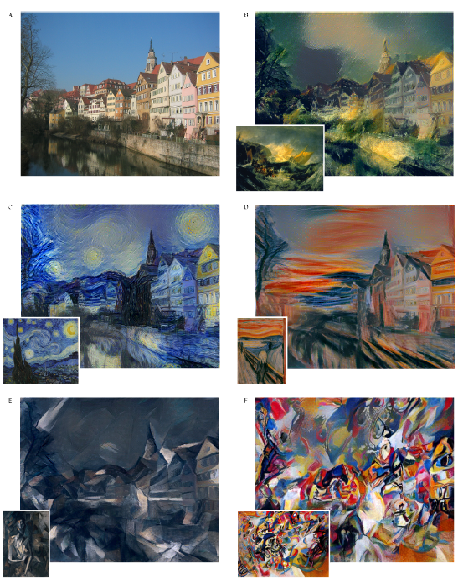
\includegraphics{pics/66.png}
 \caption{Images that combine the content of a photograph with the style of several well-known artworks.}
 \label{fig:6.6}
\end{figure}
说到这里,对卷积神经网络比较熟悉的可以想到,中层的卷积特征符合这两个特性。在我们还未明确什么是风格这个特征的时候,可以找一个比较大的网络(例如vgg),将中层卷积特征的分布当做风格。

这篇文章主要解决了两个问题:
\begin{enumerate}
  \item 如何能同时保证生成的图像还像原来的东西,即”这个东西原来是什么,现在还是什么“。语义(semantic),处在神经网络的高层中。因此原图和结果图的高层语义特征之差应尽量小。
  \item “风格”这个pattern到底是什么,文中的答案是所有卷积层的特征,这跟我们上边分析得到的“中层特征”不是很相符,高层特征会带来一些具体的物体,比如梵高星空中的大漩涡,窃以为这个具体的物体不叫风格。
\end{enumerate}

为了实现平移不变性,作者使用了所有空间位置上,特征的协方差矩阵来衡量特征的分布。通过减小原图和风格图的特征分布之间的差距,使得原图和风格图的风格尽量接近。

上边提到了两个”减小“,对应着两个损失函数,通过优化,即可得到文中所示的结果。

这篇工作是开创性的,即找到了新的应用,所以很值得肯定。但是并不能称作为革命性的成果。文章中的style reconstruction的loss 的定义上面,这个作者并没有阐述他们的intuition,但是可以预见的是这个参数应该是纯粹经验性的。


\section{进一步的阅读和总结}
%---------------------------------------------
\chapterimage{chapter_head_8.jpg}
\chapter{递归神经网络RNN}
前馈神经网络的输入和输出的维数都是固定的,不能任意改变。当处理序列数据时,前馈神经网络就无能力为了。因为序列数据是变长的。为了使得前馈神经网络能处理变长的序列数据,一种方法是使用延时神经网络(Time-Delay Neural Networks,TDNN)\cite{waibel1989phoneme}。

\textbf{循环神经网络}(Recurrent Neural Network,RNN),也叫\textbf{递归神经网络}。这里为了区别与另外一种\textbf{递归神经网络}(Recursive Neural Network),我们称为循环神经网络。在前馈神经网络模型中,连接存在层与层之间,每层的节点之间是无连接的。

循环神经网络通过使用带自反馈的神经元,能够处理任意长度的序列。循环神经网络比前馈神经网络更加符合生物神经网络的结构。循环神经网络已经被广泛应用在语音识别、语言模型以及自然语言生成等任务上。

给定一个输入序列$\boldsymbol{x}^{(1:n)}= (\boldsymbol{x}^{(1)},\boldsymbol{x}^{(2)},...,\boldsymbol{x}^{(t)},\cdots ,\boldsymbol{x}^{(n)})$,循环神经网络通过下面公式更新带反馈边的隐藏层的\textbf{活性值}$\boldsymbol{h}(t)$:
\begin{equation}\label{7.1}
  \boldsymbol{h}_t =
  \begin{cases}
   0 & \text{if } t= 0 \\
   f(\boldsymbol{h}_{t-1},\boldsymbol{x}_t)       & \text{if } otherwise
  \end{cases}
\end{equation}
从数学上讲,式\ref{7.1}可以看成一个\textbf{动态系统}。动态系统是指系统的状态按照一定的规律随时间变化的系统。因此,活性值$\boldsymbol{h}_t$在很多文献上也称为\textbf{状态}。但这里的状态是数学上的概念,区别与我们在前馈网络中定义的神经元的状态。理论上循环神经网络可以近似任意的动态系统。图\ref{fig:7.1}给出了循环神经网络的示例。
\begin{figure}[t]
 \centering
 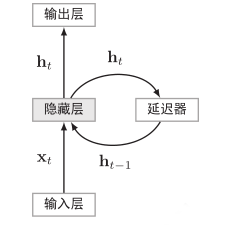
\includegraphics{pics/71.png}
 \caption{RNN}
 \label{fig:7.1}
\end{figure}
循环神经网络的参数训练可以通过随时间进行反向传播(Backpropagation Through Time,BPTT)算法\cite{werbos1990backpropagation}。但循环神经网络的一个最大问题是训练时梯度需要随着时间进行反向传播。当输入序列比较长时,会存在梯度爆炸和消失问题\cite{bengio1994learning,hochreiter1997long,hochreiter2001gradient}。 长短时记忆神经网络(long short term memory neural network,LSTM)\cite{hochreiter1997long}是训练神经网络的一个扩展。
\section{简单的递归网络}
我们先来看一个非常简单的循环神经网络,叫\textbf{简单循环网络}(Simple Recurrent Network,SRN)\cite{elman1990finding}。

假设时刻$t$时,输入为$\boldsymbol{x}_t$,隐层状态(隐层神经元活性)为$\boldsymbol{h}_t$。$\boldsymbol{h}_t$ 不仅和当前时刻的输入相关,也和上一个时刻的隐层状态相关。

一般我们使用如下函数:
\begin{equation}\label{7.2}
  \boldsymbol{h}_t=f(\boldsymbol{U}\boldsymbol{h}_{t-1}+\boldsymbol{W}\boldsymbol{x}_t+\boldsymbol{b})
\end{equation}
这里,$f$是非线性函数,通常为logistic函数或tanh 函数。
\begin{figure}[t]
 \centering
 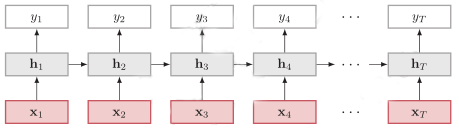
\includegraphics{pics/72.png}
 \caption{Simple RNN expanded by time}
 \label{fig:7.2}
\end{figure}

图\ref{fig:7.2}给出了按时间展开的循环神经网络。
\subsection{梯度}
循环神经网络的参数训练可以通过\textbf{随时间进行反向传播}(Backpropagation Through Time,BPTT)算法\cite{werbos1990backpropagation}。 图\ref{fig:7.3}给出了随时间进行反向传播算法的示例。
\begin{figure}[t]
 \centering
 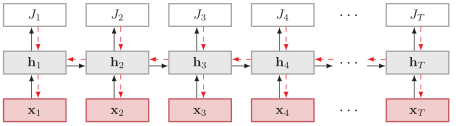
\includegraphics{pics/73.png}
 \caption{RNN expanded by time}
 \label{fig:7.3}
\end{figure}

假设循环神经网络在每个时刻$t$都有一个监督信息,损失为$J_t$。则整个序列的损失为$J=\sum_{t=1}^TJ_t$。

损失$J$关于$U$的梯度为:
\begin{gather}\label{7.3}
  \frac{\partial J}{\partial U} =\sum_{t=1}^T\frac{\partial J_t}{\partial U}\\
  =\sum_{t=1}^T\frac{\partial \boldsymbol{h}_t}{\partial U}\frac{\partial J_t}{\partial \boldsymbol{h}_t}
\end{gather}
其中,$\boldsymbol{h}_t$是关于$U$和$\boldsymbol{h}_{t-1}$的函数,而$\boldsymbol{h}_{t-1}$ 又是关于$U$ 和$\boldsymbol{h}_{t-2}$的函数。因此,我们可以用链式法则得到:
\begin{equation}\label{7.5}
  \frac{\partial J}{\partial U} =\sum_{t=1}^{T}\sum_{k=1}^{t}\frac{\partial \boldsymbol{h}_k}{\partial U}\frac{\partial \boldsymbol{h}_t}{\partial \boldsymbol{h}_k}\frac{\partial \boldsymbol{y}_t}{\partial \boldsymbol{h}_t}\frac{\partial J_t}{\partial \boldsymbol{y}_t}
\end{equation}
其中,
\begin{gather}\label{7.6}
  \frac{\partial \boldsymbol{h}_t}{\partial \boldsymbol{h}_k}=\prod_{i=k+1}^{t}\frac{\partial \boldsymbol{h}_i}{\partial \boldsymbol{h}_{i-1}} \\
  =\prod_{i=k+1}^{t}U^T\boldsymbol{diag}[f'(h_{i-1})]
\end{gather}
因此,
\begin{equation}\label{7.8}
  \frac{\partial J}{\partial U} =\sum_{t=1}^{T}\sum_{k=1}^{t}\frac{\partial \boldsymbol{h}_k}{\partial U}  \left( \prod_{i=k+1}^{t}U^T\boldsymbol{diag}[f'(h_{i-1})] \right)    \frac{\partial \boldsymbol{y}_t}{\partial \boldsymbol{h}_t}\frac{\partial J_t}{\partial \boldsymbol{y}_t}
\end{equation}

我们定义$\gamma = ||U^T\boldsymbol{diag}[f'(h_{i-1})]||$,则在上面公式中的括号里面为$\gamma^{t-k}$。 如果$\gamma > 1$,当$t-k \to \inf$ 时,$\gamma^{t-k}\to \infty$,会造成系统不稳定,也就是所谓的梯度爆炸问题;相反,如果$\gamma < 1$,当$t-k \to \infty$ 时,$\gamma^{t-k}\to 0$,会出现和深度前馈神经网络类似的梯度消失问题。

在训练循环神经网络时,更经常出现的是梯度消失问题。因为我们一般情况下使用的非线性激活函数为logistic函数或tanh 函数,其导数值都小于$1$。 而权重矩阵$∥U^T∥$也不会太大。我们定义$||U^T|| \leq \gamma_u\leq 1$,$||\boldsymbol{diag}[f'(h_{i-1})]|| \leq \gamma_f\leq 1$,则有:
\begin{equation}\label{7.9}
  ||\frac{\partial \boldsymbol{h}_i}{\partial \boldsymbol{h}_{i-1}}||\leq ||U^T|| \cdot ||\boldsymbol{diag}[f'(h_{i-1})]|| \leq \gamma_u\gamma_f\leq 1
\end{equation}
经过$t - k$次传播之后,
\begin{equation}\label{7.10}
  ||\frac{\partial \boldsymbol{h}_i}{\partial \boldsymbol{h}_{i-1}}||\leq(\gamma_u\gamma_f)^{t-k}
\end{equation}
如果时间间隔$t - k$过大,$||\frac{\partial \boldsymbol{h}_i}{\partial \boldsymbol{h}_{i-1}}||$会趋向于0。

因此,虽然简单循环网络从理论上可以建立长时间间隔的状态之间的依赖关系(Long-Term Dependencies),但是由于梯度爆炸或消失问题,实际上只能学习到短周期的依赖关系。这就是所谓的\textbf{长期依赖问题}。
\subsection{改进方案}
为了避免梯度爆炸或消失问题,关键是使得$U^T\boldsymbol{diag}[f'(h_{i-1})] = 1$。 一种方式就是选取合适的参数,同时使用非饱和的激活函数。但这样的方式需要很多人工经验,同时限制了模型的广泛应用。

还有一种方式就是改变模型,比如让$U = 1$,同时使用$f′(\boldsymbol{h}_{i-1}) = 1$。
\begin{equation}\label{7.11}
  \boldsymbol{h}_t=\boldsymbol{h}_{i-1}+\boldsymbol{W}\boldsymbol{g}(\boldsymbol{x}_t)
\end{equation}
$\boldsymbol{g}$是非线性激活函数。

但这样的形式,丢失了神经元在反馈边上的非线性激活的性质。因此,一个更加有效的改进是引入一个新的状态$\boldsymbol{c}_t$专门来进行线性的反馈传递,同时在$\boldsymbol{c}_t$的信息非线性传递给$\boldsymbol{h}_t$。
\begin{gather}\label{7.12}
  \boldsymbol{c}_t=\boldsymbol{c}_{t-1}+\boldsymbol{W}\boldsymbol{g}(\boldsymbol{x}_t) \\
  \boldsymbol{h}_t=\tanh{\boldsymbol{c}_t}
\end{gather}

但是,这样依然存在一定的问题。因为$\boldsymbol{c}_t$和$\boldsymbol{c}_{t-1}$ 是线性关系,同时不断累积$\boldsymbol{x}_t$ 的信息,会使得$\boldsymbol{c}_t$变得越来越大。为了解决这个问题,Hochreiter and Schmidhuber\cite{hochreiter1997long} 提出一个非常好的解决方案,就是引入门机制(Gating Mechanism)来控制信息的累积速度,并可以选择遗忘之前累积的信息。这就是下面要介绍的\textbf{长短时记忆神经网络}。
\section{长短时记忆神经网络:LSTM}

\textbf{长短时记忆神经网络}(Long Short-Term Memory Neural Network,LSTM)\cite{hochreiter1997long}是循环神经网络的一个变体,可以有效地解决简单循环神经网络的梯度爆炸或消失问题。

LSTM模型的关键是引入了一组记忆单元(Memory Units),允许网络可以学习何时遗忘历史信息,何时用新信息更新记忆单元。在时刻t 时,记忆单元$\boldsymbol{c}_t$记录了到当前时刻为止的所有历史信息,并受三个“门”控制:输入门$\boldsymbol{i}_t$, 遗忘门$\boldsymbol{f}_t$和输出门$\boldsymbol{o}_t$. 三个门的元素的值在$[0,1]$ 之间。

在时刻$t$时LSTM的更新方式如下:

\begin{gather}\label{7.14}
  \boldsymbol{i}_t=\sigma(W_i\boldsymbol{x}_t+U_i\boldsymbol{h}_{t-1}+V_i\boldsymbol{c}_{t-1}) \\
  \boldsymbol{f}_t=\sigma(W_f\boldsymbol{x}_t+U_f\boldsymbol{h}_{t-1}+V_f\boldsymbol{c}_{t-1})\\
  \boldsymbol{o}_t=\sigma(W_o\boldsymbol{x}_t+U_o\boldsymbol{h}_{t-1}+V_o\boldsymbol{c}_{t-1})\\
  \widetilde{\boldsymbol{c}_t}=\tanh(W_c\boldsymbol{x}_t+U_c\boldsymbol{h}_{t-1})\\
  \boldsymbol{c}_t=\boldsymbol{f}_t\odot \boldsymbol{c}_{t-1}+\boldsymbol{i}_t\odot \widetilde{\boldsymbol{c}_t}\\
  \boldsymbol{h}_t=\boldsymbol{o}_t\odot\tanh{\boldsymbol{c}_t}
\end{gather}
这里,$\boldsymbol{x}_t$是当前时刻的输入,$\sigma$是logistic函数,$V_i$,$V_f$,$V_o$是对角矩阵。遗忘门$\boldsymbol{f}_t$控制每一个内存单元需要遗忘多少信息,输入门$\boldsymbol{i}_t$ 控制每一个内存单元加入多少新的信息,输出门$\boldsymbol{o}_t$控制每一个内存单元输出多少信息。
\begin{figure}[t]
 \centering
 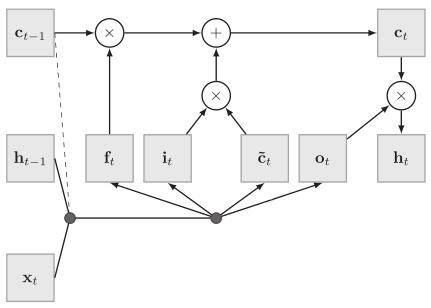
\includegraphics{pics/74.png}
 \caption{LSTM Structure Expamle}
 \label{fig:7.4}
\end{figure}

图7.4给出了LSTM模型的计算结构。

这样,LSTM可以学习到长周期的历史信息。

LSTM已经被应用到很多的任务中,比如机器翻译\cite{sutskever2014sequence} 等。
\section{门限循环单元:GRU}
门限循环单元(Gated Recurrent Unit,GRU)\cite{cho2014learning,chung2014empirical}是一种比LSTM更加简化的版本。在LSTM 中,输入门和遗忘门是互补关系,因为同时用两个门比较冗余。GRU 将输入门与和遗忘门合并成一个门:更新门(Update Gate),同时还合并了记忆单元和神经元活性。

GRU模型中有两个门:更新门$\boldsymbol{z}$ 和重置门$\boldsymbol{r}$。 更新门$\boldsymbol{z}$ 用来控制当前的状态需要遗忘多少历史信息和接受多少新信息。重置门$\boldsymbol{r}$用来控制候选状态中有多少信息是从历史信息中得到。

GRU模型的更新方式如下:
\begin{gather}\label{7.20}
  \boldsymbol{r}_t=\sigma(\boldsymbol{W}_r)\boldsymbol{x}_t+\boldsymbol{U}_r \boldsymbol{h}_{t-1} \\
  \boldsymbol{z}_t=\sigma(\boldsymbol{W}_z)\boldsymbol{x}_t+\boldsymbol{U}_z \boldsymbol{h}_{t-1}\\
  \widetilde{\boldsymbol{h}_t}=\tanh(\boldsymbol{W}_c\boldsymbol{x}_t+\boldsymbol{U}(\boldsymbol{r}_z\odot\boldsymbol{h}_{t-1}))\\
  \boldsymbol{h}_t=\boldsymbol{z}_t\odot\boldsymbol{h}_{t-1}+(1-\boldsymbol{z}_t)\odot\widetilde{\boldsymbol{h}_t}
\end{gather}

这里选择$\tanh$函数也是因为其导数有更大的值域。
\section{一个强大的RNN框架:DeepNet}
\section{一些经典论文基于DeepNet的实验重现}
\section{进一步的阅读和总结}

%----------------------------------------------------------------------------------------
%	BIBLIOGRAPHY
%----------------------------------------------------------------------------------------
\chapterimage{bibliography_head.jpg}
\chapter*{Bibliography}

\addcontentsline{toc}{chapter}{\textcolor{ocre}{Bibliography}}
%\begin{thebibliography}{}
%\bibliographystyle{plain}
%\bibliography{bibliography}
%\end{thebibliography}
%------------------------------------------------

%$\section*{Articles}
%\addcontentsline{toc}{section}{Articles}

\printbibliography[heading=bibempty]
%\printbibliography[heading=bibempty,type=InProceedings],type=article
%\printbibliography[heading=bibempty,type=Unpublished]
%\printbibliography[heading=bibempty,type=Misc]

%------------------------------------------------

%\section*{Books}
%\addcontentsline{toc}{section}{Books}
%\printbibliography[heading=bibempty,type=book]


%----------------------------------------------------------------------------------------
%	INDEX
%----------------------------------------------------------------------------------------

%\cleardoublepage
%\phantomsection
%\setlength{\columnsep}{0.75cm}
%\addcontentsline{toc}{chapter}{\textcolor{ocre}{Index}}
%\printindex
%----------------------------------------------------------------------------------------
%	APPENDX
%----------------------------------------------------------------------------------------


%\appendixpage
%\addcontentsline{toc}{chapter}{Appendices}\markboth{APPENDICES}{附录}
\begin{subappendices}
\part{附录 APPENDICES}
%---------------------------------------------
\chapterimage{appendex_head.jpg}
\chapter{学习理论的统计机理}
这一部分(Statistical Mechanics of Learning)我们将介绍一些统计学上的原理和方法,以及这方法在神经网络中的量化研究。\textbf{该附录的理解需要相当部分的数学知识,选择阅读}。

\section{一些约定}
数学上的分析可能只能对一些极端的结构奏效。这里我们关心两种神经网络:第一种极端情况是全互联如图\ref{fig:app1}.b,其动态结构是高复发的,并且其结果将是神经元不同活动模式的混沌序列;另一种极端情况称为前馈神经网络(feed-forward neural network, FFN)如图\ref{fig:app1}.c,其神经元可以被排序为layers $l=1,\cdots,L$,使得在$l$ 层的每个神经元仅会收到来自$l-1$层神经元的input并仅会前馈给$l+1$层的神经元。第一层$l=1$称输入层,最后一层$l=L$称输出层,其余$1<l<L$称隐层。

由于缺失反馈回路,其动态性能将会相当简单:输入将通过连续过程映射到输出层。因此,会表现出从输入到输出标签的分类性,通过输出层的不同配置。这个结构是非常适合作为学习之用,最特殊的就是感知器。

\begin{figure}[t]
 \centering
 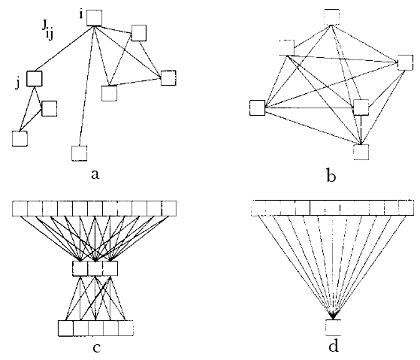
\includegraphics{pics/app1.png}
 \caption{不同类型的神经网络:a)普适结构,b)全链接吸引神经网络,c)带一个隐层的反馈神经网络,d) 单层感知器}
 \label{fig:app1}
\end{figure}
\subsection{Annealed Analysis of Gibbs Learning}
对输入$\boldsymbol{S}$到感知器$\boldsymbol{J}$的classification $sgn(\boldsymbol{JS})$,这里给出一个几何上的解释:
\begin{equation*}
  sgn(\boldsymbol{JS}) =
  \begin{cases}
    1       & \langle\boldsymbol{J},\boldsymbol{S}\rangle>\pi/2\\
    -1  & \langle\boldsymbol{J},\boldsymbol{S}\rangle<\pi/2\\
  \end{cases}
\end{equation*}
这里,$1,-1$被称为\textbf{决策边界},可以理解为自输入的半平面分类;也是由于这个原因,如果可以通过一个感知器实现的分类被称为\textbf{线性可分}的。

显然,$\boldsymbol{J},\boldsymbol{S}$的length对分类没有影响。为避免不同的耦合(length)的向量被归为相同分类的可能性,对权重和输入均做正则化:
\begin{equation*}
  \boldsymbol{J}^2=\sum_{i=1}^NJ_i^2=N~~~\text{and}~~~\boldsymbol{S}^2=\sum_{i=1}^NS_i^2=N
\end{equation*}
其代表的几何意义为$\boldsymbol{J},\boldsymbol{S}$指向半径为$\sqrt{N}$的$N$维超球面。

为比较二感知器的分类性能:teacher perceptron$\boldsymbol{T}$ and student perceptron $\boldsymbol{J}$,我们讲相同的输入通过二者映射到一个平面上如图\ref{fig:app2}。显而易见的阴影部分是误识区域。如果输入的选择是随机的,那么误识的概率可以精确的表述为generalization error $\varepsilon$。由于分类线是垂直于向量$\boldsymbol{T}~\text{and}~\boldsymbol{J}$的,显然$\varepsilon=\theta/\pi$,这里$\theta$是向量$\boldsymbol{T}~\text{and}~\boldsymbol{J}$的夹角。于是generalization error $\varepsilon$正比于向量在$N$ 维超球面上的几何距离(测地线距)。为方便,我们引入teacher-student overlap:
\begin{equation*}
  R=\frac{\boldsymbol{JT}}{N}
\end{equation*}
然而由于:$\frac{\boldsymbol{JT}}{N}=\frac{\boldsymbol{JT}}{|\boldsymbol{J}|\cdot|\boldsymbol{T}|}=\cos\langle\boldsymbol{J},\boldsymbol{T}\rangle=\cos\theta$,generalization error可以写为:
\begin{equation*}
  \varepsilon=\frac{1}{\pi}\arccos R
\end{equation*}
\begin{figure}[t]
 \centering
 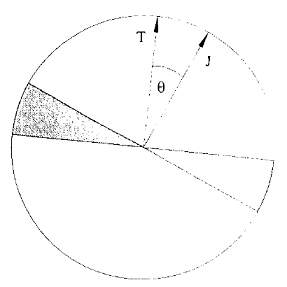
\includegraphics{pics/app2.png}
 \caption{Projection of the input space to the plane spanned by the coupling vectors of teacher and student. Patterns with projection in the shaded region are classified wrongly by student.}
 \label{fig:app2}
\end{figure}

现在我们考虑一个策略以期在学习中修复student的错误。考虑耦合向量$\boldsymbol{J}$ 表征了example完全归为teacher,被\textbf{兼容}的students所组成的几何称为\textbf{version space}。 我们要求generalization error在verison space上随机分布。这个简单的方法(prescription)称为\textbf{Gibbs Learning}。其学习规则的结果被发现可以特征化一个被兼容学生的典型表现(\textbf{the typical performance of a compatible student})。

在Gibbs Learning的框架下,generalization error将会随训练集的规模的上升而下降(由于越来越多的$\boldsymbol{J}$ 被认为不兼容导致的version space的缩小)。如果我们可以量化一个耦合向量的“存活几率”,当一个新example被$\boldsymbol{J}$表征的时候,我们可以得到在训练过程中generalization error的平均表现。显然,根据上面overlap的定义,对每个$\boldsymbol{J}$的存活几率为$1-\arccos R/\pi=1-\varepsilon$。定义$\Omega_0(\varepsilon)$为训练前所有耦合向量$\boldsymbol{J}$的体积,由于每次训练是独立的,那么在第$p$ 次训练后所能兼容student的平均体积为:
\begin{equation*}
  \Omega_p(\varepsilon)=\Omega_0(\varepsilon)(1-\varepsilon)^p
\end{equation*}

显然\footnote{
这里积分的计算使用了$\delta$函数的指数极限式定义:
\begin{equation*}
  \delta(x) = \lim_{a\to 0}\frac{1}{a \sqrt{\pi}} \mathrm{e}^{-x^2/a^2}
\end{equation*}
以下表达式也可代表狄拉克$\delta$函数:
\begin{gather*}
  \delta(x)=\lim_{\alpha\to 0^+}\frac{1}{\pi}\frac{\alpha}{\alpha^2+x^2} \\
  \delta(x)=\frac{1}{2\pi}\int_{-\infty}^{+\infty}e^{ikx}dk \\
  \delta(x)=\lim_{k\to\infty}\frac{1}{\pi}\frac{\sin{kx}}{x}
\end{gather*}
}:
\begin{equation}\label{appa1}
  \Omega_0(\varepsilon)=\int d\boldsymbol{J}\delta(\boldsymbol{J}^2-N)\delta(\frac{\boldsymbol{JT}}{N}-\cos(\pi\varepsilon))\underset{N\to\infty}{\sim} \exp\{\frac{N}{2}[1+\ln2+\ln\sin^2(\pi\varepsilon)]\}
\end{equation}
记:$p=\alpha N$:
\begin{equation}\label{app1}
  \Omega_p(\varepsilon)\underset{N\to\infty}{\sim} \exp\{N[\frac{1}{2}(1+\ln(2\pi))+\frac{1}{2}\ln\sin^2(\pi\varepsilon)+\alpha\ln(1-\varepsilon)]\}
\end{equation}

上式中括号中的表达式已经在图\ref{fig:app3}中画出。注意到这虽然是$\varepsilon$的一个光滑函数,但是相应的$\Omega_p(\varepsilon)$会被指数级因子$\exp N$放大。因此我们可以得出从我们期望的version space通过随机形式选择的student向量的方法。对于较大的$N$,可以以压倒性的概率选择一个使图\ref{fig:app3}中函数最大的$\varepsilon$。 所有其他的$\varepsilon$值可以认为对应的指数级稀少的耦合向量。我们因此希望在较大的$N$极限下,generalization error可以由下式表示:
\begin{equation*}
  \varepsilon(\alpha)=\argmax[\frac{1}{2}\ln\sin^2(\pi\varepsilon)+\alpha\ln(1-\varepsilon)]
\end{equation*}
对于$\alpha=0$,$\Omega_p(\varepsilon)$在$\varepsilon=5$时取得最大值,对应student与teacher正交。显然,没有更进一步的信息,所有$\boldsymbol{J}$的选择是平权的,并且那些随机表现的students在数量上指数级的压倒了其他的。在学习过程中,这个效果会被来自训练集所包含的信息自动抵消,在Gibbs Learing中也即是\ref{app1} 中$\alpha\ln(1-\varepsilon)$。对于一个大的训练集,generalization error会越来越小,当$\alpha\to0$时,$\varepsilon\to\infty$
\begin{figure}[t]
 \centering
 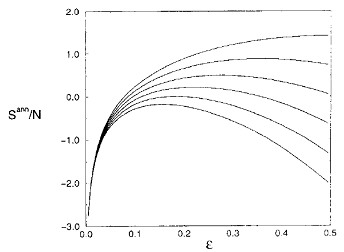
\includegraphics{pics/app3.png}
 \caption{Expression of \ref{app1} as a function of $\varepsilon$ for $\alpha=0,1,2,3,4\text{ and }5$ (from top to bottom)}
 \label{fig:app3}
\end{figure}

以上的结果也提供了关于ANN如何从example中学习的量化指标。首先,网络的特殊结构蕴含了一种可实现的先验层级映射,“简单的”输入输出关系可以被相当多不同的耦合向量实现,而“困难的”则需要微观层面的细节配置。这种层级关系可以被称为系统的偏见。其次,训练集中无可比拟的分类被清除,这种形式的学习本质蕴含了精准性和灵活性的取舍。一个拥有能实现所有映射的系统,原则上能学习任何问题,但是过于广泛的特征也会导致对每个具体问题的处理相同的弱;另一方面,一个非常特殊的系统可能只能对某个限制的问题学习,但是可以比其他的模型做的更好。事实上,类似惊人的"Eureca!"突然转变到完美的普适形式会在这种系统中出现。

为了了解我们为Gibbs Learning的简单分析的正确性,我们将\ref{app1}的结论以点线图在图\ref{fig:app4}中绘出。在与仿真的对比中,我们清晰的发现虽然数值表现的大势所趋被正确表述,并且对于足够大的$\alpha$,我们有:
\begin{equation*}
  \varepsilon\sim\frac{1}{\alpha}
\end{equation*}
但是根据错误前因子给出的正确缩放尺度下在数值上的拟合是很弱的。

\begin{figure}[t]
 \centering
 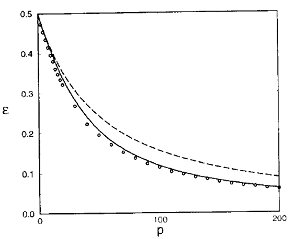
\includegraphics{pics/app4.png}
 \caption{Simulation results(circles) for the generalization error of a perceptron learning from example to rank dual numbers. The results are averaged over 1000 realizations of the training set, the statistical error is smaller than the symbol size. The full line gives the analytic results if the quenched calculation, the dashed line that of the annealed approximation.}
 \label{fig:app4}
\end{figure}

所以我们的分析错在哪里?主要的错误是我们没有正确处理学习样本$\boldsymbol{\xi}^{\mu}$和teacher耦合向量$\boldsymbol{T}$的随机性。我们用$\Omega(\varepsilon:\boldsymbol{\xi}^{\mu},\boldsymbol{T})$来表示经过$p$ 个样本$\boldsymbol{\xi}^{\mu}$学习后的student耦合向量与teacher耦合向量$\pi\varepsilon$夹角范围内剩余version space的大小。由于$\boldsymbol{\xi}^{\mu}$和$\boldsymbol{T}$均是随机选取的,所以$\Omega(\varepsilon:\boldsymbol{\xi}^{\mu},\boldsymbol{T})$的取值也应该是随机的。然而,上面定义的$\Omega_p(\varepsilon)$是以平均意义下描述的。在很多情况下,平均描述可以有意义地给出给出随机系统的典型描述。但是这不是总是成立的,尤其是对于$\Omega(\varepsilon:\boldsymbol{\xi}^{\mu},\boldsymbol{T})$。作为结果,对于压倒性概率足够大的$N$,$\Omega(\varepsilon:\boldsymbol{\xi}^{\mu},\boldsymbol{T})$的取值是不同于\ref{appa1} 中的平均描述。事实上,我们可以说明\ref{app1}总是给出了$\varepsilon$ 的上界。

为了表示在足够大$N$情况下不能被很好平均表述的$\Omega(\varepsilon:\boldsymbol{\xi}^{\mu},\boldsymbol{T})$的分布,更重要的是找到一个正确的方式来描述$\varepsilon(\alpha)$的典型表现。使用统计机理框架下的逼近是很有用的。为表达这些框架,我们会建立针对学习问题量化分析的中心统计机理技巧(Central Statistical Mechanics Techniques for the Quantitative Analysis of Learning Problems)。
\subsection{The Annealed Approximation in Statistical Mechanics}
我们来重述一下在统计观点下的学习机制。微观变量$J_i$组成student向量,其span\footnote{
Given a vector space $V$ over a field $K$, the span of a set $S$ of vectors (not necessarily finite) is defined to be the intersection $W$ of all subspaces of $V$ that contain $S$. $W$ is referred to as the subspace spanned by $S$, or by the vectors in $S$. Conversely, $S$ is called a spanning set of $W$, and we say that $S$ spans $W$.

Alternatively, the span of $S$ may be defined as the set of all finite linear combinations of elements of $S$, which follows from the above definition.
\begin{equation*}
  \operatorname{span}(S) =  \left \{ {\sum_{i=1}^k \lambda_i v_i \Big| k \in \mathbb{N}, v_i  \in S, \lambda _i  \in \mathbf{K}} \right \}.
\end{equation*}

In particular, if $S$ is a finite subset of $V$, then the span of $S$ is the set of all linear combinations of the elements of $S$. In the case of infinite $S$, infinite linear combinations (i.e. where a combination may involve an infinite sum, assuming such sums are defined somehow, e.g. if $V$ is a Banach space) are excluded by the definition; a generalization that allows these is not equivalent.
}(线性张成空间)组成相空间。generalization error $\varepsilon$也是微观相关的。给定值的$\varepsilon$可能被不同微观选择的$\boldsymbol{J}$实现。在统计学中,一个重要的量化指标:熵$S$:
\begin{equation}\label{appa11}
  S(\varepsilon:\boldsymbol{\xi}^{\mu},\boldsymbol{T})=\ln\Omega(\varepsilon:\boldsymbol{\xi}^{\mu},\boldsymbol{T})
\end{equation}
显然,在学习之前对于足够大$N$:
\begin{equation}\label{appa12}
  S_0(\varepsilon)\sim\frac{N}{2}[1+\ln2\pi\ln\sin^2(\pi\varepsilon)]
\end{equation}
熵表现出其广阔特性,即是$N$为系统的自由度。

式\ref{appa12}的前两项是独立于$\varepsilon$的,并且对应$N$维超球面。这对$\Omega(\varepsilon:\boldsymbol{\xi}^{\mu},\boldsymbol{T})$的正则化是相当方便的,为此,我们定义积分测度:
\begin{equation}\label{appa13}
  d\mu(\boldsymbol{J})\equiv\frac{d\boldsymbol{J}\delta(\boldsymbol{J}^2-N)}{\int d\boldsymbol{J}\delta(\boldsymbol{J}^2-N)}
\end{equation}
以保证$\int d\mu(\boldsymbol{J})=1$。重整化后的熵可以简写为:
\begin{equation}\label{appa14}
  S_0(\varepsilon)\sim\frac{N}{2}[\ln\sin^2(\pi\varepsilon)]
\end{equation}

在学习的过程中,由于训练样本$\boldsymbol{\xi}^{\mu}$的完善,越来越多的$\boldsymbol{J}$被抛出。函数:
\begin{equation}\label{appa15}
  \chi(\boldsymbol{J})=\prod_{\mu=1}^p\theta((\frac{1}{\sqrt{N}}\boldsymbol{T}\boldsymbol{\xi}^{\mu})(\frac{1}{\sqrt{N}}\boldsymbol{J}\boldsymbol{\xi}^{\mu}))
\end{equation}
取1当所有$\boldsymbol{J}$均被样本分类正确;否则取0。它将作为剩余version space的指标函数。


\section{The Gardner Analysis}
\section{Learning by Minimizing Cost Functions}
\section{Noisy Teachers}
\section{Variations of Preceptron Learning}
\end{subappendices}
%----------------------------------------------------------------------------------------

\end{document}
